As described in Section~\ref{sec:2}, the heavy resonance predicted by many BSM play a key role in understanding many fundamental phenomena. The narrow heavy resonance which decays into two gluons final state at the LHC, appears to be two hadronic jets in the detector. Produced by the QCD processes, the dijet events have a smoothly falling distribution of the invariant mass \mjj, whereas two jets appear to be a resonance in the \mjj spectrum. As a result, searches for dijet resonance are one of the flagship exotics analyses in ATLAS.


Besides, on the assumption that the resonant sample can be classified according to the type of parton that initiated the jets, the sensitivity of searches for new resonance can be improved by identifying the types of partons through which the potentially new particle interact.  One of simplest examples of such tagging is gluon-tagging one or more of the jets. The jet tagging procedure based on the number of
charged tracks with transverse momentum \pt~above 500 GeV is described in Section.~\ref{sec:5}. The \mjj spectrum of background is estimated from the data, which is used for the search in three categories: inclusive, single-gluon, and double-gluon tagged dijet systems. The inclusive \mjj spectrum is thus considered as control region for quark/gluon studies.



This chapter describes searches for new heavy particles decay in dijet final state as originating from gluons or quarks, a technique of quark/gluon tagging is employed to enhance the sensitivity to the results. The search performed uses full Run 2 data at $\sqrt{s} = 13$ TeV, with higher integrated luminosity compared to previous one (Run 1), significantly improvements in the understanding of systematic uncertainties are expected. On the other hand,  cross section upper limits will be set if no significantly resonances are observed.

The simplified procedures in this analysis is performed as following: 
\begin{itemize}
	\item Search for high-mass resonances in the untagged (inclusive), single-gluon tagged,
	and two-gluon tagged categories with dijet events.
	\item If significant resonances are found, claim something interesting, else the upper limits are set. 
	\item Model independent upper-limits are set on resonance cross sections in
	inclusive, single-gluon tagged, and two-gluon tagged categories.
	\item For the specific resonance model, set lower limits on the relevant scales in inclusive, single-gluon tagged, and two-gluon tagged categories.
\end{itemize}

\subsection{Monte Carlo models}
\label{sec:benchmark_signals}.  % uncomment if label used. 
This section outlines benchmark models for both background from the QCD and for new
physics signals that encapsulated in the models chosen:
\Hprime\ , Strings, and QBH.
Full Run 2 data are used to produce EXOT2 skimmed samples used in this analysis.

\subsubsection{QCD background}
\label{qcdsamps}

QCD processes from the MC are simulated at LO and NLO in SM perturbative theory. Due to the large range in cross section of QCD sample, the samples are thus sliced based on the leading jet \pt,  to obtain comparable statistical precision across the jet \pt~range of interest.

% reweighting the underlying spectrum is described in Ref.~\cite{Marshall:2016630}.  


\subsubsection{\Hprime}
\label{sec:hprime}

This analysis performs a model-independent search for two-gluon resonances at high \mjj spectrum, as the CCD background is dominated by valence quark scattering, gluon tagging in this case could be effective. 

The simulated SU(3) singlet scalar that decay via \pythia8 with the A14 set of tuned 
parameters is used in this analysis\footnote{See \url{https://its.cern.ch/jira/browse/ATLMCPROD-6155}.}. The HiggsBSM:gg2H2, where set the singlet scalar as H2 particle and has Particle Data Group ID 35. Such H2 particle is set to decay to gluons and has a narrow resonances width of 0.1 GeV as the physical width is 
model-dependent but constrained by the detector resolution.

The benchmark signals used vary in their underlying physics motivation, but also in the resulting shape of the signal \mjj distribution. The peaks of signal shape are set for various mass points as shown in Figure~\ref{fig:shape_Hprime}, the distributions are normalized to unity and thus the differences in peak amplitudes are not the changes in cross section.

\begin{figure}[htb]
\centering
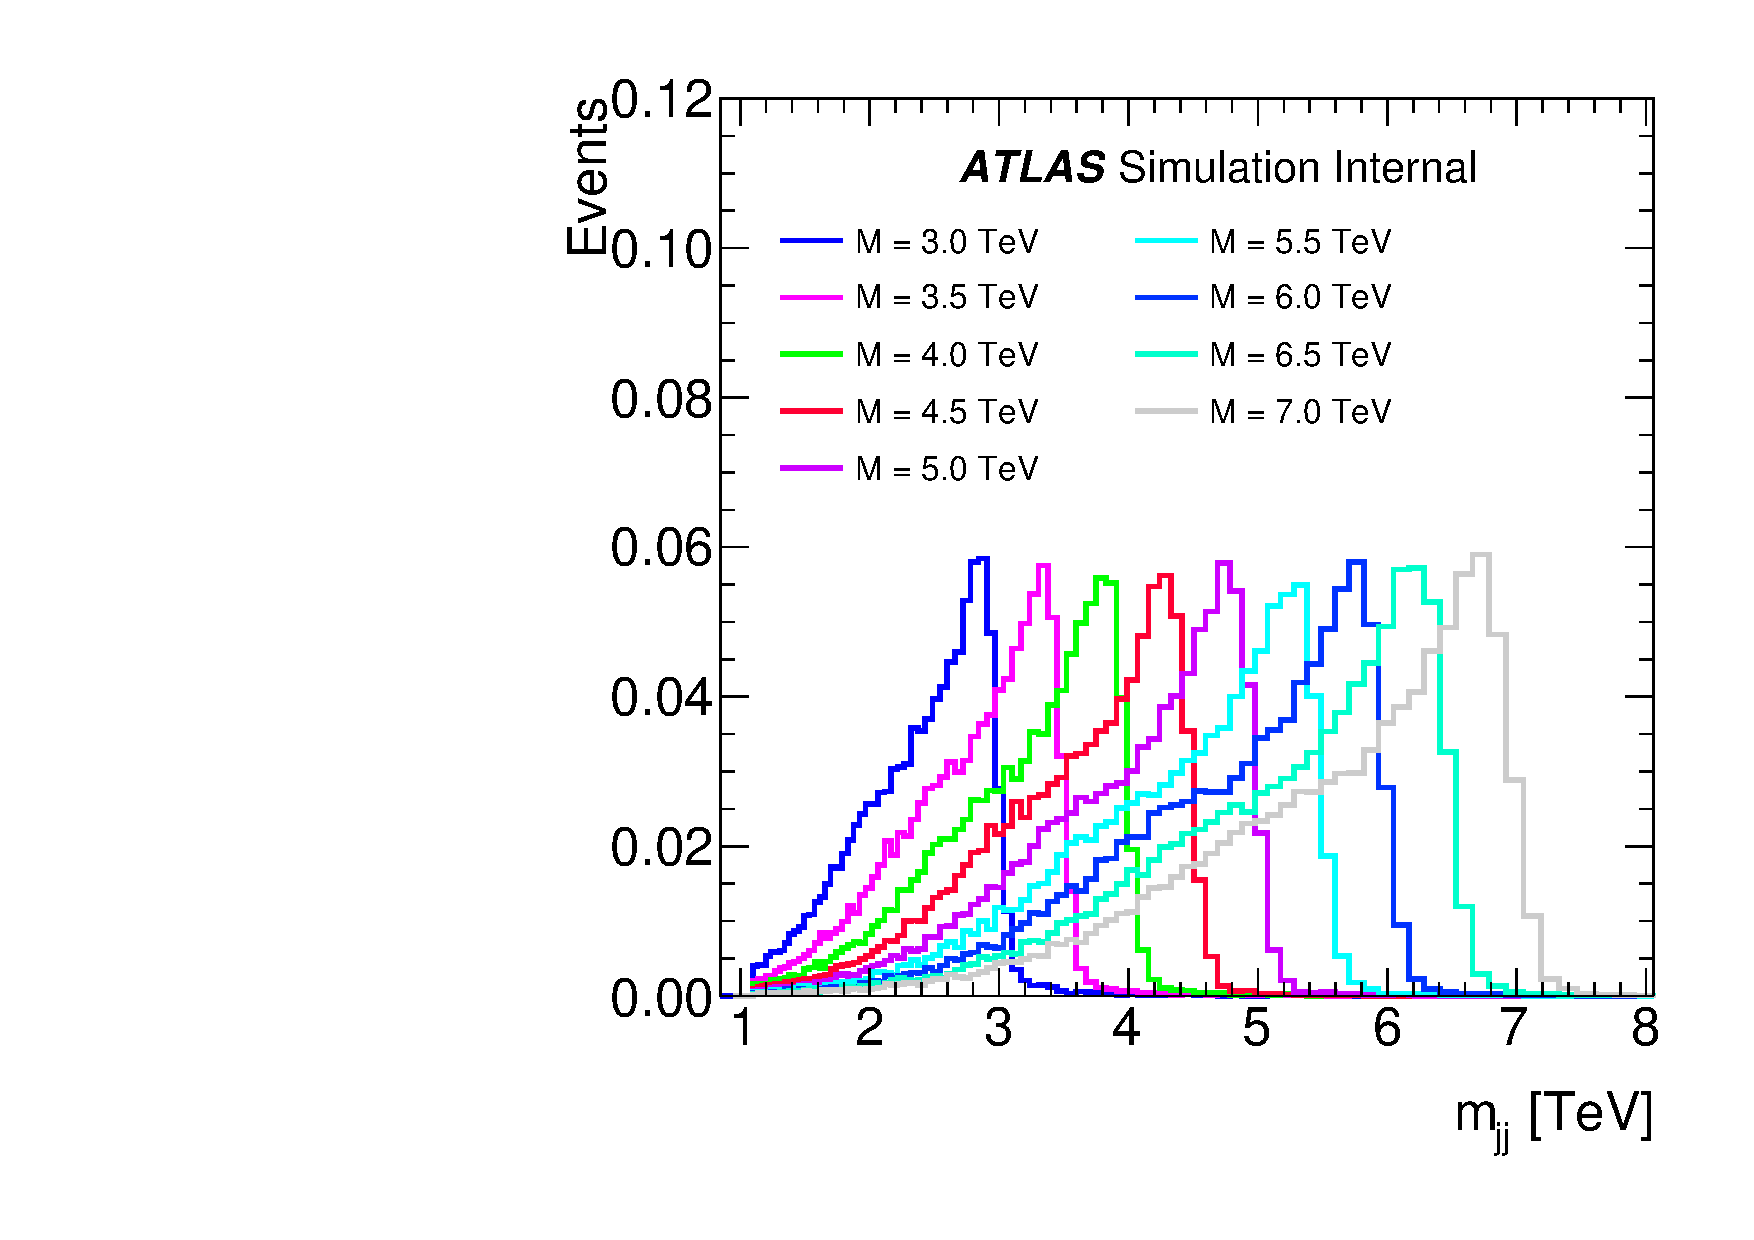
\includegraphics[width=0.48\textwidth]{fig/benchmark_signals/SignalShape-Hprime.pdf}
\caption{Signal shapes for the \Hprime signal at different mass points.}
\label{fig:shape_Hprime}
\end{figure}
\FloatBarrier

\subsubsection{Strings}
\label{sec:string} % uncomment if label used. 
As the SM has lots of well known problems such as the quadratically divergent corrections to the Higgs self-energy, supersymmetry theory offers a solution to it by fine-tuning the
cancellation. The superstring theory, additioal to the supersymmetry, can perform as a framework that unify theories from SM at TeV-scale to quantum gravity at Planck-scale . 

The fundamental string scale is chosen to be within TeV scale, dontes as string mass-scale \Ms~. The string resonances could happen at masses $m_n = \sqrt{n} \Ms$, for $n = 1, 2, 3, \ldots$, where the resonance consist of the Regge excitations of quark, gluon, as well as the colour singlet that lives on the QCD stack of branes. In total, five string scales \Ms range from 7.0~TeV to 9.0~TeV, in steps of 0.5~TeV are generated for string-resonance samples. The lower limits of mass $M_\mathrm{min}$ provided in the generator are shown in Table~\ref{tab1}, together with the resulting cross section of the string samples.

%The string-resonance widths have been calculated in Ref~\cite{Anchordoqui:2008hi}. 

\begin{table}[htb]
\begin{center}
\begin{tabular}{ccc}
\toprule
%[-2ex]
\Ms & $M_\mathrm{min}$ & Cross section\\
{[TeV]} & {[TeV]} & {[fb]}\\ 
\midrule 
\num{7.0} & \num{6.06} & \num{7.09E+0}\\
\num{7.5} & \num{6.60} & \num{1.86E+0}\\
\num{8.0} & \num{7.14} & \num{4.56E-1}\\
\num{8.5} & \num{7.60} & \num{1.00E-1}\\
\num{9.0} & \num{8.05} & \num{1.99E-2}\\
\bottomrule
\end{tabular}
\end{center}
\caption{MC string-resonance samples with string scale \Ms,
minimum mass $M_\mathrm{min}$, and cross section.} 
\label{tab1}
\end{table}

As the string resonances have long Breit-Wigner tails, the PDFs at low-$x$ (low mass) can significantly enhance the tail. In this study, the low-mass tail is truncated since only narrow-resonance structure in \mjj spectrum is interesting to this analysis. In the range $7.0 \leq \Ms \leq 8.0$~TeV, the truncation is done at the minimum value in the differential cross section on the lower-mass side of the \Ms peak, results in around 95\% of the area under the Breit-Wigner curve. In the range $7.0 \leq \Ms \leq 8.0$~TeV, the truncation is done at at a lower-mass point that covers 95\% of the area under the Breit-Wigner curve.

The distribution of signal peak at different mass points is shown in Figure~\ref{fig:shape_strings}, the distributions are normalized to unity and thus the differences in peak amplitudes are not the changes in cross section.

\begin{figure}[htb]
\centering
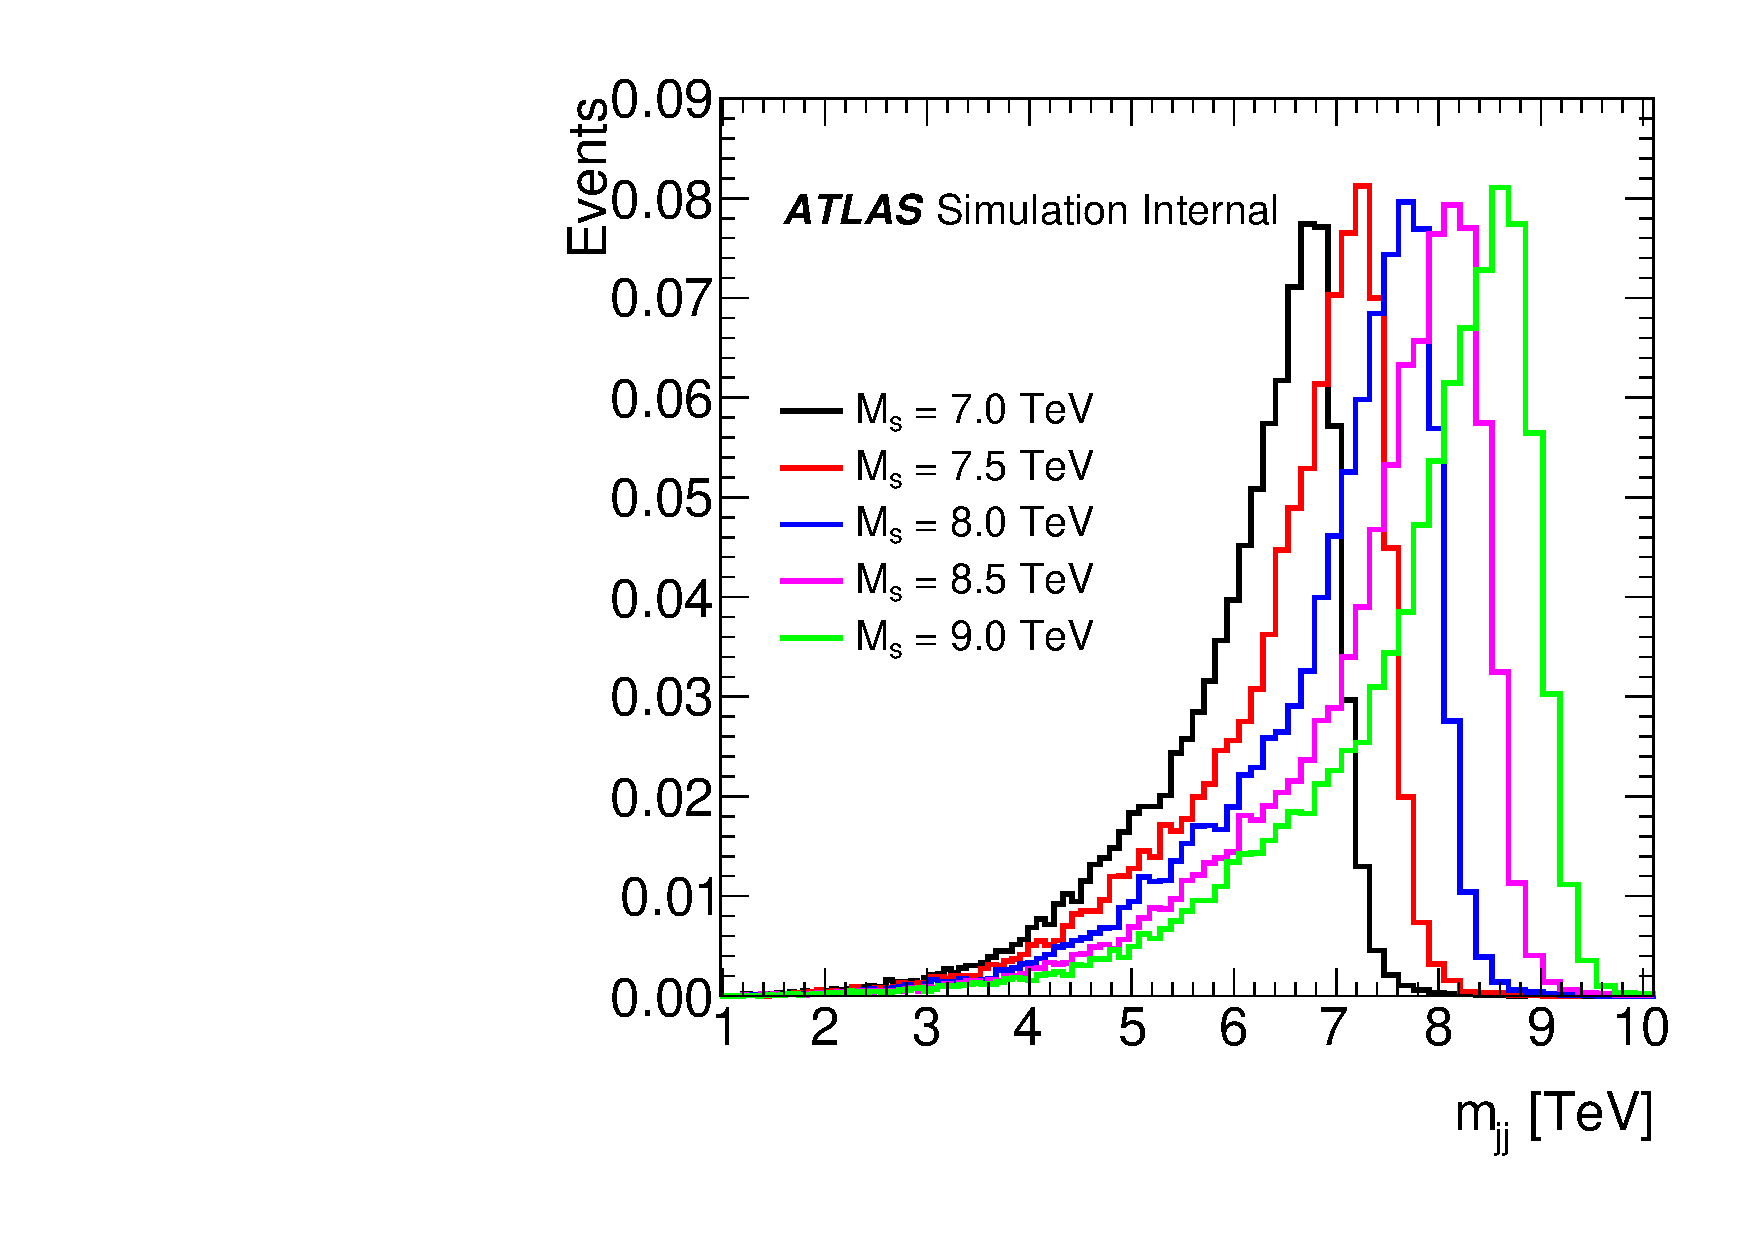
\includegraphics[width=0.48\textwidth]{fig/benchmark_signals/SignalShape-strings.pdf}
\caption{Signal shapes for the String signal.}
\label{fig:shape_strings}
\end{figure}


There are five possible $2\to 2$ subprocesses from string resonances are simulated. with the cross section for each subprocess vary as a function of \Ms shown in Table~\ref{tab2}. The dominate subprocess across the \Ms values is considered to be $gq\to gq$, which contributes around 81-87\% of the total cross section. The rest of subprocesses: $qq\to qq$, $\bar{q}\bar{q}\to \bar{q}\bar{q}$, and $q\bar{q}\to
q\bar{q}$ are model dependent and thus do not included in this analysis. 


\begin{table}[htb]
\begin{center}
\begin{tabular}{crrrrr}\toprule
Subprocess             & \multicolumn{5}{c}{\Ms\ {[TeV]}}\\
& \multicolumn{1}{c}{7.0} & \multicolumn{1}{c}{7.5} &
\multicolumn{1}{c}{8.0} & \multicolumn{1}{c}{8.5} &
\multicolumn{1}{c}{9.0}\\ 
\midrule
$gg\to gg$             & 11.4\% &  9.5\% &  8.2\% &  7.2\% &  5.1\%\\
$gg\to q\bar{q}$       &  0.3\% &  0.3\% &  0.2\% &  0.2\% &  0.2\%\\
$gq\to gq$             & 81.4\% & 83.1\% & 84.6\% & 85.5\% & 87.6\%\\
$g\bar{q}\to g\bar{q}$ &  0.7\% &  0.6\% &  0.5\% &  0.5\% &  0.5\%\\
$q\bar{q}\to gg$       &  6.3\% &  6.5\% &  6.5\% &  6.5\% &  6.7\%\\
\bottomrule
\end{tabular}
\end{center}
\caption{String-resonance subprocesses and their relative contributions
to the total cross section at each string scales \Ms.
The statistics are based on samples of 66000 events.}
\label{tab2}
\end{table}

For generating string samples, the MC event
generator \str~1.00~\cite{Vakilipourtakalou:2018pfo} 
with interfaced to \pythia8.240 for parton shower modelling is used, together with the A14 tune.%~\cite{ATL-PHYS-PUB-2014-021}.
The CTEQ6L1~\cite{Pumplin:2002vw} PDF set at the LO is used for the parton shower and the hard-scattering process. The decaying processes is simulated using the EvtGen~1.6.0 program.
%~\cite{Lange:2001uf} 

The effect from pile-up is simulated by overlaying the MC inelastic $pp$
events generated with \pythia8.186 with a PDF set of NNPDF2.3 at LO and the A3 tune over the original hard-scattering events. 


\FloatBarrier

\begin{comment}


\subsubsection{Excited quarks}
%\label{sec:qstar}

We are using an excited quark model for performing limits comparison with the
previous iteration of the analysis.

Excited quark \qstar production and subsequent decay to
quarks and gluons via gauge interactions has been
used as a common benchmark for the dijet mass resonance
search~\cite{EXOT-2010-01,EXOT-2010-02,EXOT-2010-07,EXOT-2011-07,EXOT-2013-11,EXOT-2016-21},
and it is described in detail in Refs~\cite{Baur:1987ga,Baur:1989kv}.
The $qg\to$ \qstar production model~\cite{Baur:1987ga,Baur:1989kv} is used,
with the assumption of spin 1/2 and quark-like SM coupling constants.
The compositeness scale $\Lambda$ is set to the \qstar~mass.

The excited quark signal templates are generated for different mass values(Appendix~\ref{section:MCqStarSamples}) with the \Pythia~8 event generator~\cite{pythia8},
using the A14 tune~\cite{A14tune} and NNPDF2.3 PDF set~\cite{Carrazza:2013axa}. Both light flavor ($u$,$d$,$s$) and heavy flavor ($c$,$b$) quarks are taken into account in
the event generation.
After a basic selection, no duplicate events have been identified.
All samples are fully simulated using \Geant.

Figures~\ref{fig:signal_xsec} and~\ref{fig:acc} show the cross sections and
acceptances as a function of the signal mass point.  
The acceptance shown for the \qstar model for 13~\TeV~center-of-mass energies 
uses the full resonance analysis selection (Section~\ref{sec:event_selection}).
The interpolation between points is a straight line therefore the
acceptance between mass of 1~\TeV~and mass of 2~\TeV~is not an accurate representation
of what the acceptance of a mass 1.5~\TeV~sample would be.  The
interpolation is not used but drawn to help guide the eye.

\begin{figure}[!htb]
  \centering
  \subfigure[Cross section]{ \label{fig:signal_xsec} 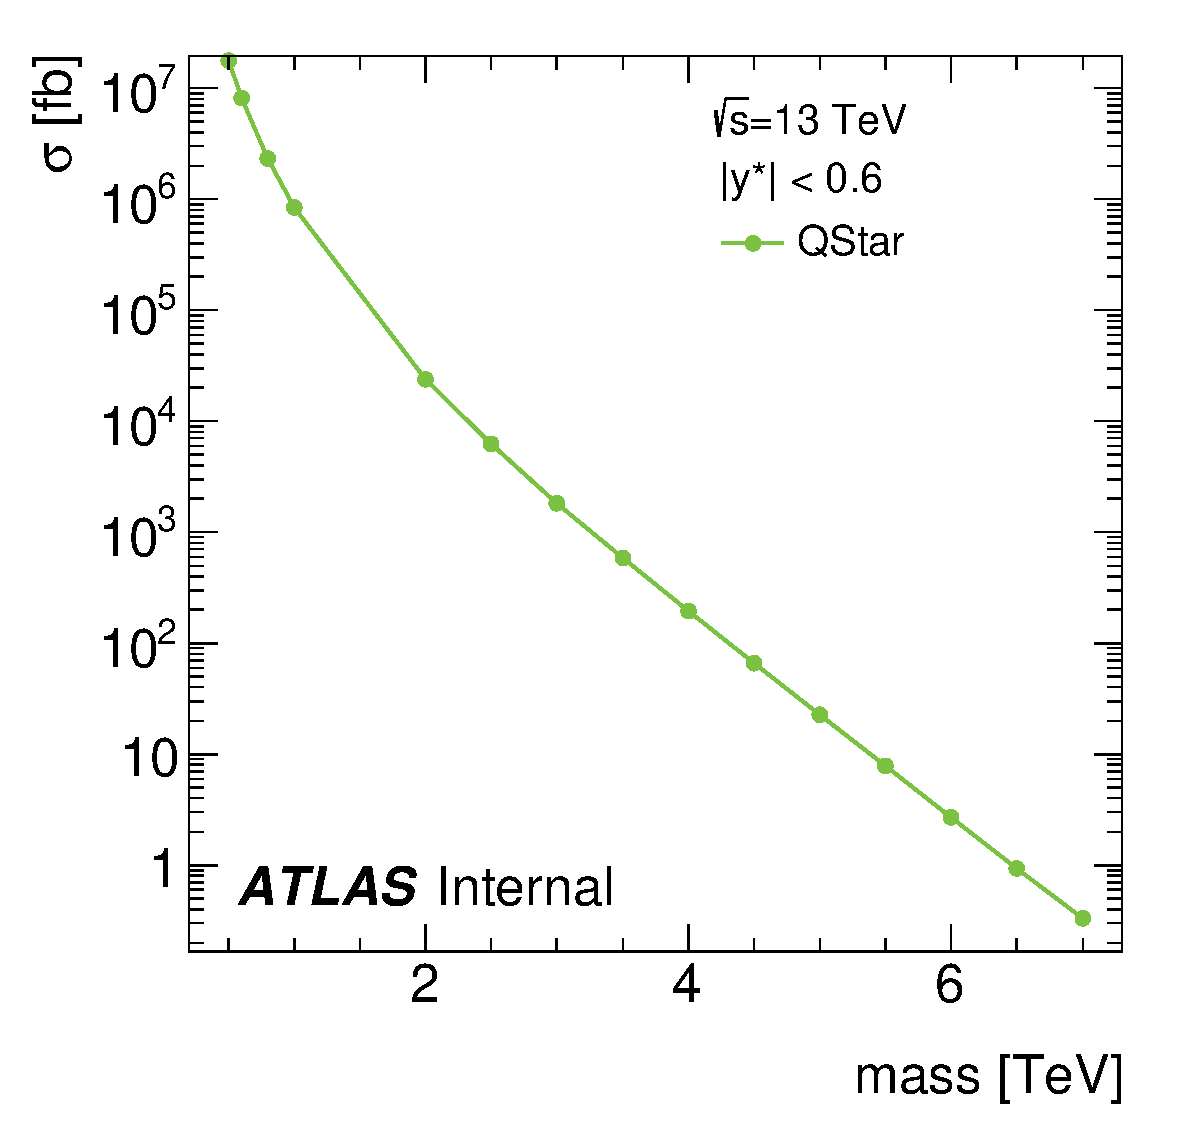
\includegraphics[width=0.48\textwidth]{figures/benchmark_signals/CrossSections_QStar_log} }
  \subfigure[Acceptance]{ \label{fig:acc} 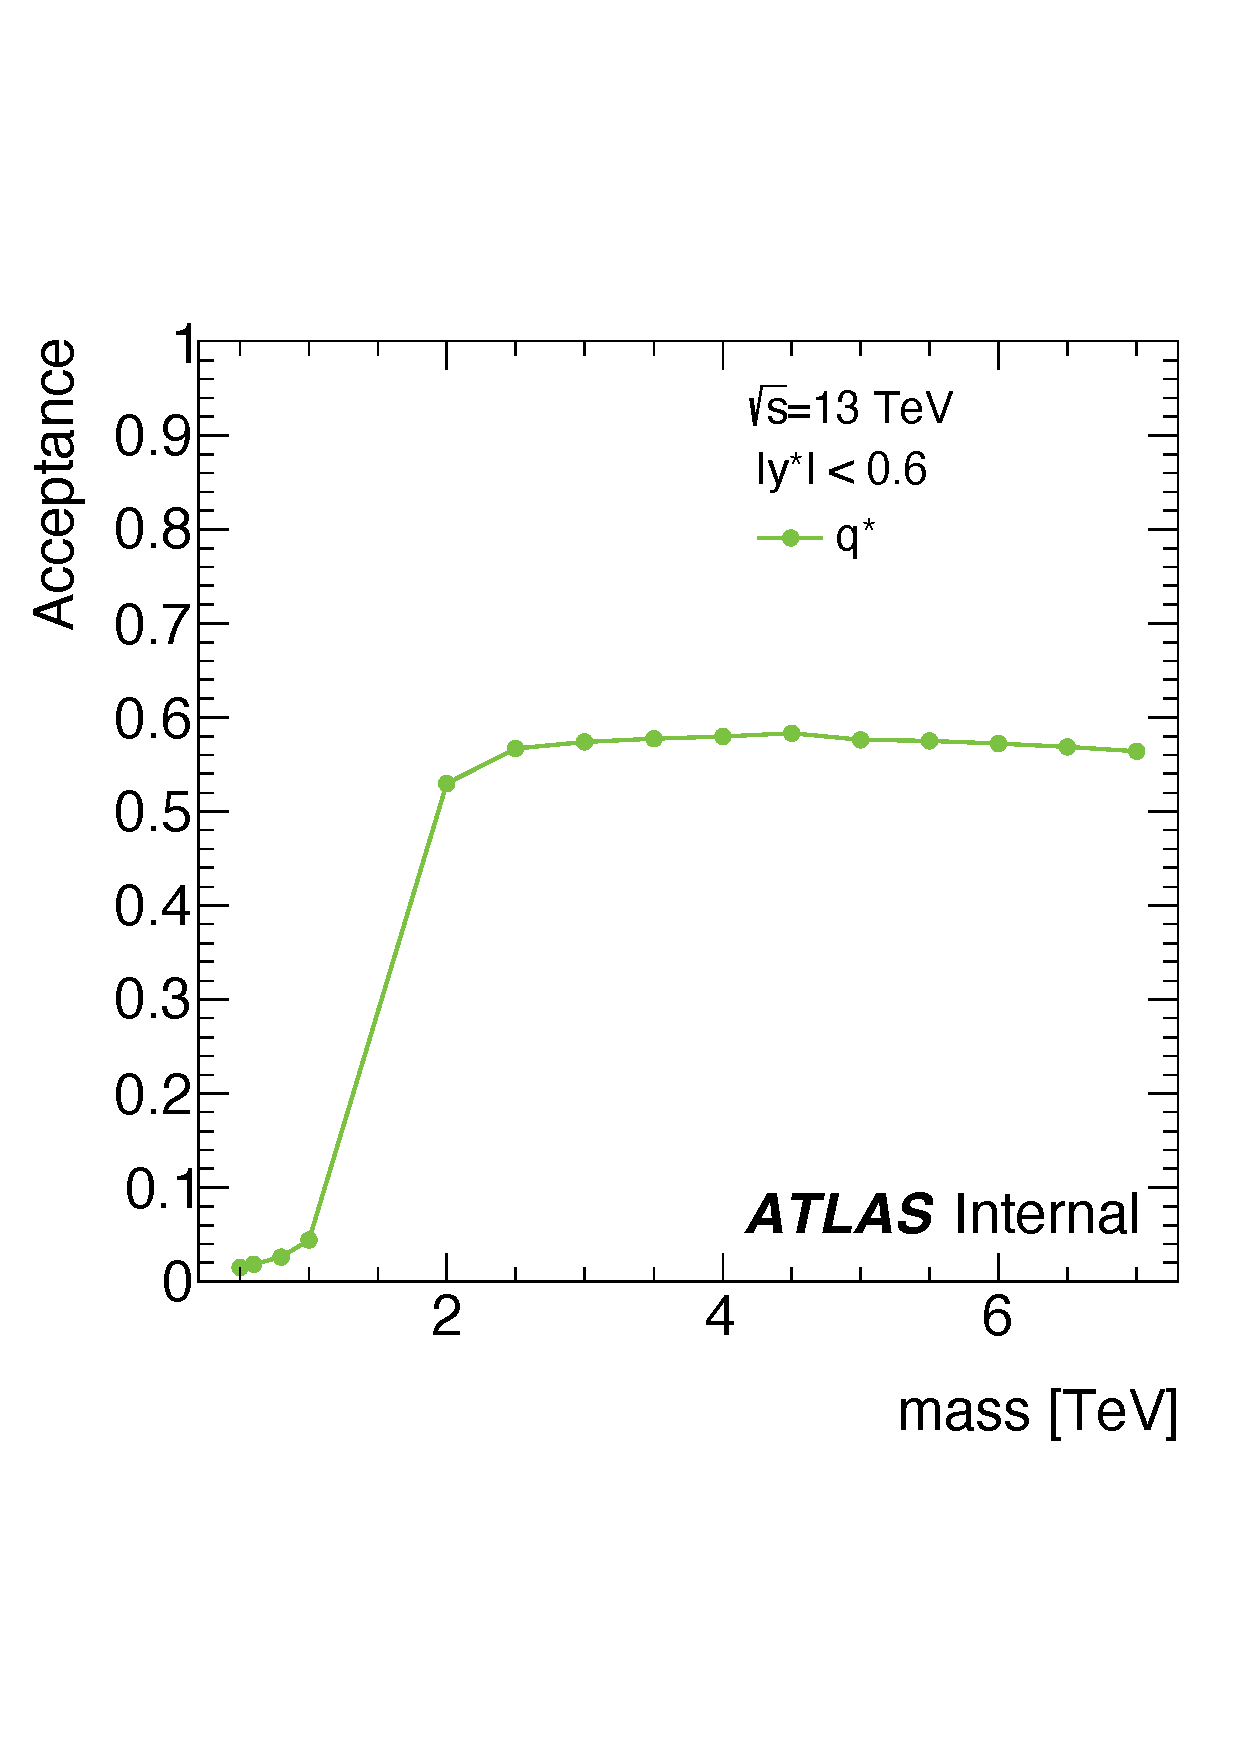
\includegraphics[width=0.48\textwidth]{figures/benchmark_signals/Acceptances_QStar} }
  \caption{(a) Cross section and (b) acceptance for the 
  light-flavored \qstar model for 13~\TeV~center-of-mass energies using the full resonance
  analysis selection (Section~\ref{sec:event_selection}).}
\end{figure}

\FloatBarrier
\end{comment}
\subsubsection{Quantum Black Holes}
%\label{sec:QBH} % uncomment if label used. 
%\todo{Do QBH decay to quarks or gluons, is there increased sensitivity or not} 
In our study, we employ the QBH model for the purpose of comparing limits with the previous iteration of the analysis. The feasibility of producing QBHs at the LHC is contingent upon the presence of sufficiently large extra dimensions within the universe. This model posits that the energy scale of quantum gravity $M_{D}$, at which QBHs are generated, diminishes as the number of these large extra dimensions, denoted as $n$, increases. Consequently, a larger $n$ permits lower mass scales at which QBHs can be formed.

Two-body isotropic final state is expected by the QBH decay at the LHC, where the $M_D$ energy threshold could be reached. Therefore the quantum gravitational effects can be probed by searches on \mjj spectrum. To simulate events involving quantum black holes with $n=6$, we utilize the \BlackMax~\cite{Dai:2007ki} Monte Carlo (MC) generator. This MC generator facilitates the simulation of QBH events within the $n=6$ framework..
%~\cite{Dai:2007ki}



%%%%%%%%%%%%%%%%%%%%%%%%%%%%%%%%%%%%%%%%%%%%%%%%%%%%%%%%%%%%%%%%%%%%%%%%%%%%%%%%%
%
%\clearpage
%\subsubsection{Signal shapes in the various models}
%
%The shape of the signal peak for each mass point and each signal model, after the resonance selection cuts, are shown in Figure~\ref{fig:showallshapes}. Each template is normalised to 1, and therefore differences in peak amplitude are indicative of a broadening or narrowing of the signal rather than of a change in cross section.
%\begin{figure}[!htb]
%\centering
%\subfigure[q* model]{\label{fig:resonance_templates_2500}
%               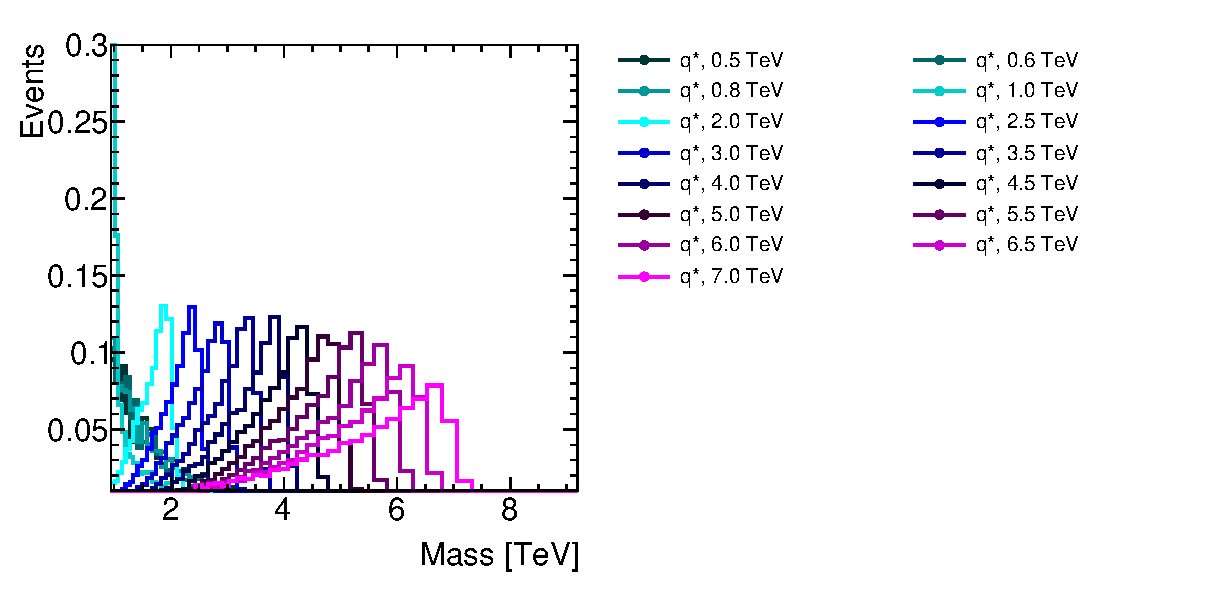
\includegraphics[height=0.25\textwidth]{figures/benchmark_signals/overlaidQStar_mjj_linear.eps}}
%\subfigure[\BlackMax\ model]{\label{fig:resonance_templates_4500}
%               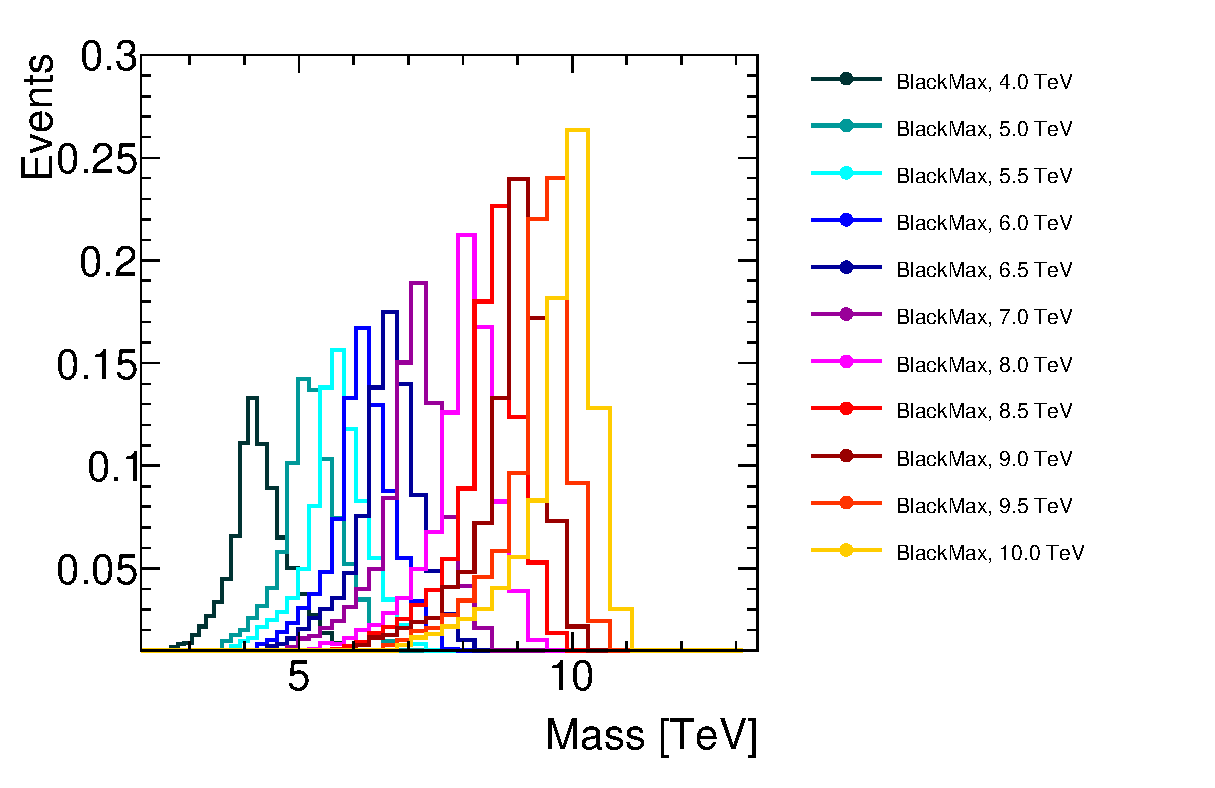
\includegraphics[height=0.25\textwidth]{figures/benchmark_signals/overlaidBlackMax_mjj_linear.eps}}
%\subfigure[\Wprime\ model]{\label{fig:resonance_tr_templates_2500}
%               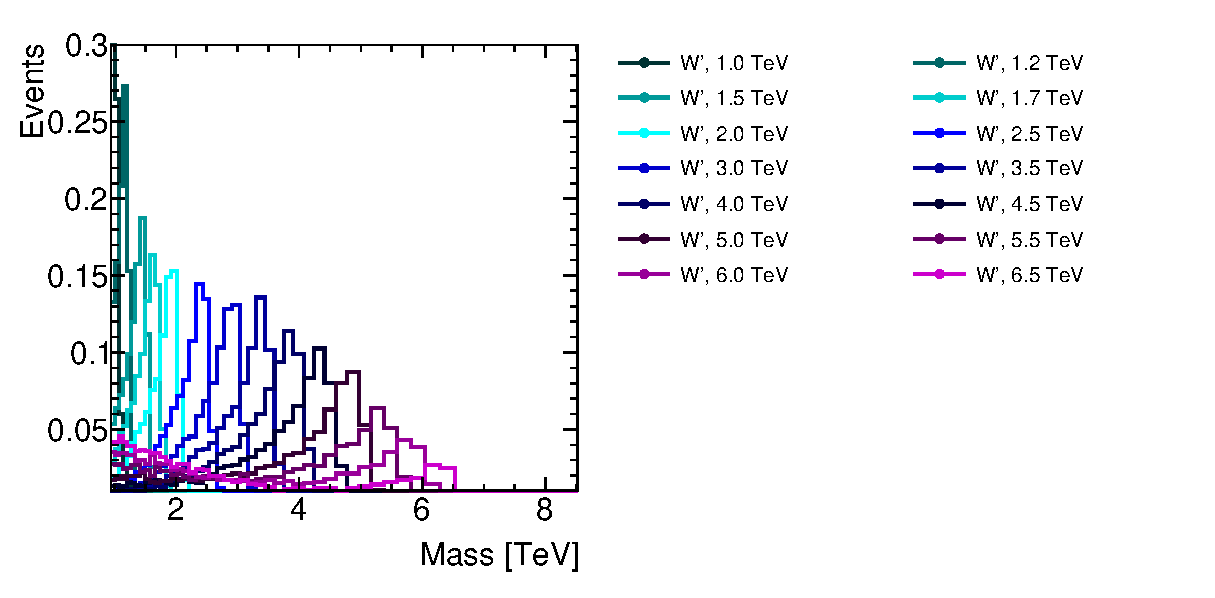
\includegraphics[height=0.25\textwidth]{figures/benchmark_signals/overlaidWPrime_mjj_linear.eps}}
%\subfigure[\Wstar\ model]{\label{fig:showallshapes}
%               \includegraphics[height=0.25\textwidth]{figures/Wstar/CrossAcceptance/MassesDist.pdf}}
%%\subfigure[4.5 TeV, truncated]{\label{fig:resonance_tr_templates_4500}
% %              \includegraphics[width=0.45\textwidth]{old_figures_2015/search_results/Resonance/Gaus_Comp/M4500_tr_comp.pdf}}
%\caption{Normalized \mjj\ templates at every mass point considered in the limit setting phasse for each of the resonant benchmark models. }
%
%\end{figure}
%

%This is demonstrated most clearly in Figure~\ref{fig:resonance_templates_shapes}, which shows overlaid reconstructed \mjj\ distributions for a selection of benchmark signals at the same mass point.
%The low-mass tail of \Wprime\ starts to become pronounced at higher masses, and the \qstar\ signal is also broadened. 
%In contrast to the previous two, 
%The detailed differences between the signal shapes become apparent in Figures~\ref{fig:resonance_tr_templates_4000} and \subref{fig:resonance_tr_templates_6500}, 
%which show the signal templates truncated at $\pm 20 \%$ of the generated mass. 
%This is the truncation recommended for recasting of the generic Gaussian observed limits set by this analysis into signals with peaked but non-Gaussian \mjj\ distributions. 
%The truncated distributions show that the \qstar\ signal distributions are shifted the most to lower \mjj\ of all signals, for both lower and higher masses. 
%% 
%% 
%\begin{figure}[!htb]
%\centering
%\subfigure[4.0 TeV]{\label{fig:resonance_templates_4000}
%               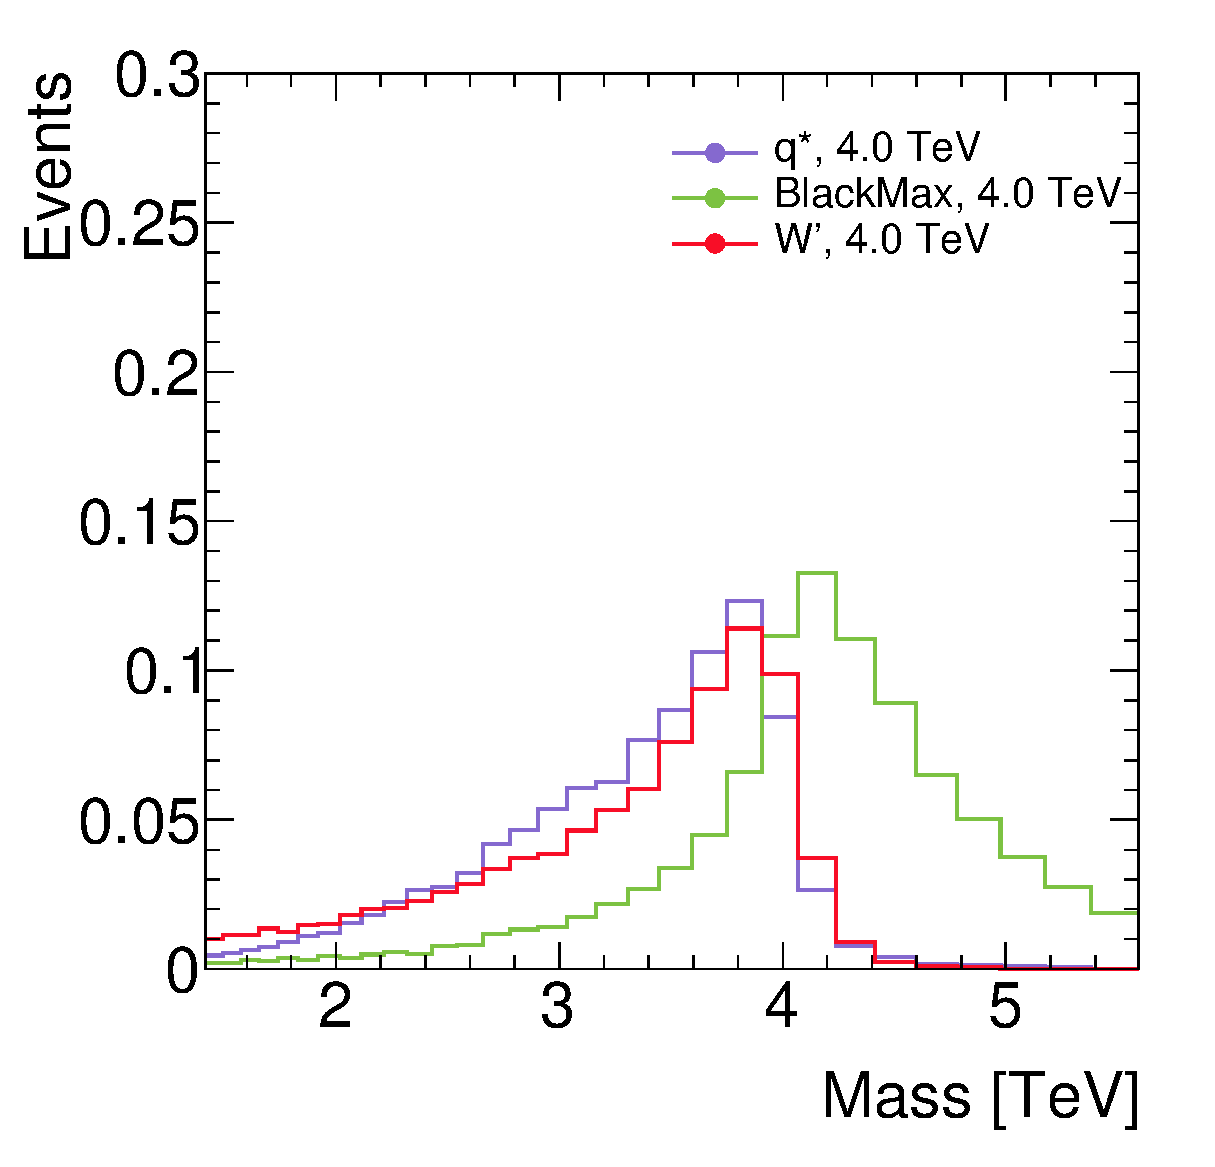
\includegraphics[width=0.45\textwidth]{figures/benchmark_signals/overlaidSignals_m4000_linear.eps}}
%\subfigure[6.5 TeV]{\label{fig:resonance_templates_6500}
%               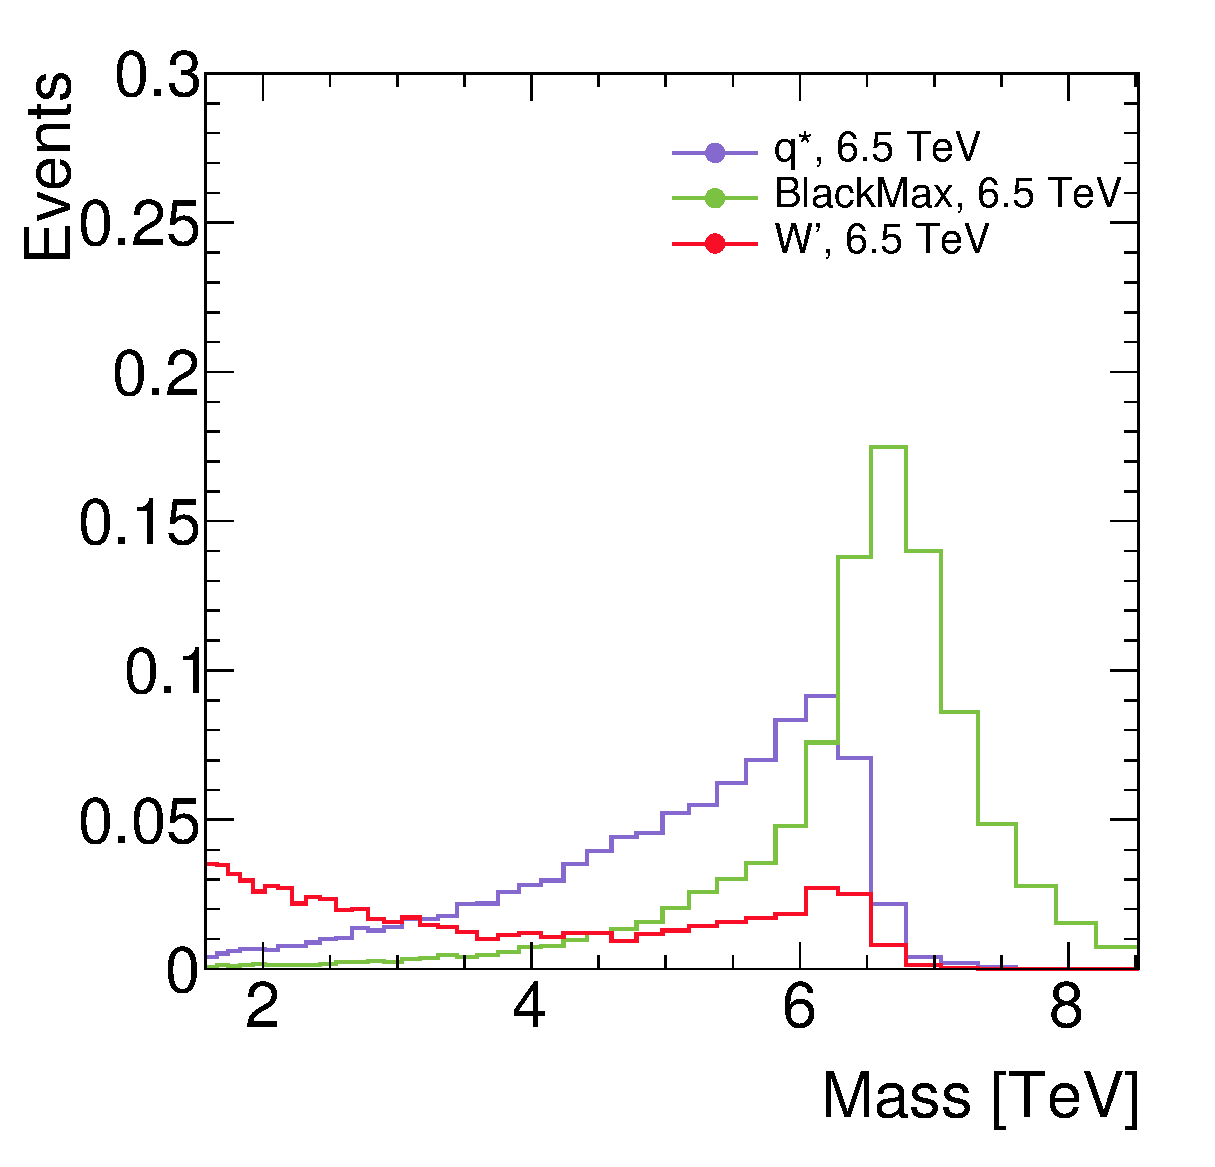
\includegraphics[width=0.45\textwidth]{figures/benchmark_signals/overlaidSignals_m6500_linear.eps}}
%\subfigure[4.0 TeV, truncated]{\label{fig:resonance_tr_templates_4000}
%               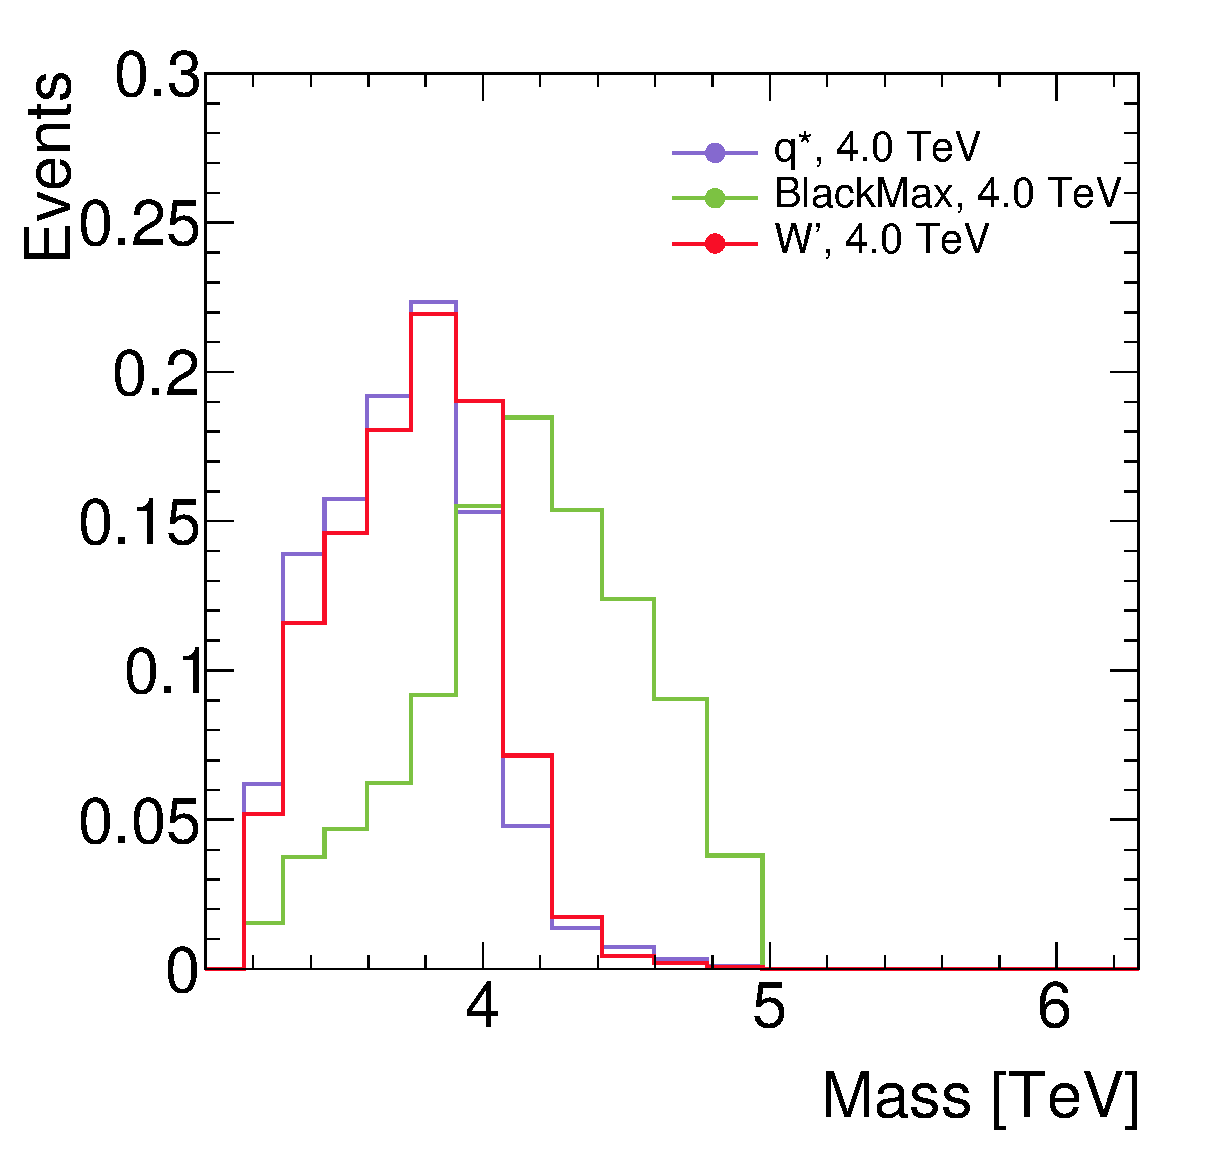
\includegraphics[width=0.45\textwidth]{figures/benchmark_signals/overlaidSignals_m4000_trunc.eps}}
%\subfigure[6.5 TeV, truncated]{\label{fig:resonance_tr_templates_6500}
%               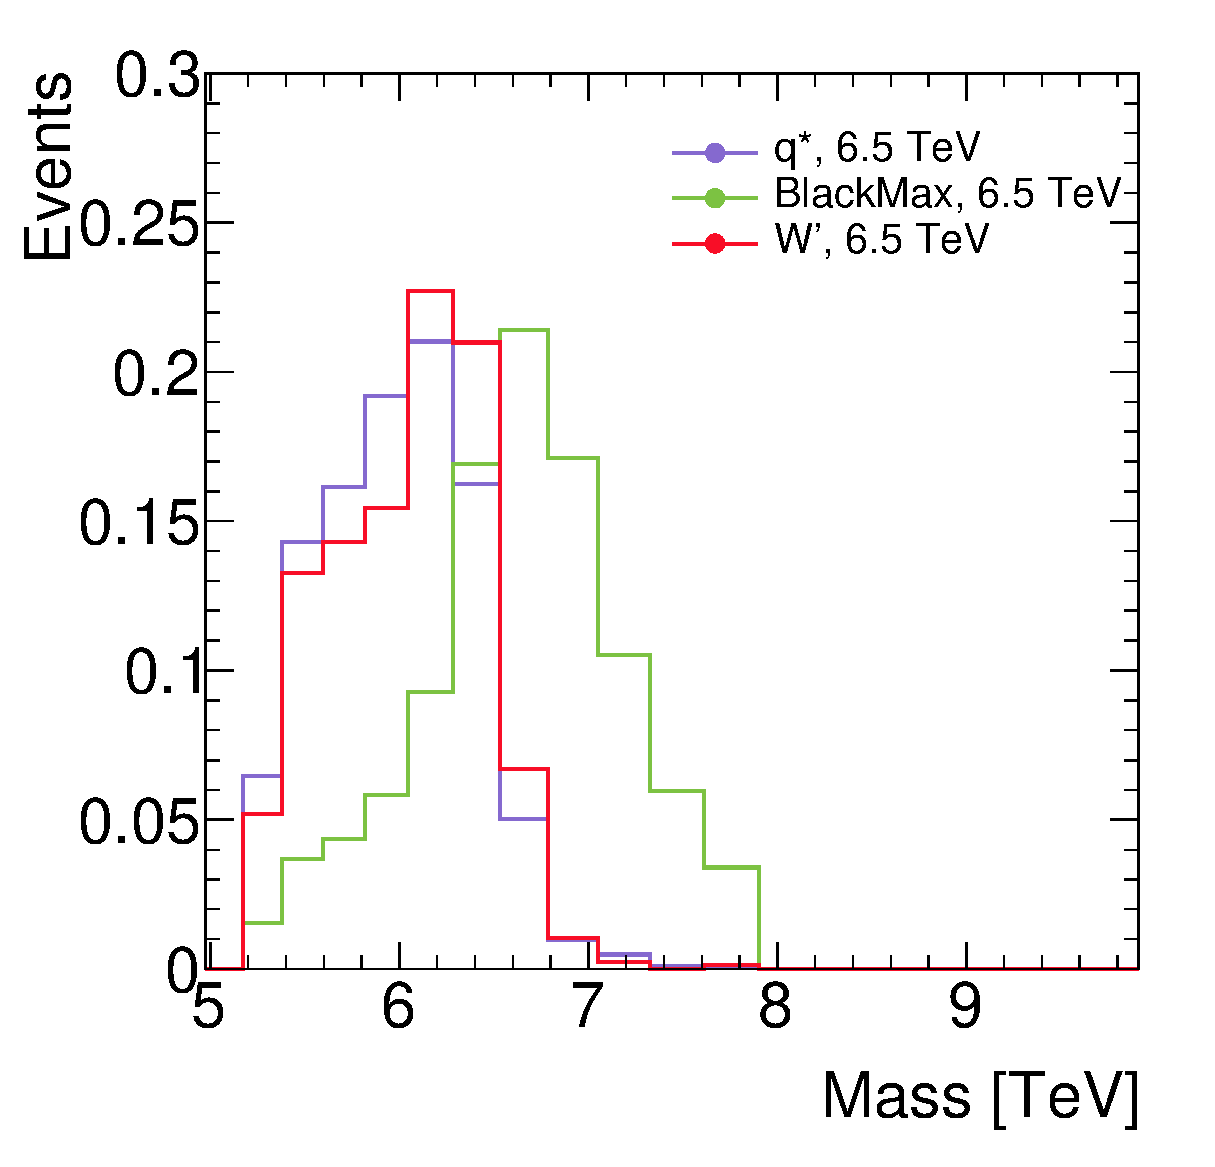
\includegraphics[width=0.45\textwidth]{figures/benchmark_signals/overlaidSignals_m6500_trunc.eps}}
%
%\caption{Normalized \mjj\ templates at 4.0 TeV \subref{fig:resonance_templates_4000},\subref{fig:resonance_tr_templates_4000} and 6.5 TeV \subref{fig:resonance_templates_6500},\subref{fig:resonance_tr_templates_6500}, before (above) and after (below) the truncation procedure, for various resonant benchmark models. The signals are re-normalised after truncation for ease of comparison of the shapes.}
%\label{fig:resonance_templates_shapes}
%\end{figure}
%

%\clearpage
%%%%%%%%%%%%%%%%%%%%%%%%%%%%%%%%%%%%%%%%%%%%%%%%%%%%%%%%%%%%%%%%%%%%
%\subsubsection{Signal Morphing}
%\label{sec:SwiftMorphing}
%%%%%%%%%%%%%%%%%%%%%%%%%%%%%%%%%%%%%%%%%%%%%%%%%%%%%%%%%%%%%%%%%%%%

%\todo[inline] {Will we use morphing?}


%Smooth signal mass distributions are obtained  from morphing the signal shapes from MC. The MC signals are fit to a Gaussian + reverse Landau function, a parameterization that has one normalization and five shape parameters. The parameters are interpolated as a function of mass using cubic splines. This allows the use of signal shapes at any mass. Figure~\ref{fig:morphing} shows some examples of fits to MC signal shapes as well as several interpolated signal shapes.  
%
%\begin{figure}[!htb]
%	\centering
%	\subfigure[q* signals]{ \includegraphics[width=0.48\textwidth]{figures/SWiFt/interpolate_qStar.pdf} }
%	\subfigure[Reclustered W' signals]{ \includegraphics[width=0.48\textwidth]{figures/SWiFt/interpolate_WPrimeRe.pdf} }
%	\subfigure[Z' 0.2 SM coupling signals]{ \includegraphics[width=0.48\textwidth]{figures/SWiFt/ZPrime_gSM0p20.pdf} }
%	\subfigure[Z' 0.5 SM coupling signals]{ \includegraphics[width=0.48\textwidth]{figures/SWiFt/ZPrime_gSM0p50.pdf} }
%	\caption{
%		Signal morphing for some MC signals. The solid colored histograms are MC signal shapes and the dotted lines of the same color are fit to the MC shapes. The dotted pink curves are the morphed shapes.  
%		\label{fig:morphing}}
%\end{figure}
%
%To stress test the morphing technique, tests were done where the a set of mass MC signal shapes were removed and the morphing was done with the remaining shapes. The results of this test is shown in figure~\ref{fig:morphingTest}, where in (a) integer MC q* shapes (2 \TeV\ , 3 \TeV\ , 4 \TeV\ , 5 \TeV\ , 6 \TeV\ ) are removed and morphing is done using the odd shapes only and in (b) fractional MC shapes (2.5 \TeV\ , 3.5 \TeV\ , 4.5 \TeV\ , 5.5 \TeV\ ) are removed and the even shapes are used for morphing. The technique recovers the shapes of the removed signals fairly well.  
%
%\begin{figure}[!htb]
%	\centering
%	\subfigure[q* signals. Morphing with odd masses only.]{ \includegraphics[width=0.48\textwidth]{figures/SWiFt/interpolateWorking_evenRemoved.pdf} }
%	\subfigure[q* signals. Morphing with even masses only.]{ \includegraphics[width=0.48\textwidth]{figures/SWiFt/interpolateWorking_oddRemoved.pdf} }
%	\caption{
%		Signal morphing stress test. (a) Even mass signals are removed and morphing is done with odd masses only. (b) Odd mass signals are removed and morphing is done with even masses only. 
%		\label{fig:morphingTest}}
%\end{figure}  
%



\clearpage

\subsection{Events selections}
\label{sec:event_selection}
The MC and data events are divided into three categories to perform the search: the untagged dijet invariant mass spectrum, one-gluon tagged spectrum, and two-gluon tagged spectrum. The evidence of BSM resonances would appear as peaks in the \mjj~spectrum formed by two highest \pt~jets in the events. A series of specific cuts is applied to improved the sensitivity of the searches.


\subsubsection{Observables and Kinematic Variables}
%\label{sec:observables}
The predominant source of dijet
events in the SM is two-to-two scattering though the QCD processes. This search exams two key properties of the QCD background:
\begin{itemize}
	\item The background at high \mjj~appears as a smooth and continuously falling spectrum.
	\item The background at high energy strongly peaks in the forward region as a result of Rutherford $t$- and $u$-channel poles in the cross sections
for certain scattering processes \cite{Harris:2011bh}.
\end{itemize}

Resonances of interest have $\cos{\theta}$ distributions in the detector, which in contrast to Rutherford scattering, are either isotropic or have polynomial behaviour in $\cos{\theta}$~\footnote{See Ref.~\cite{Harris:2011bh} p15 for a summary.}, thus a angular distribution appears. This search therefore defines a \ystar to indicate the angle separation of the jets in the selected events:
\begin{equation}
 \ystar = (y_1-y_2)/2
\end{equation}
to improve the sensitivity to higher energies where new phenomena are expected. The variables $y_1, y_2$ represent the rapidity of the leading and subleading jet. The value of the \ystar\ cut on events is optimized for each signal as discussed in Section~.\ref{section:ystarCutOptimization}.


In this analysis, jets are reconstructed with the \akt~algorithm
% \cite{Cacciari:2008gp}
with a radius parameter R = 0.4, as implemented in the \textsc{FastJet}
package~\cite{Cacciari:2011ma}.  The EMTopo jets, reconstructed from topological clusters via procedures described in Section.~\ref{sec:4.1}, are used. The standard \textit{Loose} cut is applied to jet quality as well as jet cleaning. The summarized jet criteria are shown in Table~\ref{tab:jetCalibration}.

\begin{table}[ht]
	\centering
		\begin{tabular}{clc}
			\hline
			Parameter / Observable & Requirement \\
			\hline
			Algorithm & \akt \\
			R-parameter & 0.4 \\
			Input Constituent & EMTopo\\
			\pt & $>$150 GeV \\
			\textbar$\eta$\textbar & $<$2.1 \\
			\hline
	\end{tabular}
\caption{Jet selection criteria used in this analysis.}
\label{tab:jetCalibration}
\end{table}


\subsubsection{Baseline selection}
\label{sec:base_selection}


The triggers used in this analysis is HLT\_j420. Besides, two single-jet trigger HLT\_j225\_gsc420\_boffperf\_split is also used as the unprescaled trigger for full Run 2 data. Both triggers have the threshold of $\pt > 420$ GeV of the jets, while the GSC is applied to the HLT\_j225\_gsc420\_boffperf\_split to the trigger turn-on improvement. A turn-on based on the \mjj~spectrum is found to be much powerful than the cut requirement of the leading jet \pt, where the \mjj~cut imposes a soft cut on the leading and subleading jet, respectively~\cite{Nishu:2646455}. More details are shown in Section.~\ref{section:dijetmassturn-on}. 



%The two triggers were found to be very similar in performance in Ref.~\cite{Nishu:2646455}; we used HLT\_j420 trigger. It was also found in Ref.~\cite{Nishu:2646455} that obtaining the turn-on directly from \mjj\ provides a much power turn-on than from requiring a specific cut on the leading jet \pT\.

The baseline event selection is applied for all categories. The GRL and various flags that indicate the status of detector when taking data are provided by the ATLAS Data Quality (DQ) group, are applied to ensure the data integrity. Primary vertex requirement is also included to ensure good quality jets. The  


\begin{itemize}
\item All jets with $\pt > 150$ GeV pass \textit{Loose} cleaning cuts
\item Passes the lowest unprescaled single-jet trigger: HLT\_j420
\item Jet multiplicity $\ge 2$
\item Leading jet $\pt > 380$ GeV and subeading jet $\pt > 150$ GeV
\item Leading jet \abseta~< 2.1 and subeading jet \abseta~< 2.1 
\item $|\Delta\phi|$ between two jets: $|\Delta\phi| > 1.0$
\item \mjj > 1100 GeV
\end{itemize}

Additional kinematic criteria are applied according to the distributions of signals, in order to optimize the
search potential, are then discussed in Section~\ref{section:ystarCutOptimization}.



\begin{comment}
\subsection{Analysis cutflow}
%\label{sec:data_cutflow}

This section and the next present the analysis cutflows. Cutflows obtained on
Run~2 data are presented in Tables~\ref{tab:cutFlow_resonance_run2} and 
\ref{tab:cutFlow_wstar_run2}.

\begin{table}[htbp]
	\centering
	\begin{tabular}{l|c|c}
		\hline\hline
		Selection criteria & $N_{events}$ & rel. decrease (\%) \\
		\hline
		all      &	4738142726	&	0.00	\\
		Apply GRL 	& 	4442605390        & 	-6.24	 \\
		Cleaning	 & 	4379077017	 & 	-1.43	 \\
		HLT j420	 & 	266104885	 & 	-93.9	 \\
		jet pre-selection	 &     259157844         &      -2.61    \\
		$|\Delta\phi| > 1.0$	 & 		 & 		 \\
		$|\ystar| < 0.6$	 & 		 & 		 \\
		$\mjj>1100~\GeV$	 & 		 & 		 \\
		\hline\hline
	\end{tabular}
	\caption{Cutflow for
		events with H$^\prime$ cuts:  $\mjj>1100~\GeV$, and $|\ystar|<0.6$. .
		\label{tab:cutFlow_resonance_run2} }
\end{table}

\begin{table}[htbp]
	\centering
	\begin{tabular}{l|c|c}
		\hline\hline
		Selection criteria & $N_{events}$ & rel. decrease (\%) \\
		\hline
		all      &	4738142726	&	0.00	\\
		Apply GRL 	& 	4442605390        & 	-6.24	 \\
		Cleaning	 & 	4379077017	 & 	-1.43	 \\
		HLT j420	 & 	266104885	 & 	-93.9	 \\
		jet pre-selection	 &     259157844        &      -2.61    \\
		$|\Delta\phi| > 1.0$	 & 		 & 		 \\
		$|\ystar| < 0.8$	 & 		 & 	 \\
		$\mjj>1133~\GeV$	 & 		 & 	 \\
		\hline\hline
	\end{tabular}
	\caption{Cutflow for
		events with string resonance cuts:  $\mjj>1133~\GeV$, and $|\ystar|<0.8$. .
		\label{tab:cutFlow_wstar_run2} }
\end{table}
\end{comment}

\clearpage


\subsection{Quark-Gluon sample selection}
\label{sec:QGselection}.  % uncomment if label used. 
The sensitivity of the search on the resonant is expected to increase by distinguishing the type of parton that initiated the jets. The parton types of dijet events as a function of \mjj from the MC with a  \textsc{Pythia8.186} at LO  NNPDF2.3 PDFs is shown in Figure~\ref{fig:quarkgluonfraction}, suggesting that the search for new resonance can be improved by tagging quark and gluon jets.

%ATLAS has published a study \cite{ATL-PHYS-PUB-2017-009} 

In this section we present the search for new particles using the full Run~2 $\sqrt{s} = 13$~TeV\xspace dataset with quark and gluon tagging method.


\begin{figure}[htb]
 \centering
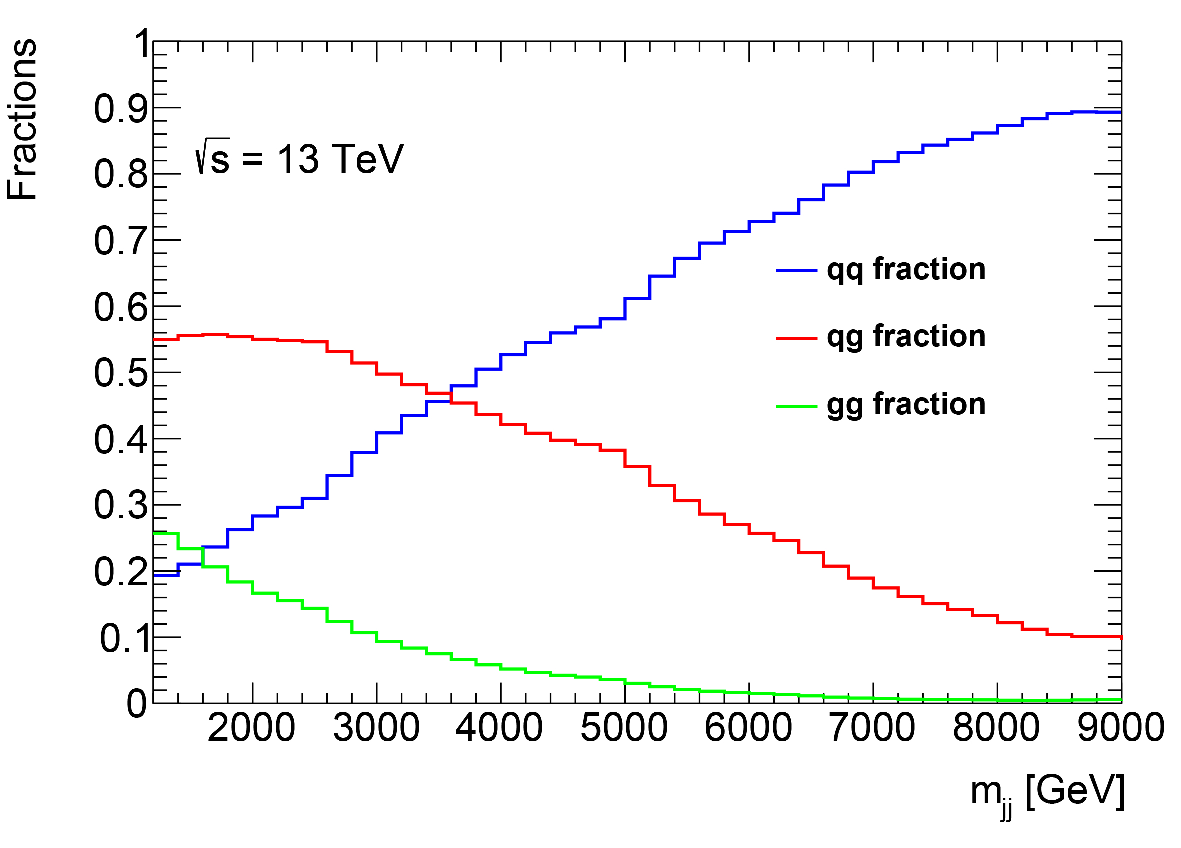
\includegraphics[width=0.75\textwidth]{fig/tagging/Fractions_QCD.pdf}
\caption{The fraction of dijet events that are initiated by quark-quark events (blue), quark-gluon 
events (green) and gluon-gluon events (red) in simulated data.  \label{fig:quarkgluonfraction}}
\end{figure}


Previous study in ATLAS has shown that the jets can be tagged quark or gluon jets based on the number of charged tracks associated with the jets with \pt~above 500 MeV. Samples with enhanced fractions of quark or gluon initiated jets can be created by using a selection based on the charged-particle constituent multiplicity \ntrk. As shown in Fig.~\ref{fig:jet_pt_quark_gluon}, where \pythia8 generator~is used for MC to ensure a good agreement with the distribution of \ntrk~in data within the ID acceptance $|\eta|<2.1$.

\begin{figure}[htb]
 \centering
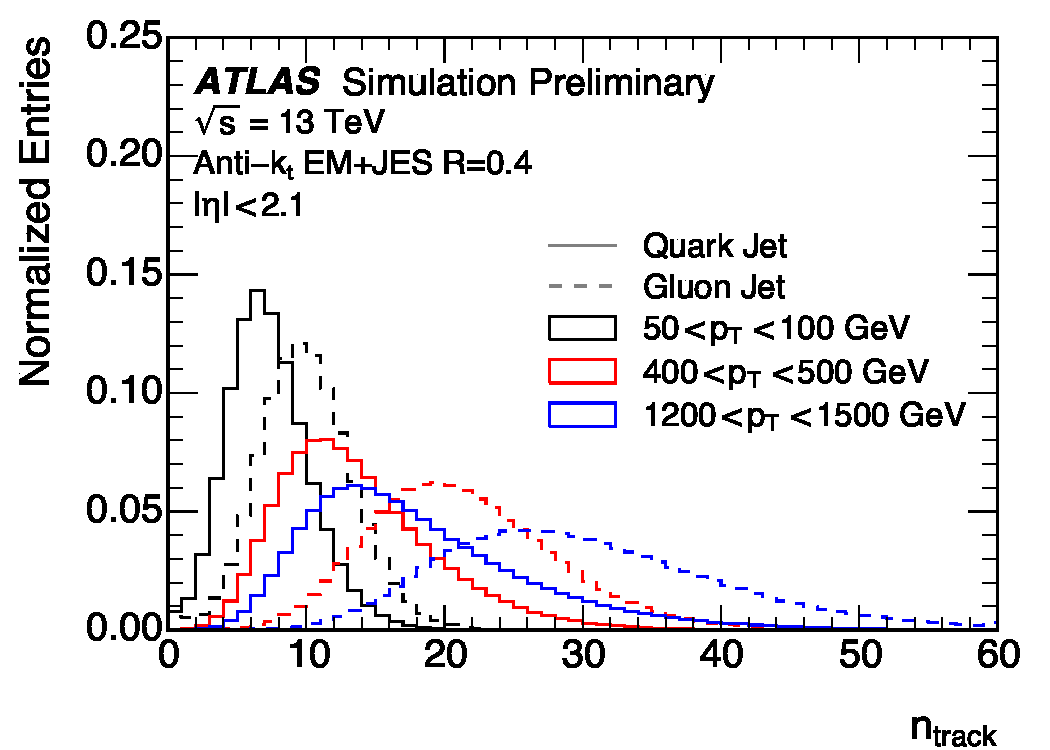
\includegraphics[width=0.65\textwidth]{fig/tagging/fig_01_ATL-PHYS-PUB-2017-009.pdf}
\caption{Distribution of the jet reconstructed track multiplicity (\ntrk ) in
 different \pt\ ranges with the \pythia~8 MC samples and processes with a full simulation of the
 ATLAS detector. Tracks are required to have $\pt~> 500$ MeV and pass
  quality criteria described in Ref.~\cite{ATL-PHYS-PUB-2017-009}. }
\end{figure}


\subsubsection{Expected Signal Significance}
%\label{sec:ExpectedSig}

The shape of \mjj from QCD is complex and rapidly changing according to the fractions of events that originate from quark-quark, quark-gluon and gluon-gluon scattering. The QCD background is presented in Section~\ref{qcdsamps}. The MC simulated signals and background is thus used for estimating the expected signal significance.


\paragraph{Resonances that decay to quark-quark\\}

The statistical significance associated with signals decaying into quark-antiquark pairs is assessed using \Zprime\ models using 
\begin{equation}
	S = N_S \sum_i{ \dfrac{ f_{qq,i}\epsilon_{qQ}^2 + f_{qg,i}\epsilon_{qQ}\epsilon_{gQ} + f_{gg.i}\epsilon_{gQ}^2  } {\sqrt{ B_{qq,i}\epsilon_{qQ}^2 + B_{qg,i}\epsilon_{qQ}\epsilon_{gQ} + B_{gg,i}\epsilon_{gQ}^2  }}}
\end{equation}
where $N_S$ is the number of signal events, $f_{qq,i}$ is fraction of signal events that result in the two 
highest \pT\ jets that where initiated by quarks in bin $i$ ( $f_{qg,i}$ are quark-gluon jets, and $f_{gg,i}$ is two gluon jets), 
$\epsilon_{qQ}$ is the efficiency of a quark initiated jet passing the quark selection criteria, 
$\epsilon_{gQ}$ is the efficiency of a gluon initiated jet passing the quark selection criteria, 
and $B_{xx,i}$ is the expected number of background events with quark-quark, quark-gluon or gluon-gluon initiated jets. 


The statistical significance is computed for \Zprime\ particles mass values within the range of 1500 to 4000 GeV, and for quark-jet selection efficiencies ranging from 30\% to 90\%. The obtained significance values are presented in Figure~\ref{fig:QuarkSignalSignificance}. The depicted results illustrate a trend of diminishing significance when any quark-selection criteria is imposed on the data. This decline in significance can be attributed to the dominant presence of quark-quark events within the data, where the selection process concurrently diminishes both background and signal contributions to a comparable extent.

\begin{figure}[htb]
	\centering
	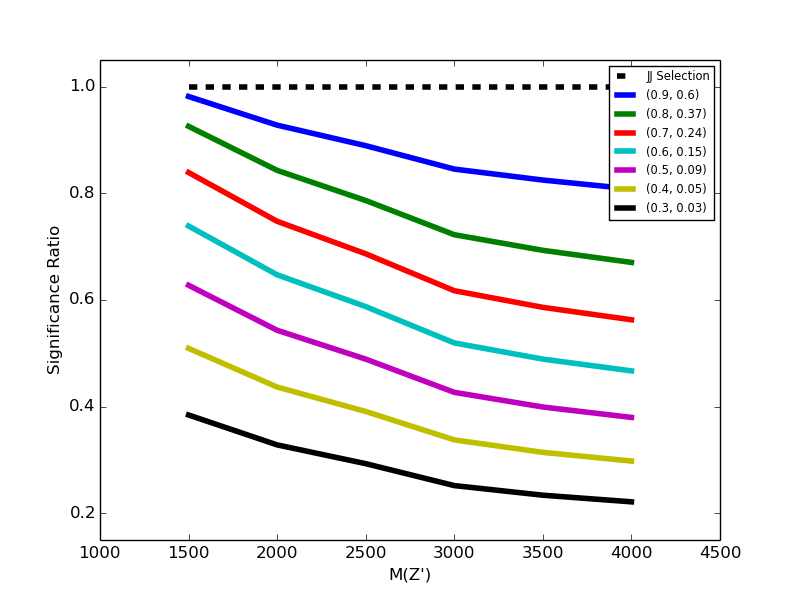
\includegraphics[width=0.75\textwidth]{fig/tagging/QuarkSignalSignificance.png}
	\caption{ The significance for observing a \Zprime\ with masses from 1500 to 4000 GeV
		for $\epsilon_{qQ}$ ranging from 90 to 30\% compared to the significance calculated with no quark selection applied. The key gives pairs of efficiencies ($\epsilon_{qQ}$, $\epsilon_{gQ}$).
		\label{fig:QuarkSignalSignificance}}
\end{figure}


\paragraph{Signals that decay to gluon-gluon\\}
The significance for signals that decay to a gluon-gluon pair are using \Hprime\ models, estimated by:
\begin{equation}
S = N_S \sum_i{ \dfrac{ f_{qq,_i}\epsilon_{qG}^2 + f_{qg,i}\epsilon_{qG}\epsilon_{gG} + f_{gg,i}\epsilon_{gG}^2  } {\sqrt{ B_{qq,i}\epsilon_{qG}^2 + B_{qg,i}\epsilon_{qG}\epsilon_{gG} + B_{gg,i}\epsilon_{gG}^2  }}}
\end{equation}
where  
$\epsilon_{qG}$ is the efficiency of a quark initiated jet passing the gluon selection criteria, 
$\epsilon_{gG}$ is the efficiency of a gluon initiated jet passing the gluon selection criteria. 

The computation of significance involves the utilization of simulated \Hprime signals, with masses ranging from 2000 to 7000 GeV. The efficiencies of gluon tagged are varied across from 60\% to 90\%. The resulting significances, depicted as functions of \Hprime masses, are presented in Figure~\ref{fig:GluonSignalSignificance}. The observed trend reveals a gradual increase in significance, with values ascending from approximately 1.2 at 2 TeV to around 1.6 at 7 TeV. Notably, the most substantial enhancements occur at a gluon efficiency of 75\%.


\begin{figure}[htb]
 \centering
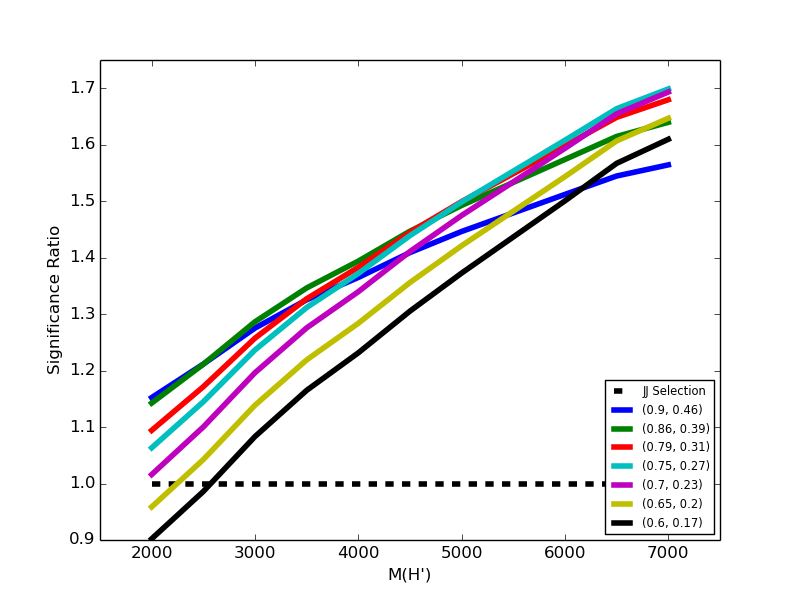
\includegraphics[width=0.75\textwidth]{fig/tagging/GluonSignalSignificance.png}
\caption{ The significance for observing a \Hprime\ with masses from 2000 to 7000 GeV
for $\epsilon_{gG}$ ranging from 90 to 60\% compared to the significance calculated with no gluon selection applied. The key gives pairs of efficiencies ($\epsilon_{gG}$, $\epsilon_{qG}$).
  \label{fig:GluonSignalSignificance}}
\end{figure}


\paragraph{Signals that decay to quark-gluon\\}

Calculating the significance for signals involving quark-gluon decays, such as string decays, poses increased complexity due to the potential overlap in the selection criteria between decaying jets that satisfy both quark and gluon criteria. In this context, it becomes imperative to establish distinct efficiencies exclusively tailored for quark- and gluon-jets. Thus the efficiencies are needed to be defined exclusively for quark- and gluon-jets.

The efficiencies for quark-jets are defined as:

\begin{itemize}
\item $\epsilon_{qQ}$ The efficiency that a quark-jet is identified only as a quark-jet. 
\item $\epsilon_{qQG}$ The efficiency that a quark-jet is identified as a quark- and a gluon-jet.
\item $\epsilon_{qG}$ The efficiency that a quark-jet is identified only as a gluon-jet.  
\end{itemize}
where $\epsilon_{qQ} + \epsilon_{qQG} + \epsilon_{qG} = 1$. 

Another set of efficiencies that is measured for gluon-jets are:
\begin{itemize}
\item $\epsilon_{gQ}$ The efficiency that a gluon-jet is identified only as a quark-jet. 
\item $\epsilon_{gQG}$ The efficiency that a gluon-jet is identified  as a quark- and a gluon-jet.
\item $\epsilon_{gG}$ The efficiency that a gluon-jet is identified only as a gluon-jet.  
\end{itemize}

The probability of truth pairs of quark-quark ($p_{qq}$), quark-gluon ($p_{qg}$) and gluon-gluon ($p_{gg}$) events that passing the quark-gluon tagging selection criteria are given by:
\begin{align}
p_{qq} & = 2  \epsilon_{qQ}\epsilon_{qG} + \epsilon_{qQG}\left( \epsilon_{qQ} + \epsilon_{qG} \right)  + \epsilon_{qQG}\epsilon_{qQG} \\
p_{gg} & = 2  \epsilon_{gQ}\epsilon_{gG} + \epsilon_{gQG}\left( \epsilon_{gQ} + \epsilon_{gG} \right)  + \epsilon_{gQG}\epsilon_{gQG} \\
p_{qg} & = \epsilon_{qQ}\epsilon_{gG} + \epsilon_{gQ}\epsilon_{qG} + \epsilon_{qQG}\left( \epsilon_{gQ} + \epsilon_{gG} \right) 
+ \epsilon_{gQG}\left( \epsilon_{qQ} + \epsilon_{qG} \right) 
+ \epsilon_{gQG}\epsilon_{gQG}
\end{align}
the related significance is then defined as:
\begin{equation}
S = N_S \sum_i{ \dfrac{ f_{qq,i} p_{qq} + f_{qg,i}p_{qg} + f_{gg,i}p_{gg}  } {\sqrt{ B_{qq,i}p_{qq} + B_{qg,i}p_{qg} + B_{gg,i}p_{gg}  }}}.
\end{equation}

No obvious benefit is observed after applied a quark selection with selection efficiencies from 30 to 100\%. A small but significant improvement is obtained in significance by applying a gluon selection to one of the two leading jets.
The resulting significances are  in Fig.~\ref{fig:QuarkGluonSignalSignificance} where an increase of 25\% in significance at masses above 5 TeV is obtained, with the largest increases happening over 70\% gluon efficiency.

\begin{figure}[htb]
 \centering
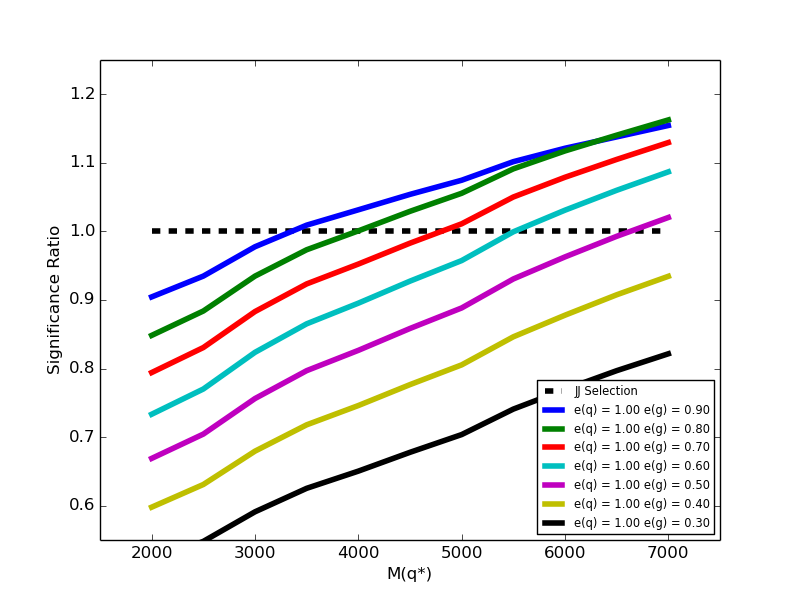
\includegraphics[width=0.75\textwidth]{fig/tagging/QuarkGluonSignalSignificance3.png}
\caption{ The significance for observing a \qstar\ with masses from 2000 to 7000 GeV 
for $\epsilon_{gG}$ ranging from 30 to 90\% compared to the significance calculated with no gluon selection applied. The key gives pairs of efficiencies ($\epsilon_{gG}$, $\epsilon_{qG}$).
  \label{fig:QuarkGluonSignalSignificance}}
\end{figure}

\FloatBarrier

\subsubsection{Selection Criteria}

The selection criteria for an quark-enriched jet sample was chosen so that 60\% quark-initiated purity is achieved in each jet \pt~bin. However, discontinuities in the \mjj spectrum would occur when such criteria is applied to the high mass (\pt~> 5000 GeV), leads to difficulties presented in resonance search. 


A selection criteria is thus built as a linear function of the $\ln(\pt) $, results in a smooth \mjj distribution. A jet is tagged as being more likely to be quark-initiated if \ntrk~is less than
the threshold \nq and more likely to be gluon-initiated if \ntrk~is 
greater than the threshold \ngluon: 
\begin{align}
\ntrk & \le \nq \; \mbox{quark-initiated sample} %\label{eq:QGselect}  % uncomment if label used. 
\\
\ntrk	  & \ge \ngluon \; \mbox{gluon-initiated sample} \nonumber
\end{align}
where   
\begin{equation}
n_{\mathrm{q(g)}} = {c_{\mathrm{q(g)}} + m_{\mathrm{q(g)}} \ln(\pt)}  \label{eq:nqg2}
\end{equation}
parameters $m_{\mathrm{q(g)}}$ and $c_{\mathrm{q(g)}}$ are constants obtained from the MC samples, these are founded by  finding the value of \ntrk\ 
that corresponds to a given efficiency for truth quark and gluon jets in 
\pt~bins, and chosen to defined suitable subsamples, the \pt~here is in units of GeV.

For each \pt~bin, the number of tracks \ntrk\ that closest to the given selection efficiency is found. Because the \ntrk~is an integer number of track thus does not correspond exactly to the selection efficiency, a linear interpolation is carried out between the given efficiencies of the selected bin and the closest bin of it, to correct the  fractional number of tracks that corresponds to the selection efficiency, the corresponding uncertainty is evaluated as binomial distribution. 


The jet \pt~bin edges are divided into 
480, 500, 520, 540, 560, 580, 600, 625, 650, 700, 750, 800, 900, 1000, 1400, 
1600, 1800, 2000, 2500, 3000, 3500, 4000, 5000, 6000 GeV. An example of the cumulative 
distribution of \ntrk~for truth quark- and gluon-jets at the \pt~range of 800 - 900 GeV is shown in
Figure~\ref{fig:ntrk_cumulative_app}.


\begin{figure}[htb]
 \centering
\includegraphics[width=0.75\textwidth]{fig/tagging_variation/Cumulative_ntrk_distribution_12_800_900GeV.pdf}
\caption{The cumulative distribution of \ntrk\ for truth quark- (blue) and gluon- (red)jets 
satisfying 800 < \pt~< 900 GeV.  \label{fig:ntrk_cumulative_app}}
\end{figure}

The coefficients for Equation~\ref{eq:nqg2} are determined for quark and gluon selection efficiencies ranging from 65\% to 95\% in increments of 5\%. The plot showcasing the \ntrk\ values corresponding to selection efficiencies of 70\%, 75\%, and 80\% is depicted in Figure~\ref{fig:qg_selection_curves_app}, along with the optimal fit employing Equation~\ref{eq:nqg2}. The constants' values for both quark and gluon selections are summarized in Tables~\ref{table:truthQuarkSelectionEfficiencies_app} and \ref{table:truthGluonSelectionEfficiencies_app}. For a selection efficiency of 75\%, the fitting yields a $\chi^2$ of $33.5$ (quark selection) and $2.6$ (gluon selection) for 21 degrees of freedom.

Notably, the \ntrk\ value that satisfies the selection efficiency attains a plateau above 4000 GeV, suggesting the potential presence of a saturation effect. To validate these findings, the data is subjected to an alternative fit function. An alternative fit function is derived as a cross check: 

\begin{equation}
	n_{\mathrm{q(g)}} = {c + m \ln(\pt) + n \sqrt{\ln(\pt)}}. \label{eq:nqg3}
\end{equation}
which improve the $\chi^2$ of the fit in a selection efficiency of 75\% from $33.5$ to $25.1$ in quark-selection, and from $2.6$ to $1.6$ in gluon-selection.  Figure~\ref{fig:qg_selection_curves2} shows the alternative fit for quark and gluon selections. The values of the constants for both quark and gluon selections 
are summarised in Tables~\ref{table:truthQuarkSelectionEfficiencies2} and \ref{table:truthGluonSelectionEfficiencies2}. 



The values of the constants for both quark and gluon selections are summarised in 
Tables~\ref{table:truthQuarkSelectionEfficiencies_app} and \ref{table:truthGluonSelectionEfficiencies_app}. 
\begin{table}[h]
	\centering 
	
	\begin{tabular}{SSSS}
		\toprule
		\multicolumn{1}{c}{Truth-$q$ selection efficiency}   & \multicolumn{1}{c}{Truth-$g$ selection efficiency} &  \multicolumn{1}{c}{$c$}  &  \multicolumn{1}{c}{$m$} \\
		\midrule 
		0.95 & 0.732 & -27.568 & 8.789 \\
		0.90 & 0.563 & -21.518 & 7.269 \\
		0.85 & 0.447 & -17.646 & 6.304 \\
		0.80 & 0.350 & -14.956 & 5.610 \\
		0.75 & 0.278 & -12.600 & 5.022 \\
		0.70 & 0.221 & -10.691 & 4.536 \\
		0.65 & 0.174 & -8.990 & 4.105 \\
		\bottomrule
	\end{tabular}
	\caption{ Values of constants $m$ and $c$ from Equation.~\ref{eq:nqg2} such that $ \ntrk  \le \nq $ 
		for truth quark jets for a range of efficiencies  from 65 to 95\%. 
		\label{table:truthQuarkSelectionEfficiencies_app}
	}
\end{table}

\begin{table}[h]
	\centering 
	
	\begin{tabular}{SSSS}
		\toprule
		\multicolumn{1}{c}{Truth-$g$ selection efficiency}   & \multicolumn{1}{c}{Truth-$q$ selection efficiency} &  \multicolumn{1}{c}{$c$}  &  \multicolumn{1}{c}{$m$} \\
		\midrule 
		0.95 & 0.586 & -7.541 & 3.233 \\
		0.90 & 0.456 & -8.980 & 3.779 \\
		0.85 & 0.377 & -10.419 & 4.230 \\
		0.80 & 0.320 & -11.964 & 4.659 \\
		0.75 & 0.274 & -13.376 & 5.047 \\
		0.70 & 0.234 & -14.937 & 5.446 \\
		0.65 & 0.202 & -16.466 & 5.834 \\
		\bottomrule
	\end{tabular}
	\caption{ Values of constants $m$ and $c$ from Equation~\ref{eq:nqg2} such that $ \ntrk  \ge \ngluon $ 
		for truth quark jets for a range of efficiencies  from 65 to 95\%. 
		\label{table:truthGluonSelectionEfficiencies_app}
	}
\end{table}




\begin{table}[h]
	\centering 
	
	\begin{tabular}{SSSSS}
	\toprule
\multicolumn{1}{c}{Truth-$q$ selection efficiency}   & \multicolumn{1}{c}{Truth-$g$ selection efficiency} &  \multicolumn{1}{c}{$c$}  &  \multicolumn{1}{c}{$m$} &  \multicolumn{1}{c}{$n$} \\
\midrule 
0.80 & 0.350 & -139.822 & -11.714 & 93.100 \\
0.75 & 0.278 & -128.174 & -11.001 & 86.141 \\
0.70 & 0.221 & -128.255 & -11.755 & 87.604 \\
\bottomrule
\end{tabular}
	\caption{ Values of constants $m$ and $c$ from Equation~\ref{eq:nqg3} such that $ \ntrk  \le \nq $ 
	for truth quark jets for a range of efficiencies  from 70 to 80\%. 
	\label{table:truthQuarkSelectionEfficiencies2}
}
\end{table}

\begin{figure}[p]
	\centering
	\subfloat[] {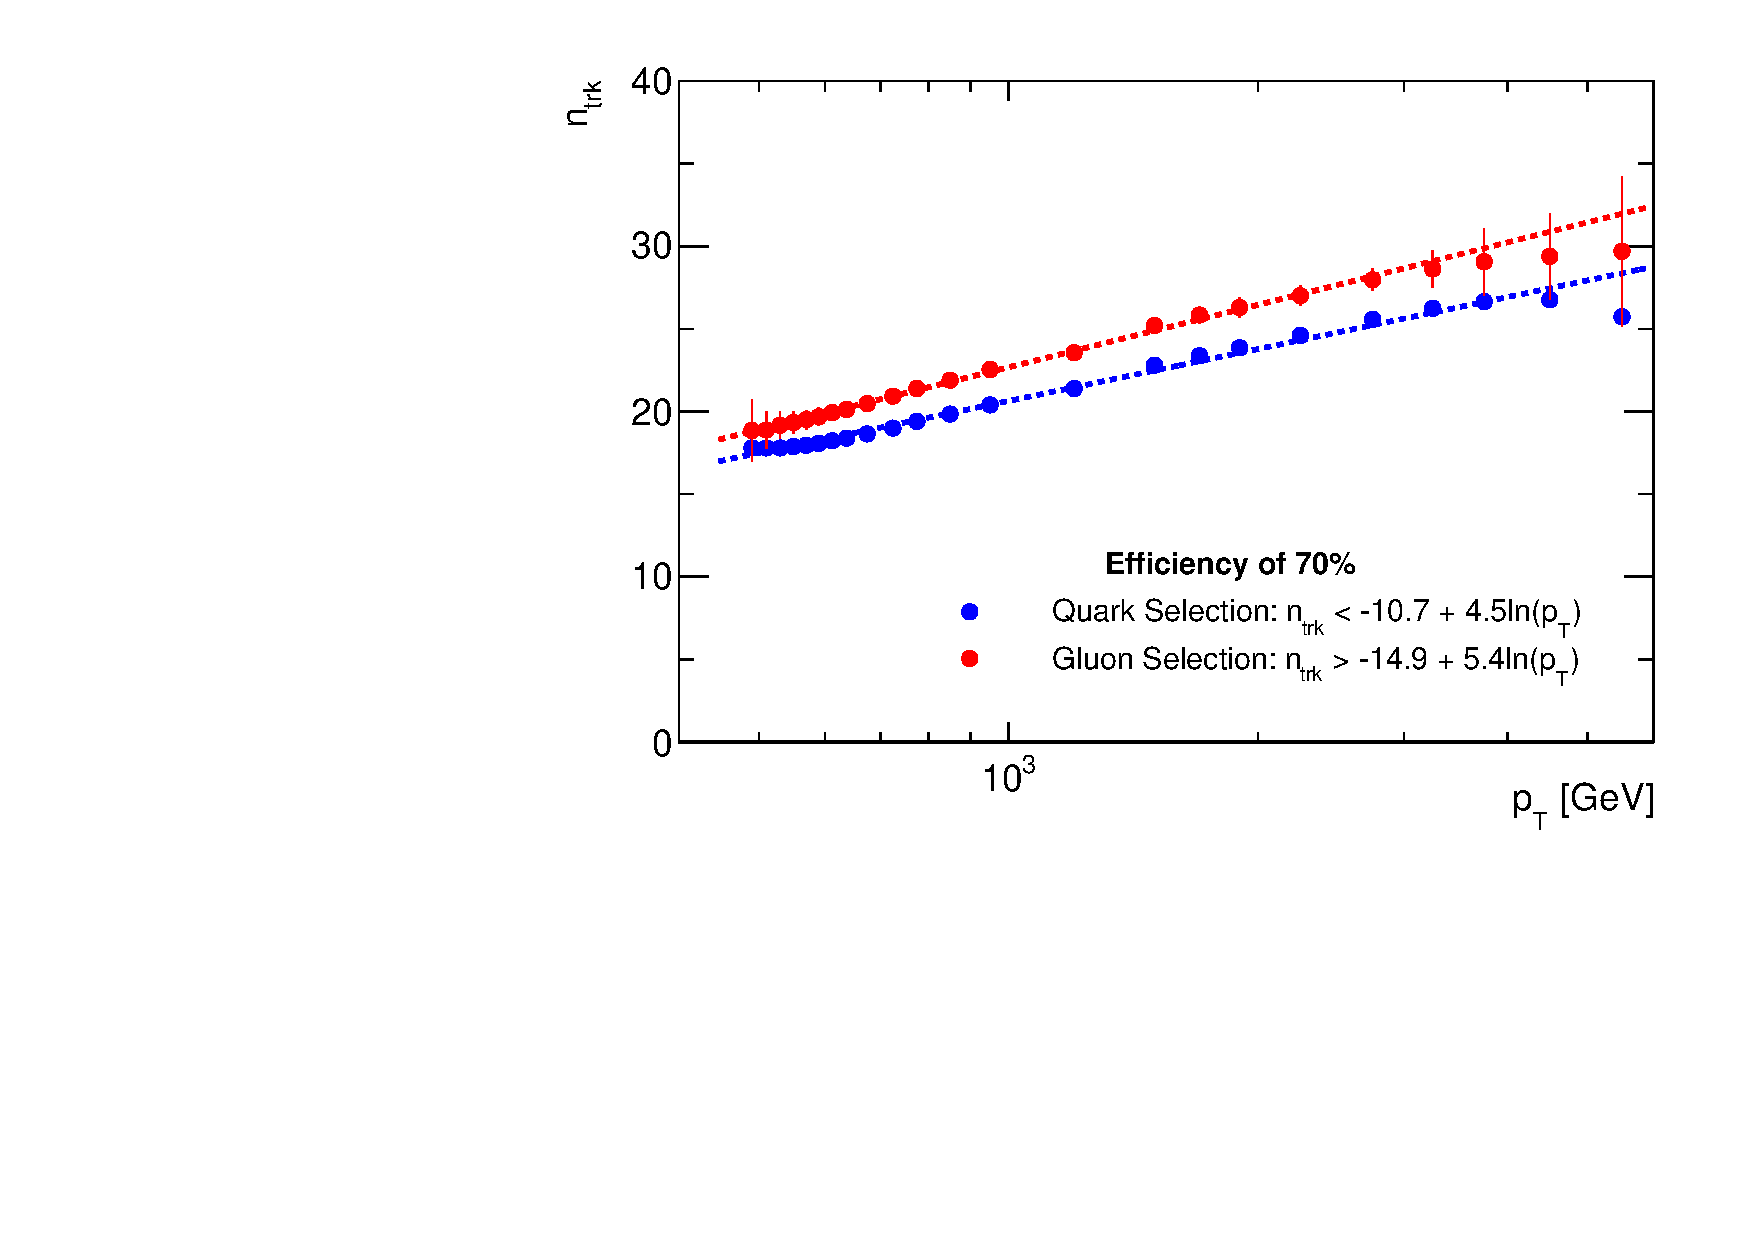
\includegraphics[width=0.45\textwidth]{fig/tagging_variation/quark_frac_selection_errors_6}}
	\subfloat[] {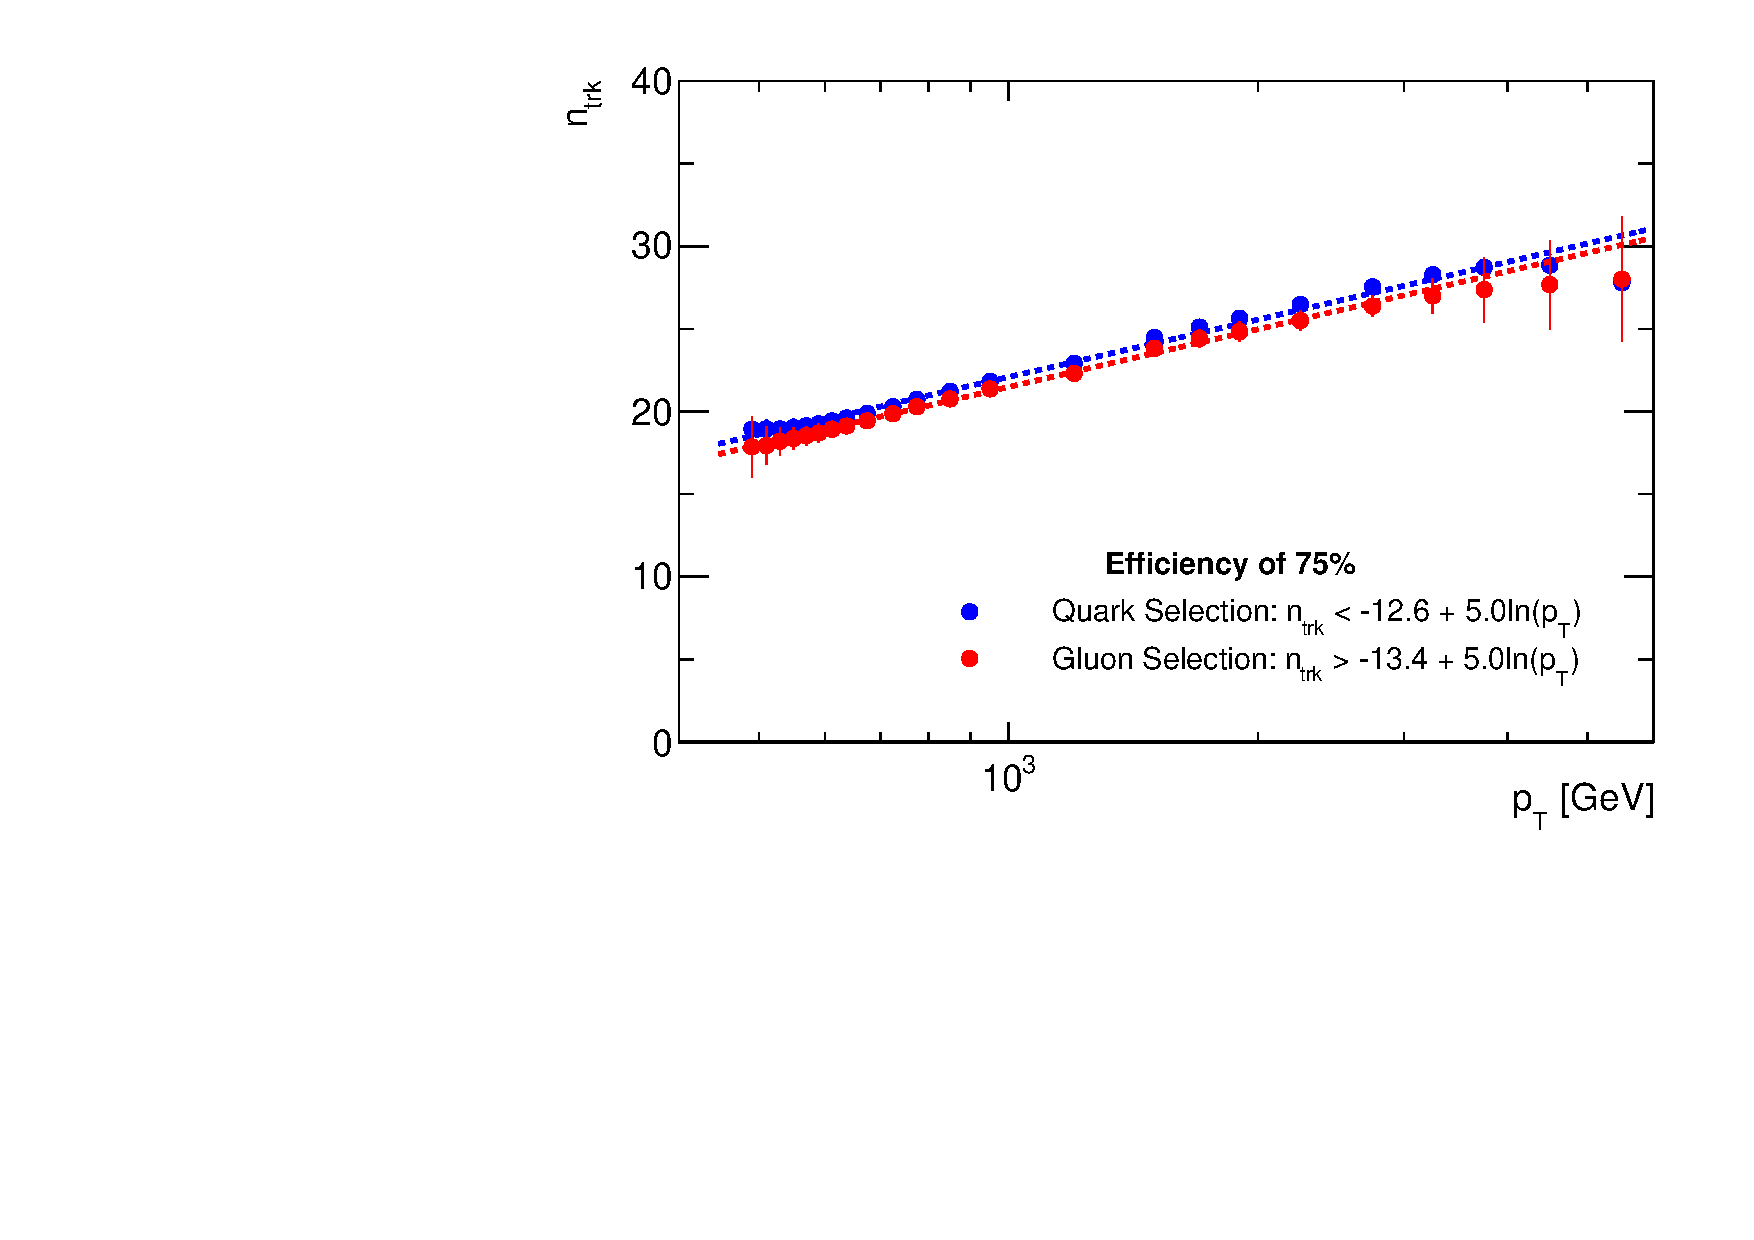
\includegraphics[width=0.45\textwidth]{fig/tagging_variation/quark_frac_selection_errors_5}}\\
	\subfloat[] {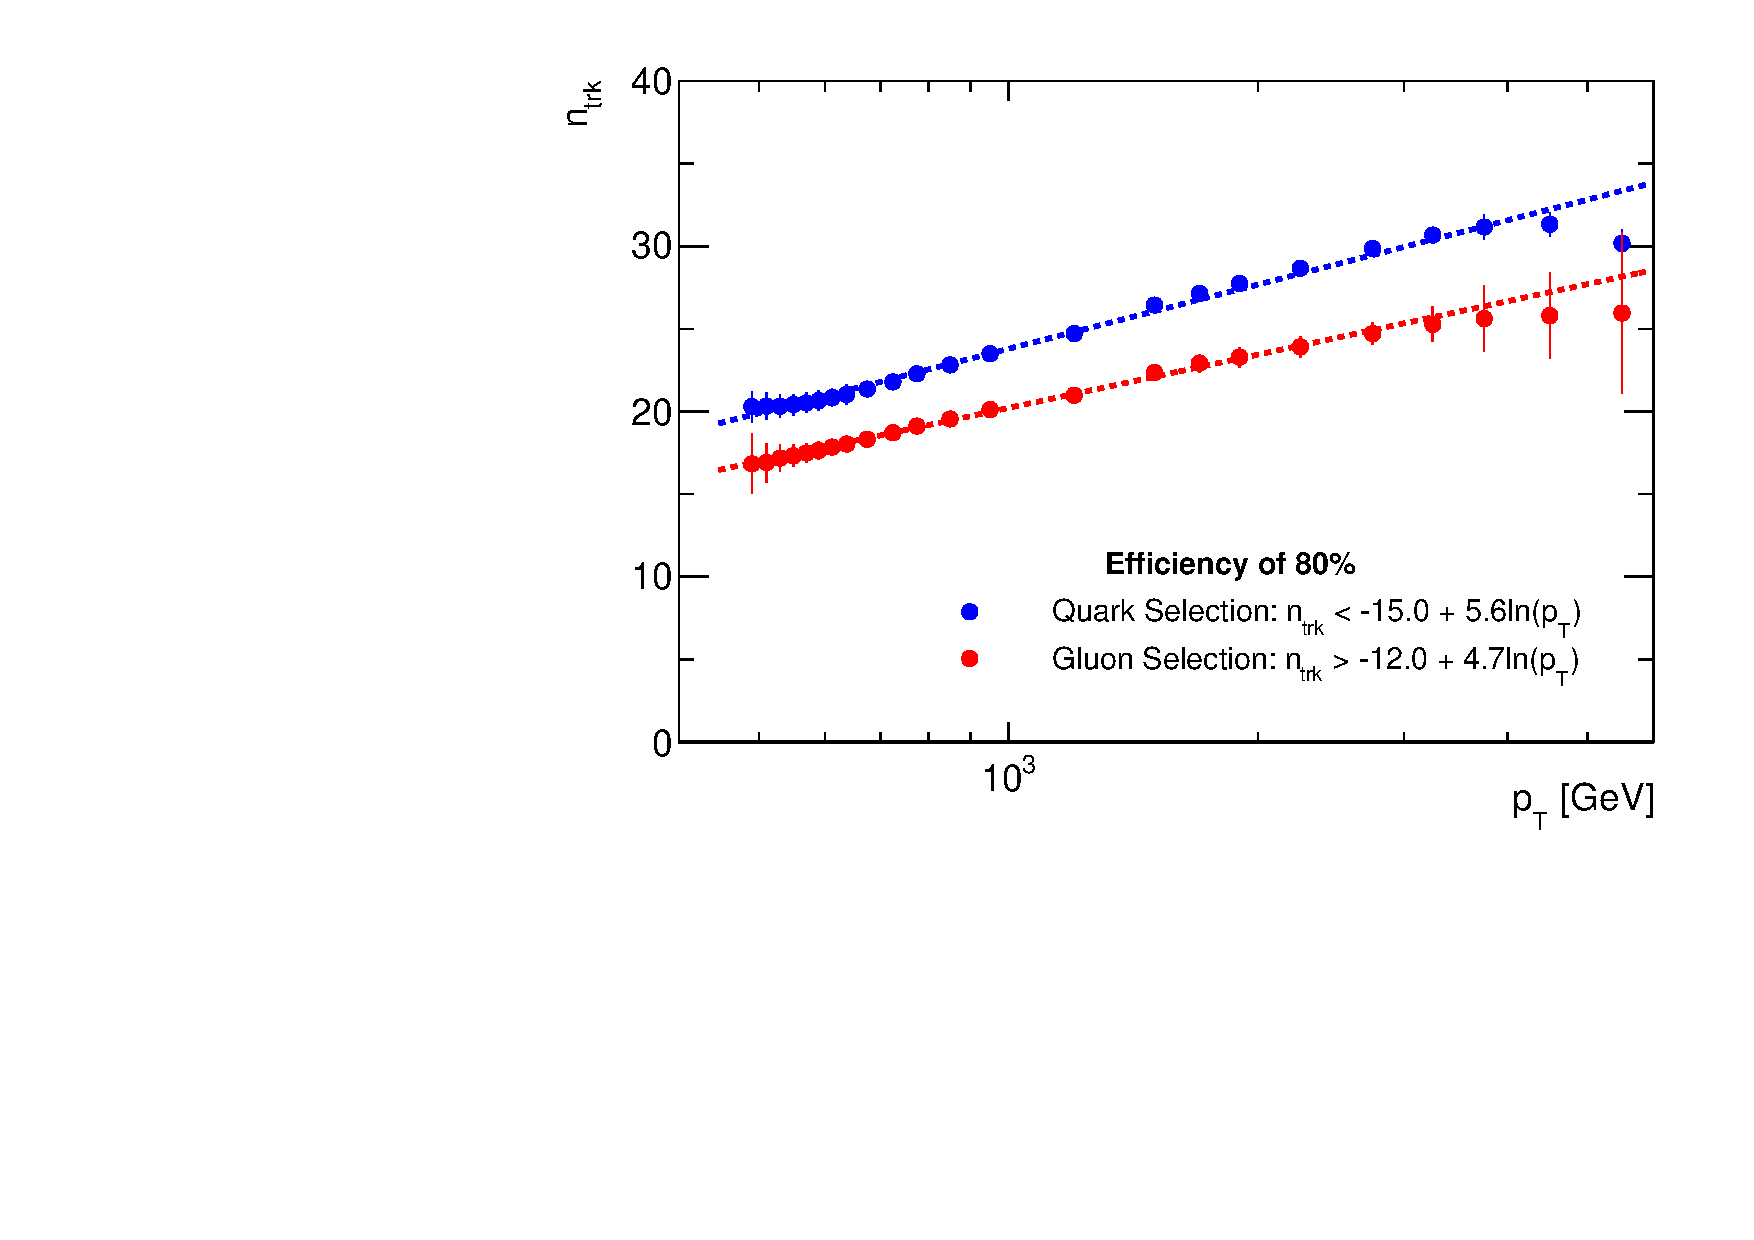
\includegraphics[width=0.45\textwidth]{fig/tagging_variation/quark_frac_selection_errors_4}}
	
	\caption{ The values of \ntrk\ for (a) 70\%,  (b) 75\%  and (c) 80\% quark (blue) and gluon (red) 
		selection efficiencies in each \pt\ bin along with the best fit to Equation~\ref{eq:nqg2}.
		\label{fig:qg_selection_curves_app}}
\end{figure}

\begin{figure}[p]
	\centering
	\subfloat[] {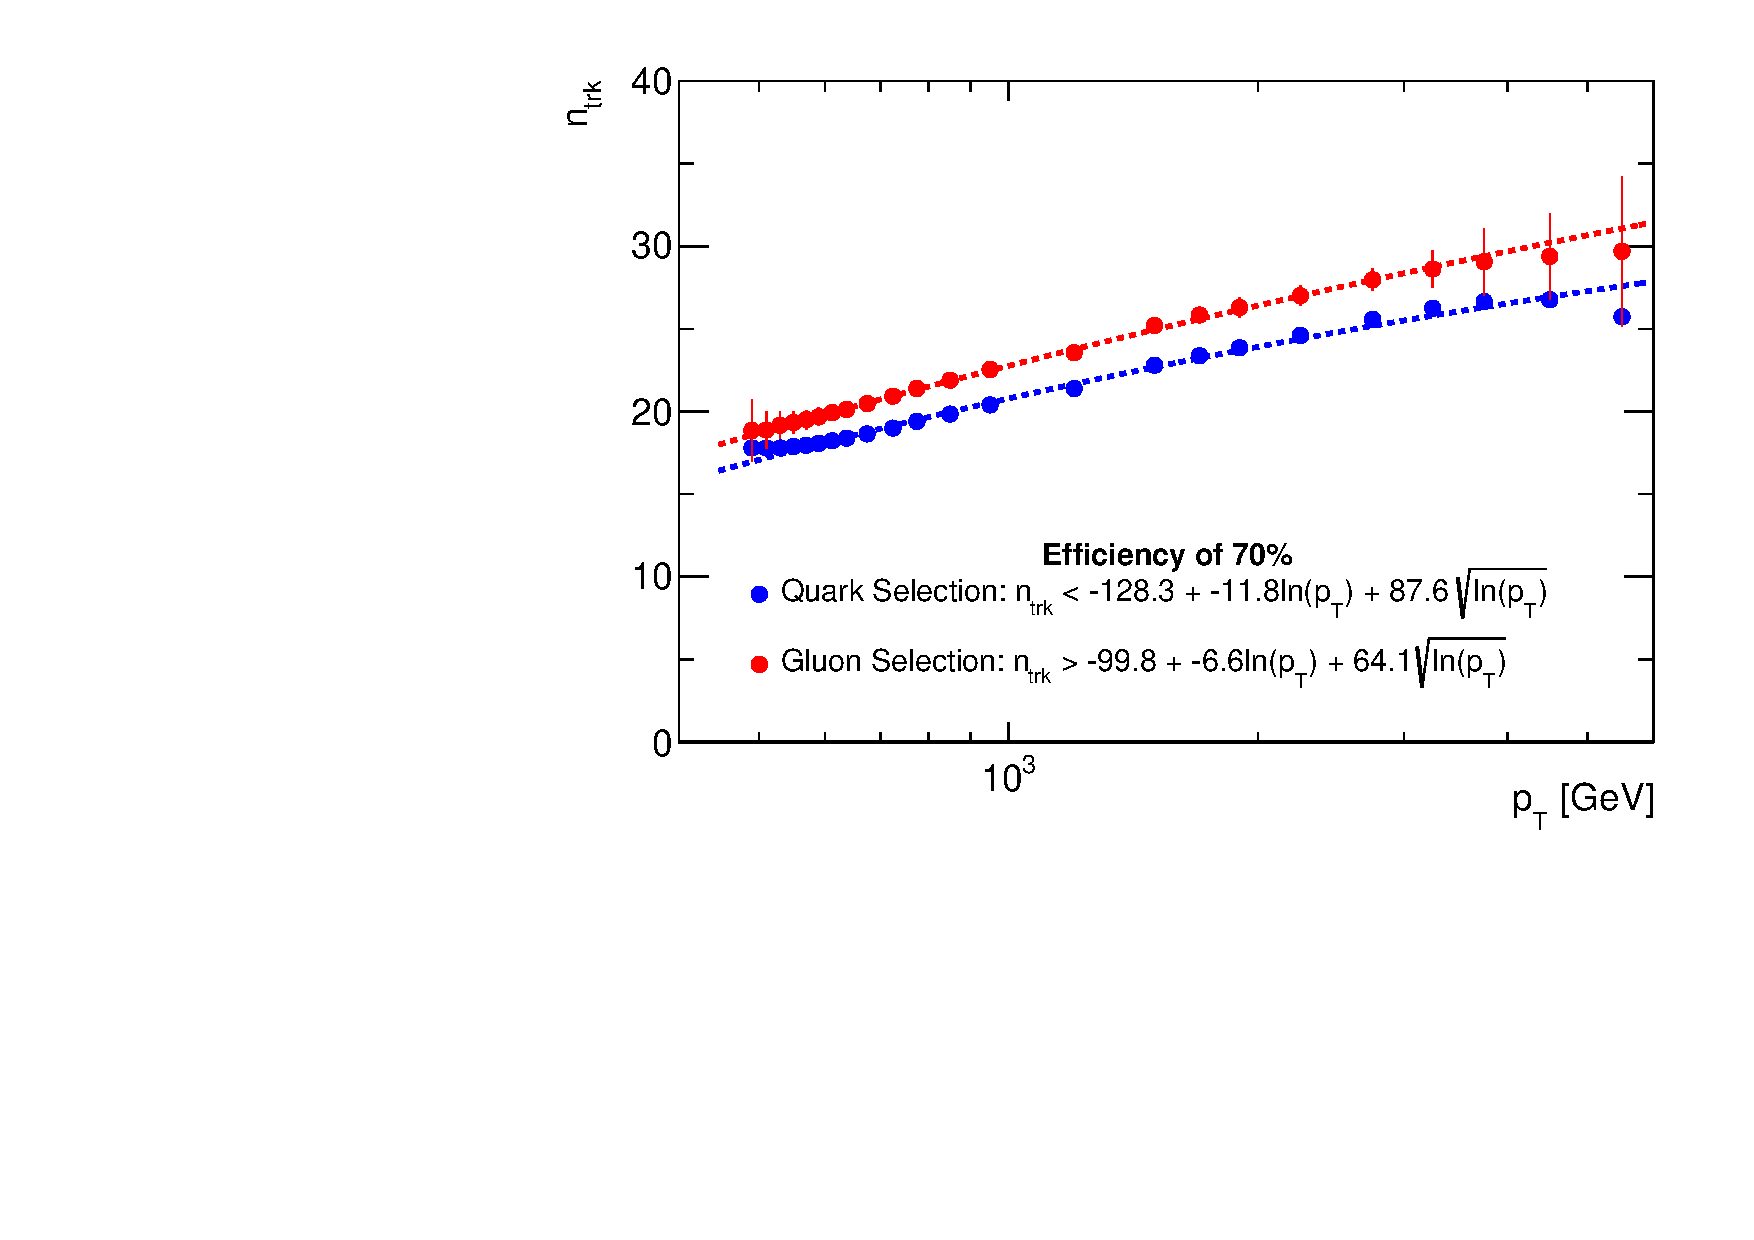
\includegraphics[width=0.45\textwidth]{fig/tagging_variation/quark_frac_newFit_selection_errors_6}}
	\subfloat[] {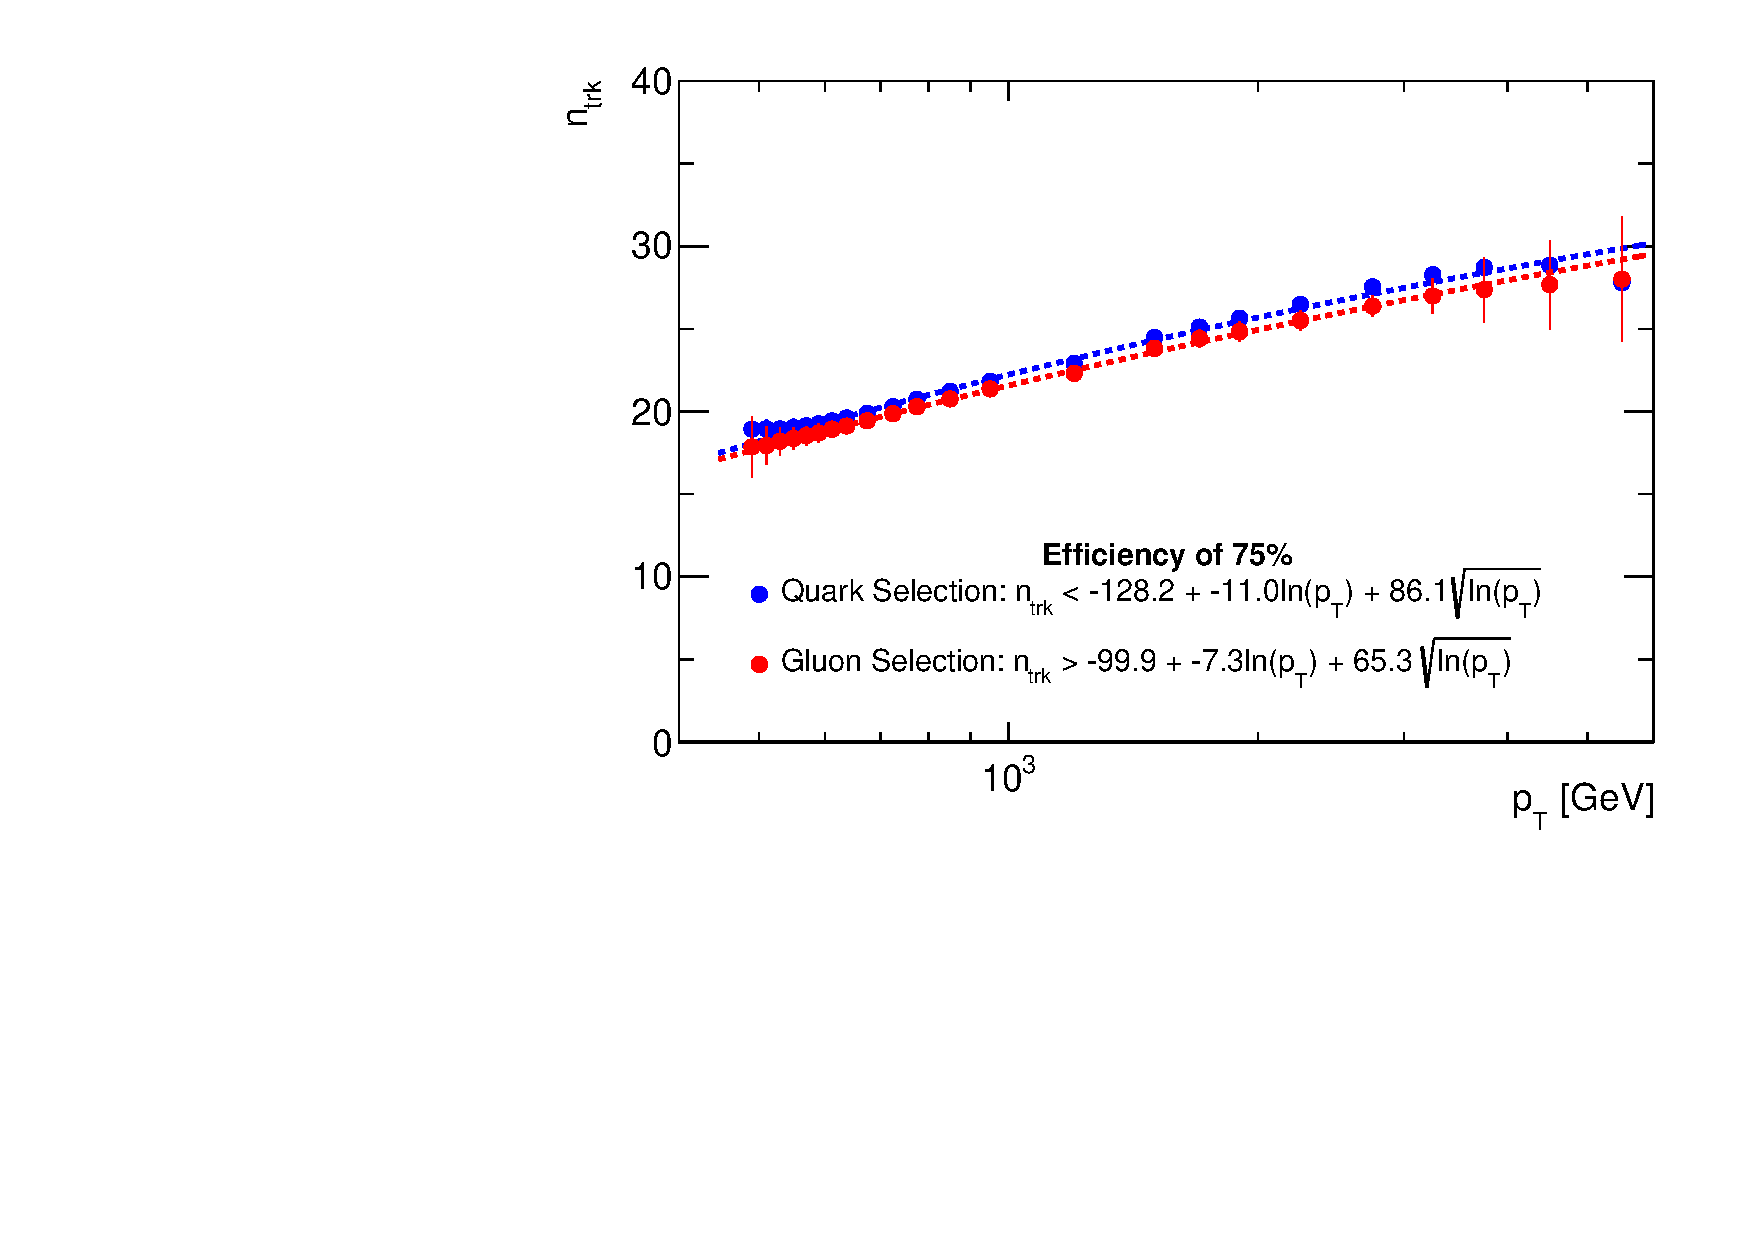
\includegraphics[width=0.45\textwidth]{fig/tagging_variation/quark_frac_newFit_selection_errors_5}}\\
	\subfloat[] {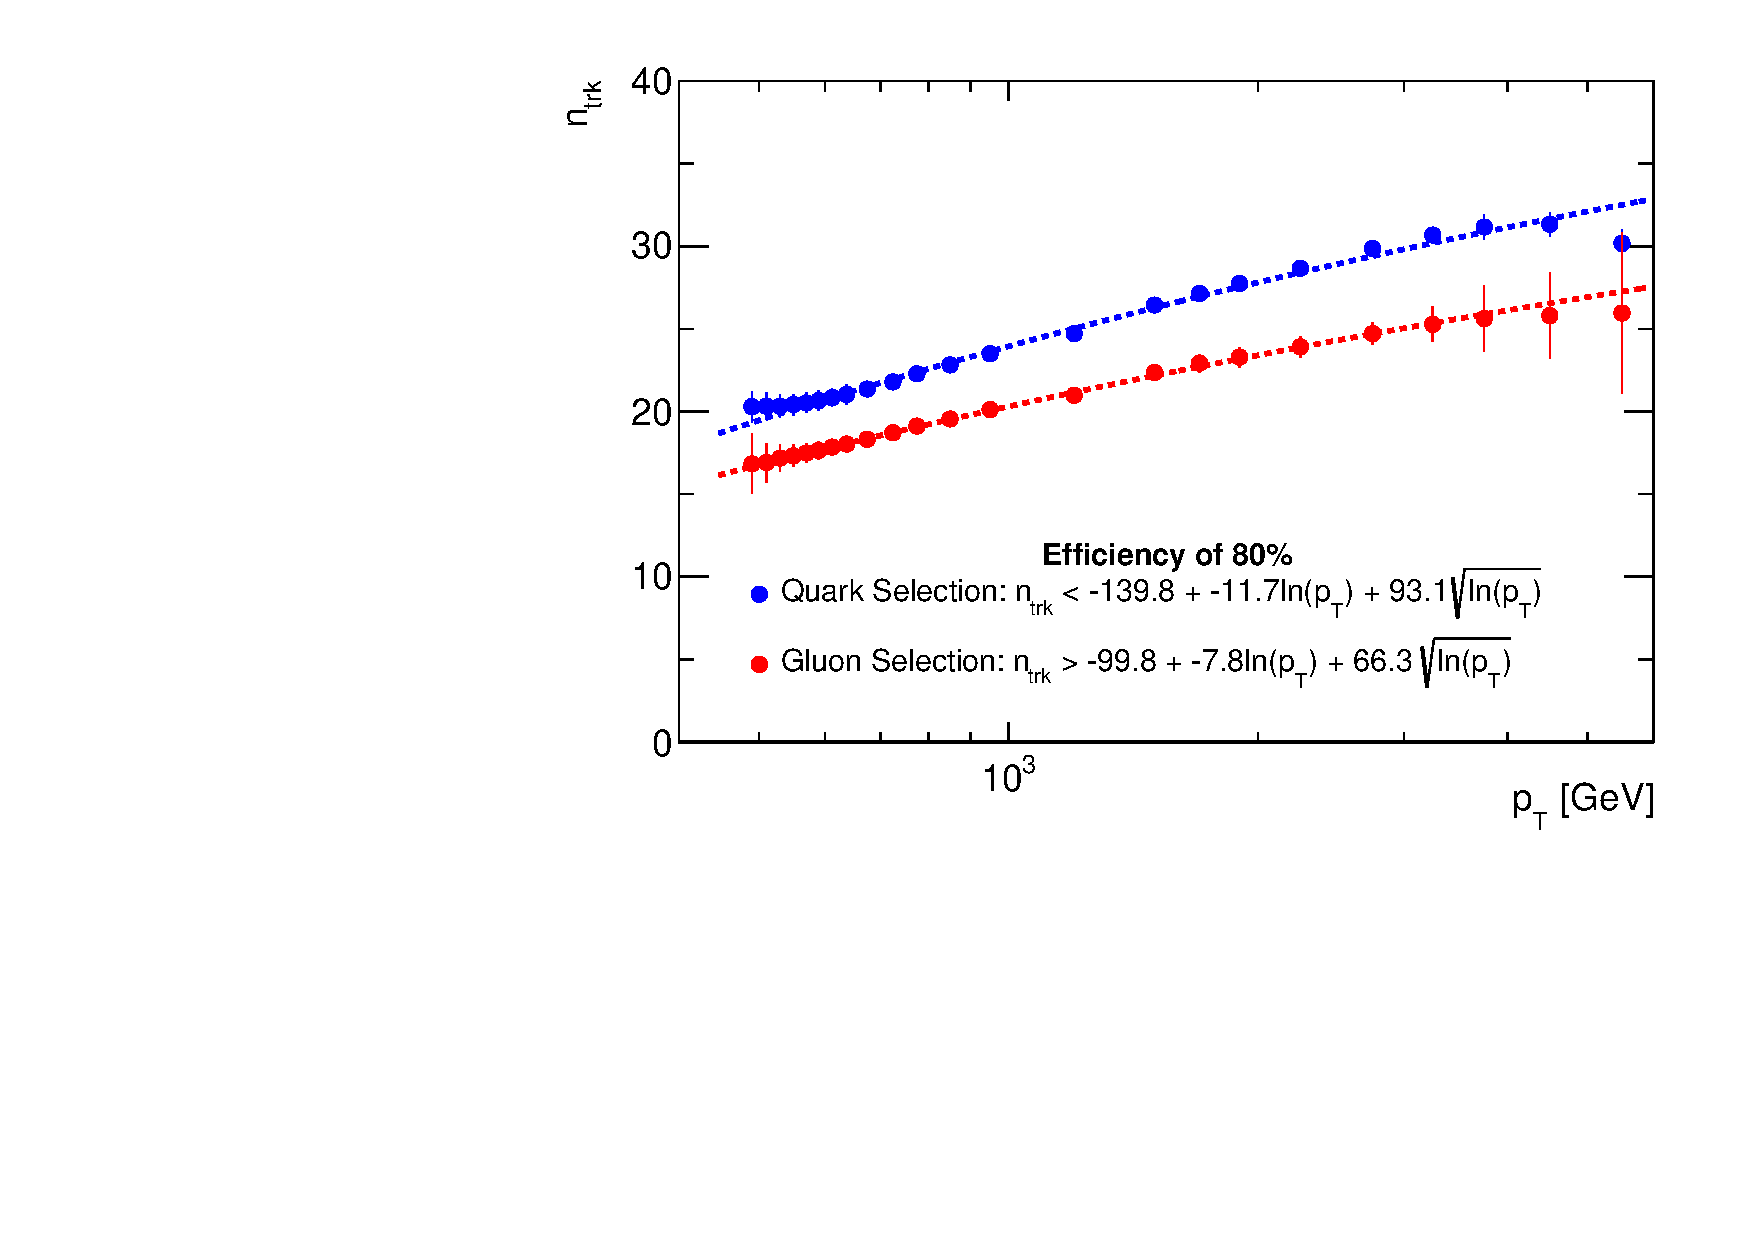
\includegraphics[width=0.45\textwidth]{fig/tagging_variation/quark_frac_newFit_selection_errors_4}}
	
	\caption{ The values of \ntrk\ for (a) 70\%,  (b) 75\%  and (c) 80\% quark (blue) and gluon (red) 
		selection efficiencies in each \pt~bin along with the best fit to Equation~\ref{eq:nqg3}.
		\label{fig:qg_selection_curves2}}
\end{figure}



\begin{table}[h]
	\centering 
	
	\begin{tabular}{SSSSS}
	\toprule
\multicolumn{1}{c}{Truth-$g$ selection efficiency}   & \multicolumn{1}{c}{Truth-$q$ selection efficiency} &  \multicolumn{1}{c}{$c$}  &  \multicolumn{1}{c}{$m$} &  \multicolumn{1}{c}{$n$}  \\
\midrule 
0.80 & 0.320 & -99.796 & -7.839 & 66.301 \\
0.75 & 0.274 & -99.949 & -7.271 & 65.347 \\
0.70 & 0.234 & -99.774 & -6.640 & 64.077 \\
\bottomrule
\end{tabular}
	\caption{ Values of constants $m$ and $c$ from Equation~\ref{eq:nqg3} such that $ \ntrk  \ge \ngluon $ 
	for truth quark jets for a range of efficiencies  from 70 to 80\%. 
	\label{table:truthGluonSelectionEfficiencies2}
}
\end{table}


\FloatBarrier


\paragraph{Signal Selection Efficiencies\\}

The \Hprime\ signal described in section~\ref{sec:hprime} is required to pass the selection criteria for a single jet gluon selection efficiency of 75\% given in Table~\ref{table:HprimeselctionEfficiency_app}. The selection efficiency for the \Hprime\ sample is expected to be 56.3\% ($0.75^2$ as both jets are required to be 75\%). In actual process, the ratio of \Hprime\ events that decay to two gluons ranges from 51.9\% for a 2 TeV signal to 57.4\% for a 7 TeV signal.

The effective fraction of \Hprime\ events decaying into two gluons is slightly below 100\%, due to factors like gluon splitting and other showering effects. This fraction varies from 91.3\% to 95.4\%. The discrepancy between the actual efficiency and the expected efficiency (56.3\% of the truth efficiency) is depicted in Figure~\ref{fig:HPrime_efficiency_difference}. The average difference across selection criteria is approximately 3.3\%.

Since there is minimal distinction between the two selection criteria, the simpler choice outlined in Equation~\ref{eq:nqg2} will be adopted.

\begin{table}[h]
	\centering 
	\begin{tabular}{SSSS}
	\toprule
\multicolumn{1}{c}{\Hprime\ Mass (GeV)}   & \multicolumn{3}{c}{Selection efficiency(\%)} \\
\multicolumn{1}{c}{} & \multicolumn{1}{c}{Equation~\ref{eq:nqg2}} & \multicolumn{1}{c}{Equation.~\ref{eq:nqg3} ($\sqrt{}$ term)} 
& \multicolumn{1}{c}{Truth} \\
\midrule 
2000	&	51.9 & 51.8& 91.3 \\
2500	&	53.2 & 53.0& 91.7 \\
3000 	&	54.9 & 54.6& 92.3 \\
3500	&	55.3 & 55.1& 93.4 \\
4000	&	56.4 & 56.2& 93.4 \\
4500	&	56.7 & 56.7& 94.1 \\
5000	&	56.2 & 56.4& 94.3 \\
5500	&	57.2 & 57.5& 94.9 \\
6000	&	57.4 & 57.8& 95.1 \\
6500	&	57.4 & 58.3& 95.5 \\
7000	&	57.4 & 58.1& 95.4 \\\bottomrule
\end{tabular}
	\caption{ The signal selection efficiency for a fully simulated \Hprime\ decaying to two gluons with requiring two jets to 
	pass the 75\% single jet criteria given in Equation~\ref{eq:nqg2} with constants from 
	Table~\ref{table:truthGluonSelectionEfficiencies_app} and the criteria given in Equation~\ref{eq:nqg3} with constants from 
	Table~\ref{table:truthGluonSelectionEfficiencies2}.  
	The expected double tagged gluon efficiency is 56.3\%. 
	\label{table:HprimeselctionEfficiency_app}
}
\end{table}


\begin{figure}[p]
 \centering
 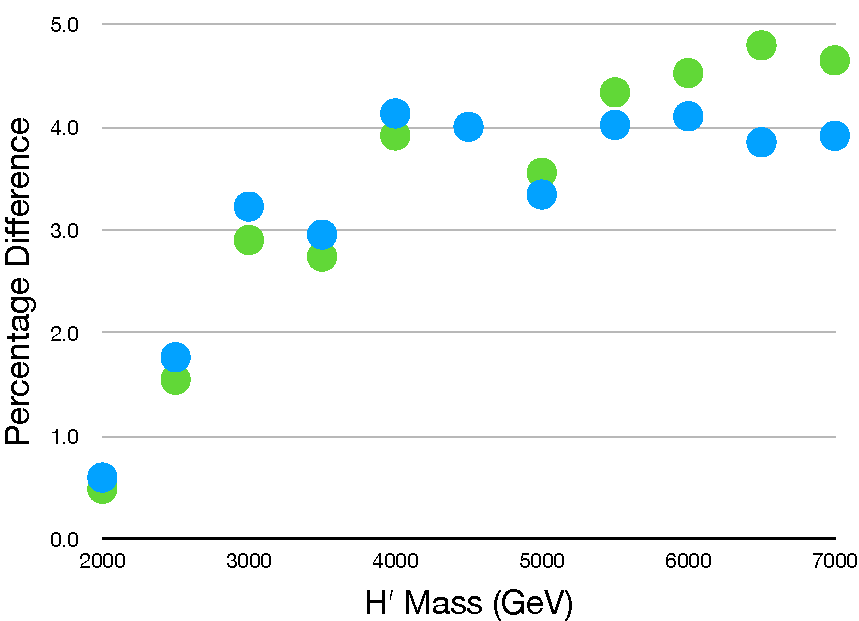
\includegraphics[width=0.60\textwidth]{fig/tagging_variation/HPrime_Efficiency_Difference}
\caption{ The difference between the expected signal selection efficiency of 56.3\%
for a single jet selection efficiency of 75\% for \Hprime\ using Equation~\ref{eq:nqg2} (Blue) and
Equation~\ref{eq:nqg3} (Green)}
 \label{fig:HPrime_efficiency_difference}}
\end{figure}




%The constants $m$ and $c$ are found by finding the value of \ntrk\ 
%that corresponds to a given efficiency for truth quark and gluon jets in 
%\pT\ bins and fitting the results. For each \pT\ bin the number of tracks 
%closest to the chosen selection efficiency is found. Since this is an integer 
%number of tracks and does and does not correspond exactly to the selection efficiency 
%a correction is applied by estimating the fractional number of tracks that corresponds 
%to the selection  efficiency  by carrying out a linear interpolation between the efficiencies 
%for the selected bin and its nearest neighbour. The uncertainty on this value is then estimated using 
%binomial uncertainties. 



%The constants $m_{\mathrm{q(g)}}$ and $c_{\mathrm{q(g)}}$ are found by finding the value of \ntrk\ 
%that corresponds to a given efficiency for truth quark and gluon jets in 
%\pT\ bins and fitting the results to Eq.~\ref{eq:nqg2}.  The jet \pT\ bin edges are chosen to be 
%400, 500, 650, 800, 1000, 1200, 1500, 2000, 3000, 6000\,\GeV. An example of the \ntrk cumulative 
%distribution for truth quark and gluon jets satisfying $800 < \pT < 1000\,\GeV$ is shown in
%Fig.~\ref{fig:ntrk_cumulative}.
%
%
%
%%The jet \pT\ bin edges are chosen to be 
%%480, 500, 520, 540, 560, 580, 600, 625, 650, 700, 750, 800, 900, 1000, 1400, 
%%1600, 1800, 2000, 2500, 3000, 3500, 4000, 5000, 6000\,\GeV. An example of the \ntrk cumulative 
%%distribution for truth quark and gluon jets satisfying $800 < \pT < 900\,\GeV$ is shown in
%%Fig.~\ref{fig:ntrk_cumulative}.
%
%
%%\begin{figure}[htb]
%% \centering
%%\includegraphics[width=0.75\textwidth]{figures/tagging/Cumulative_ntrk_distribution_12_800_900GeV.pdf}
%%\caption{The cumulative distribution of \ntrk\ for truth quark (blue) and gluon (red) initiated jets 
%%satisfying $800 < \pT < 900\,\GeV$.  \label{fig:ntrk_cumulative}}
%%\end{figure}
%
%\begin{figure}[htb]
% \centering
%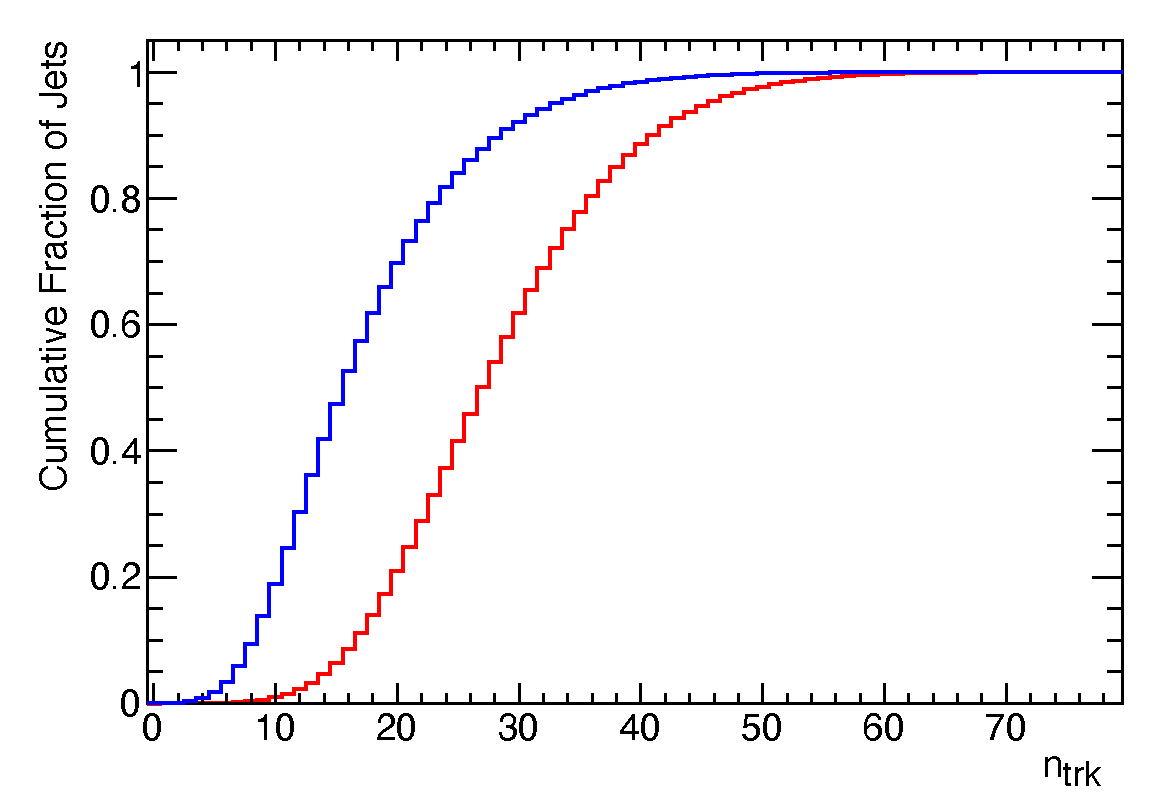
\includegraphics[width=0.75\textwidth]{figures/tagging/Cumulative_ntrk_distribution_4_800_1000GeV.pdf}
%\caption{The cumulative distribution of \ntrk\ for truth quark (blue) and gluon (red) initiated jets 
%satisfying $800 < \pT < 1000\,\GeV$.  \label{fig:ntrk_cumulative}}
%\end{figure}
%
%
%The constants for Eq.~\ref{eq:nqg2} are found for quark and gluon selection efficiencies from 
%65\% to 95\% in 5\% steps. The plot of the value of \ntrk\ that satisfies the selection efficiencies 
%of 70 and 80\% are shown in Fig.~\ref{fig:qg_selection_curves} along with the best fit using Eq.~\ref{eq:nqg2}.
%The values of the constants for both quark and gluon selections are summarised in 
%Tables~\ref{table:truthQuarkSelectionEfficiencies} and \ref{table:truthGluonSelectionEfficiencies}.
%
%\begin{figure}[htb]
% \centering
%  \subfigure[] {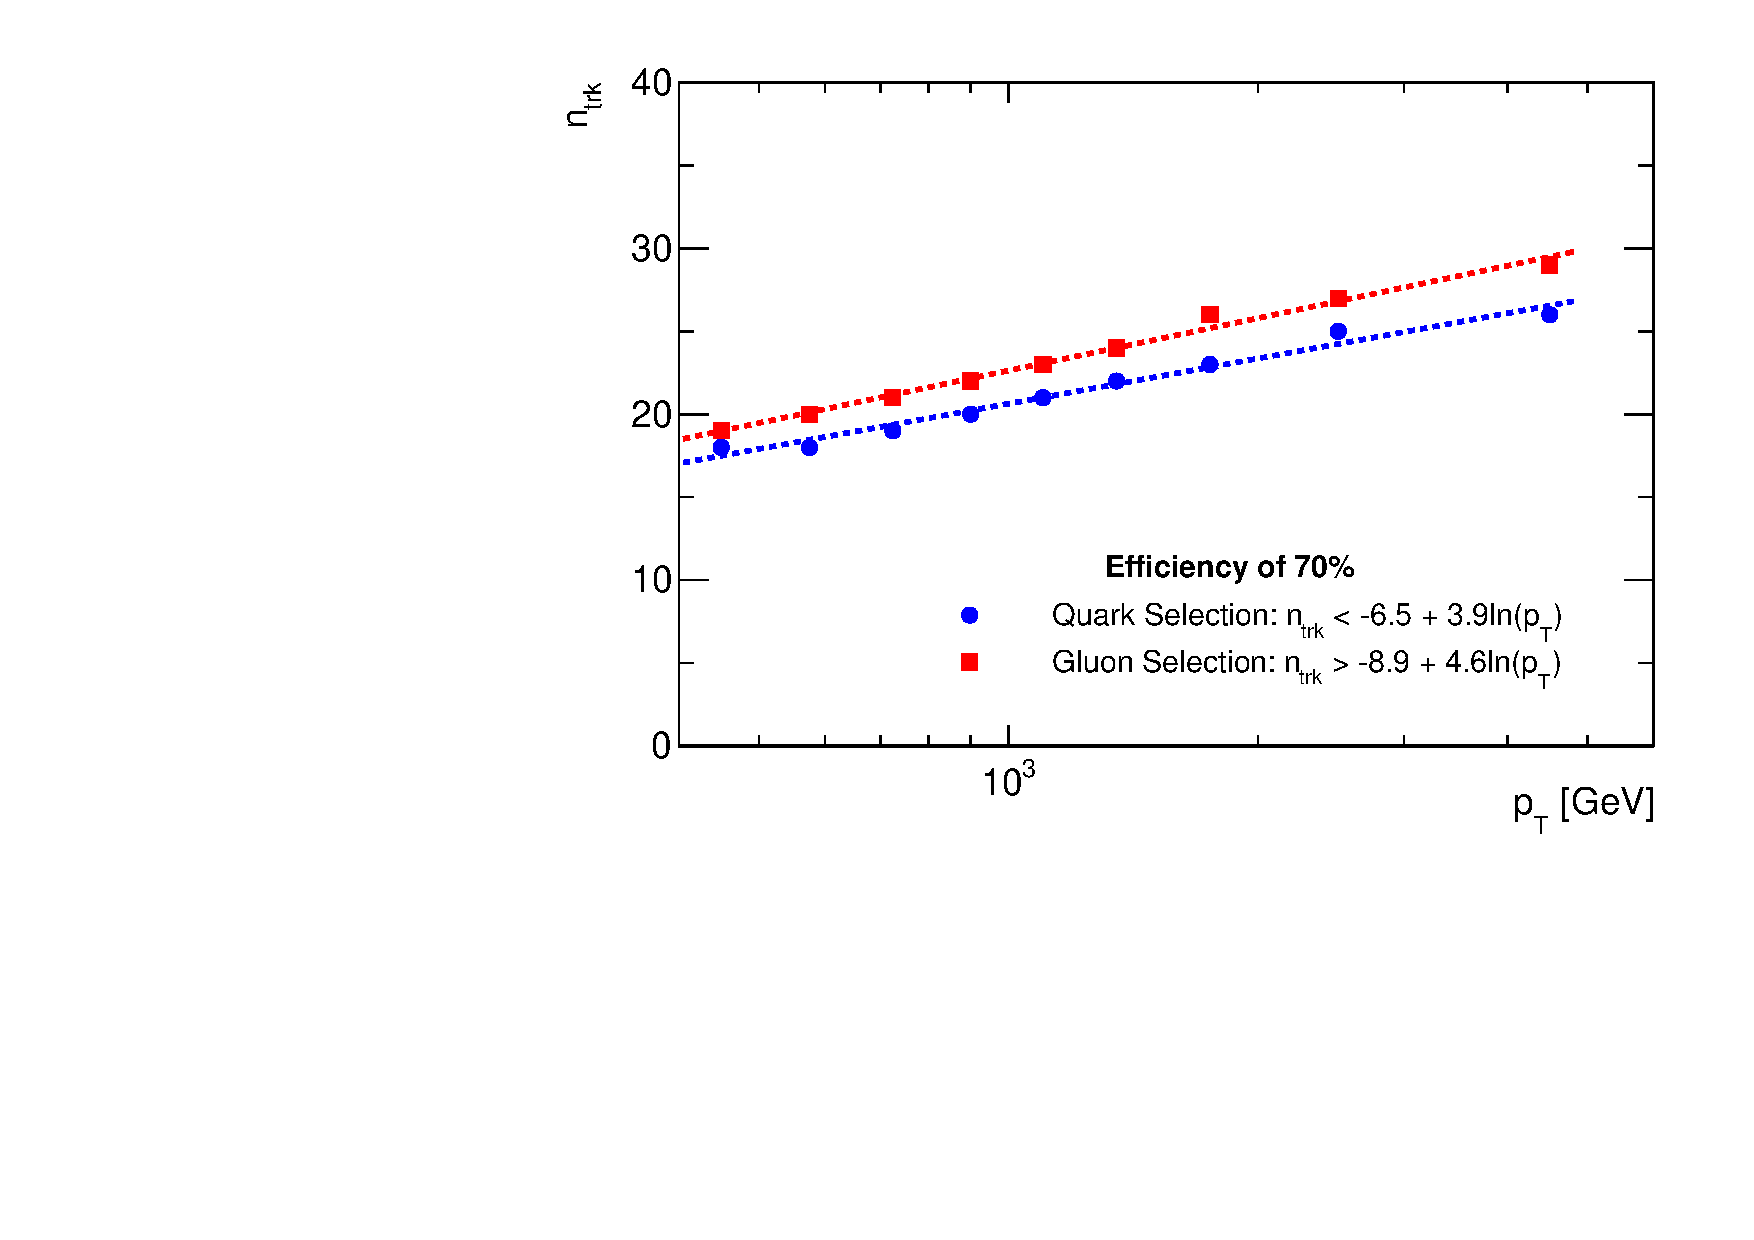
\includegraphics[width=0.495\textwidth]{figures/tagging/quark_selection_6}}
%  \subfigure[] {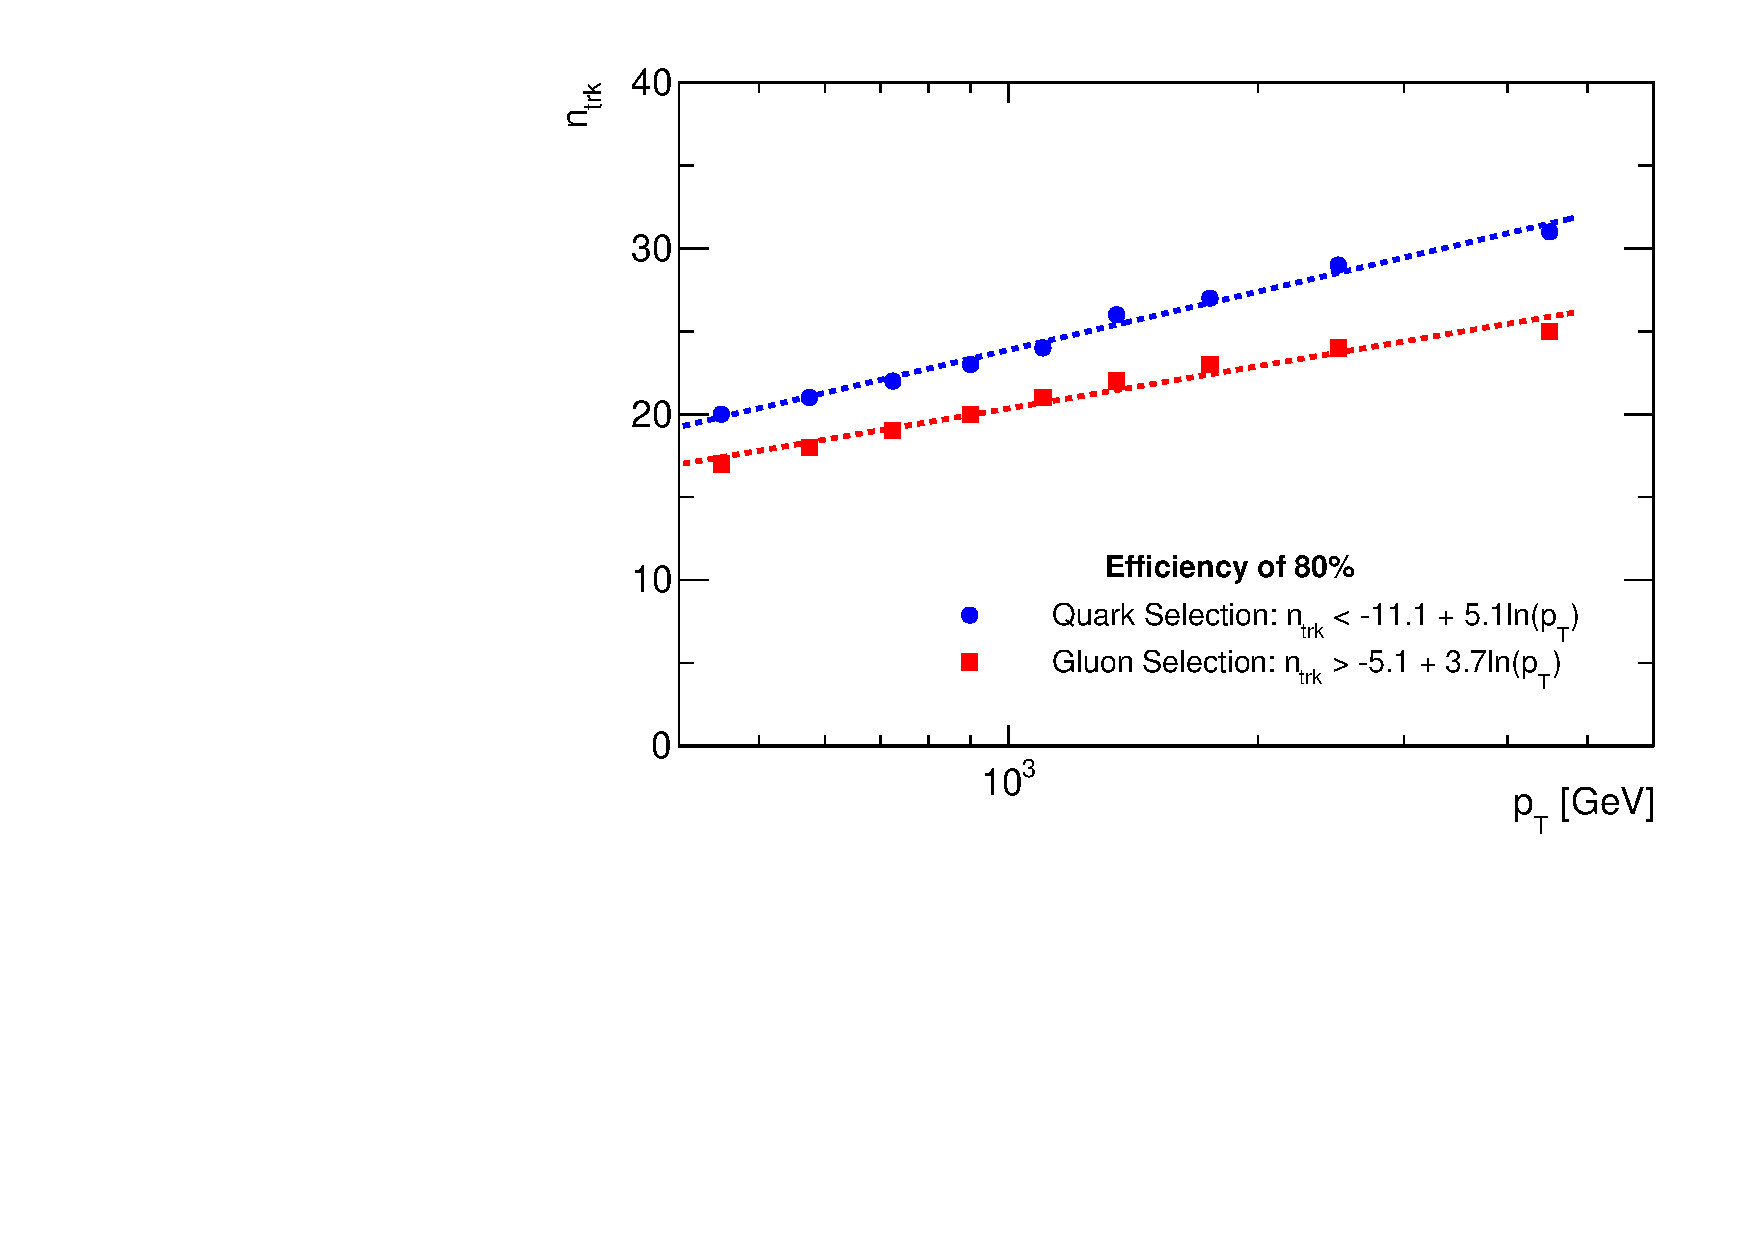
\includegraphics[width=0.495\textwidth]{figures/tagging/quark_selection_4}}
%
%\caption{ The values of \ntrk\ for (a) 70\% and (b) 80\% quark (blue) and gluon (red) 
%selection efficiencies in each \pT\ bin along with the best fit to Eq.~\ref{eq:nqg2}.
% \label{fig:qg_selection_curves}}
%\end{figure}
%
%
%\begin{table}[h]
%	\centering 
%		\caption{ Values of constants $m$ and $c$ from Eq.~\ref{eq:nqg2} such that $ \ntrk  \le \nq $ 
%		for truth quark jets for a range of efficiencies  from 65 to 95\%. 
%		\label{table:truthQuarkSelectionEfficiencies}
%		}
%	\begin{tabular}{SSSS}
%	\toprule
%\multicolumn{1}{c}{Truth-$q$ selection efficiency}   & \multicolumn{1}{c}{Truth-$g$ selection efficiency} &  \multicolumn{1}{c}{$c_{\mathrm{q}}$}  &  \multicolumn{1}{c}{$m_{\mathrm{q}}$} \\
%\midrule 
%0.95 & 0.73 & -20.0 & 7.7 \\
%0.90 & 0.57 & -15.9 & 6.5 \\
%0.85 & 0.45 & -13.1 & 5.6 \\
%0.80 & 0.36 & -11.1 & 5.1 \\
%0.75 & 0.28 & -9.1  & 4.5 \\
%0.70 & 0.22 & -6.5  & 3.9 \\
%0.65 & 0.18 & -4.4  & 3.5 \\
%\bottomrule
%\end{tabular}
%\end{table}
%
%\begin{table}[h]
%	\centering 
%		\caption{ Values of constants $m$ and $c$ from Eq.~\ref{eq:nqg2} such that $ \ntrk  \ge \ngluon $ 
%		for truth gluon jets for a range of efficiencies  from 65 to 95\%. 
%		\label{table:truthGluonSelectionEfficiencies}
%		}
%	\begin{tabular}{SSSS}
%	\toprule
%\multicolumn{1}{c}{Truth-$g$ selection efficiency}   & \multicolumn{1}{c}{Truth-$q$ selection efficiency} &  \multicolumn{1}{c}{$c_{\mathrm{g}}$}  &  \multicolumn{1}{c}{$m_{\mathrm{g}}$} \\
%\midrule 
%0.95 & 0.59 & -3.9 & 2.7 \\
%0.90 & 0.46 & -4.3 & 3.1 \\
%0.85 & 0.39 & -5.4 & 3.5 \\
%0.80 & 0.31 & -5.1 & 3.7 \\
%0.75 & 0.27 & -7.3 & 4.2 \\
%0.70 & 0.23 & -8.9 & 4.6 \\
%0.65 & 0.20 & -8.0 & 4.6\\
%\bottomrule
%\end{tabular}
%\end{table}
%
%
%\subsubsection{Signal Selection Efficiencies}
%
%
%The selection criteria for a single jet gluon selection efficiency of 75\% is applied to the \Hprime\ 
%sample described in in section~\ref{sec:hprime} are given in Table~\ref{table:HprimeselctionEfficiency}. 
%If the selection works perfectly the expected selection efficiency for the \Hprime\ sample would be 56.3\% ($0.75^2$). 
%The actual selection efficiencies range between 51.9\% for a 2\,\TeV\ signal to 57.4\% for a 7\,\TeV\ signal. 
%
%The actual fraction of \Hprime\ events that decay to two gluons is less than 100\% due to gluon splitting and other showering 
%effects and ranges from 91.3 to 95.4\%. The variation between the expected efficiency (56.3\% of the truth efficiency) 
%is plotted in Fig.~\ref{fig:HPrime_efficiency_difference}. The average difference for is approximately 3.3\% for both selection criteria.
%
%%There is negligible difference between the two selection criteria so the simpler choice as given in Eq.~\ref{eq:nqg2} will be used.
%
%
%
%\begin{table}[h]
%	\centering 
%		\caption{ The signal selection efficiency for a fully simulated \Hprime\ decaying to two gluons with requiring two jets to 
%		pass the 75\% single jet criteria given in Eq.~\ref{eq:nqg2} with constants from 
%		Table~\ref{table:truthGluonSelectionEfficiencies} and the criteria given in Eq.~\ref{eq:nqg3} with constants from 
%		Table~\ref{table:truthGluonSelectionEfficiencies2}.  
%		The expected double tagged gluon efficiency is 56.3\%. 
%		\label{table:HprimeselctionEfficiency}
%		}
%	\begin{tabular}{SSS}
%	\toprule
%\multicolumn{1}{c}{\Hprime\ Mass (\GeV)}   & \multicolumn{2}{c}{Selection efficiency(\%)} \\
%\multicolumn{1}{c}{} & \multicolumn{1}{c}{Eq.~\ref{eq:nqg2}} &  \multicolumn{1}{c}{Truth} \\
%\midrule 
%2000	&	51.9 & 91.3 \\
%2500	&	53.2 & 91.7 \\
%3000 	&	54.9 & 92.3 \\
%3500	&	55.3 & 93.4 \\
%4000	&	56.4 & 93.4 \\
%4500	&	56.7 & 94.1 \\
%5000	&	56.2 & 94.3 \\
%5500	&	57.2 & 94.9 \\
%6000	&	57.4 & 95.1 \\
%6500	&	57.4 & 95.5 \\
%7000	&	57.4 & 95.4 \\\bottomrule
%\end{tabular}
%\end{table}
%
%
%\clearpage
%

\clearpage

\subsection{Signal optimisation}
\label{sec:Optimisation} % uncomment if label used. 
\subsubsection{\ystar\ Cut Optimisation}
\label{section:ystarCutOptimization}

%\todo[inline]{ Clean up formulae. }

In QCD, $t$-channel in 2-to-2 scattering is the dominant process. Thus the dijet production from the QCD is proportional to $\displaystyle{(1-\cos\theta^{*})^{-2}}$. However the distribution of $\cos\theta^{*}$ is supposed to be flat for $H^\prime$ signal, which means the \ystar\ of $H^\prime$ signal will peak at 0 while that of QCD background will minimize at 0.


The significance is defined as: 
\begin{equation}
\label{eq:signifcanceYstar} % uncomment if label used.
S  = \sqrt{\sum_{i}{2\left[ \left(S_{i}+B_{i} \right)\cdot \ln \left(1+\frac{S_{i}}{B_{i}}\right)-S_{i}\right]}}
\end{equation}
where $S_i$ ($B_i$) is the number of signal (background) events in bin $i$. 
The calculation of such significance only include the bins where signal samples have 95\% of the area under the distribution, not include the entire \mjj\ distribution.

For some signal samples where $S_i$ is small ($S_i << 10^{-5}$) thus the logarithm functions do not have
enough precision in equation \ref{eq:signifcanceYstar}. An approximation is introduced as follows:
\begin{equation}
%\label{eq:significanceYstarApprox}
S = \sqrt{\sum_{i}{2\sum_{n=1}^{6}{\frac{(-S_i)^{n+1}}{n \left(n+1 \right) B_i^n}}}}
\end{equation}
which is accurate up to 10 decimal places around $\frac{S_i}{B_i} = 10^{-5}$ and even more precise for smaller $\frac{S_i}{B_i}$.

%The significance of $H^\prime$ signal as a function 
%of the value of the \ystar\ is shown in Figure.~\ref{fig: hprime significance as a function of y* cut}. The peaks of significance in all tagging categories are around 0.6, therefore an optimal $y^{*}$ cut for the $H'$ search is set to
%$|\ystar| < 0.6$. The exact values of \ystar\ cut that correspond to the peak significance value for the $H^\prime$ signal at each mass point are shown in Table~\ref{tab:ystarhprime} with the ranges in \ystar\ cut around the peak that gives a significance $\geq$ 0.99.
%
%\begin{figure}[!htb]
%        \centering
%        \subfloat[Inclusive]{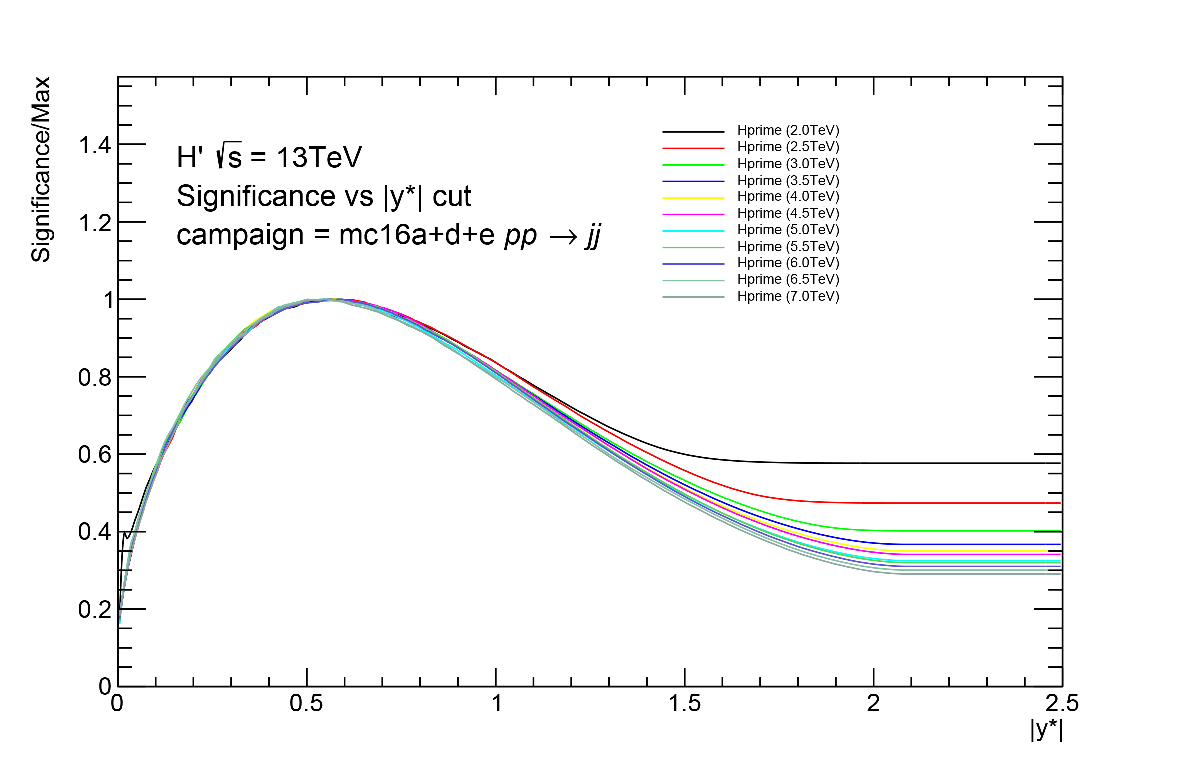
\includegraphics[width=0.45\columnwidth]{fig/yStarOptimization/New_Plots/Significance_Hprime_mc16a+d+e_jj.pdf}}
%        \subfloat[$\geq$1 g-tag]{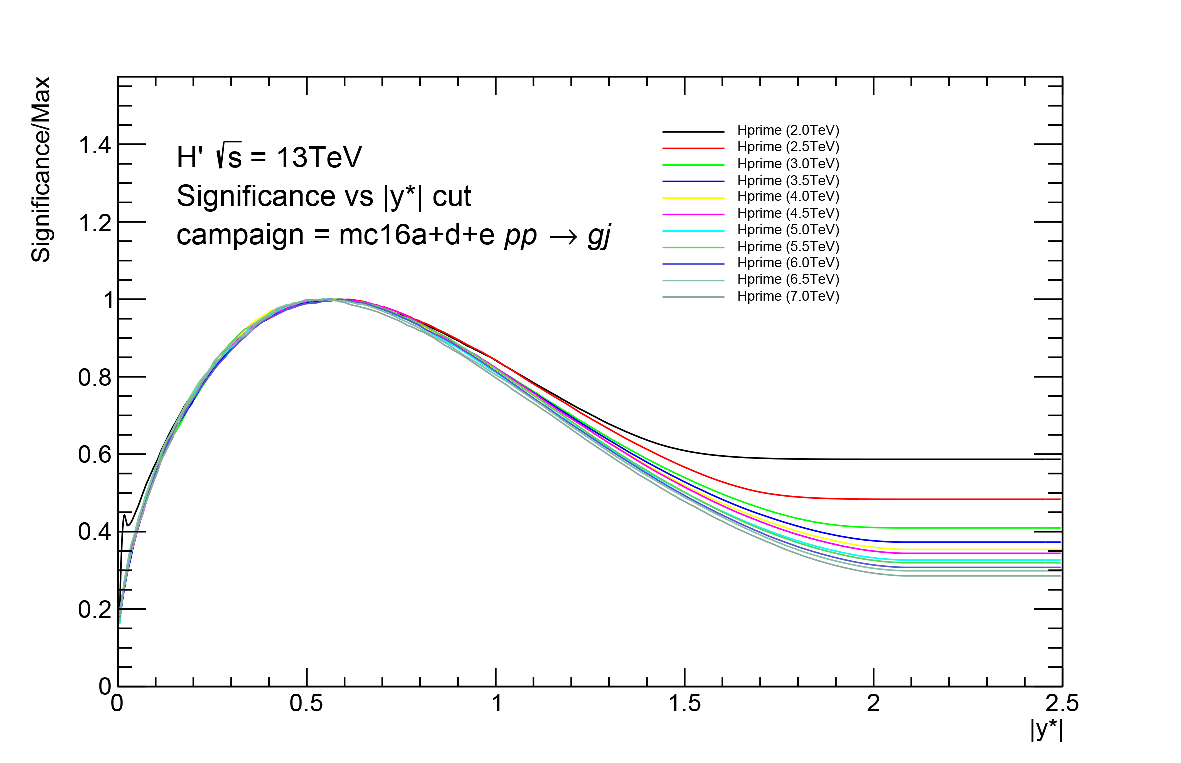
\includegraphics[width=0.45\columnwidth]{fig/yStarOptimization/New_Plots/Significance_Hprime_mc16a+d+e_gj.pdf}}\\
%        \subfloat[2 g-tag]{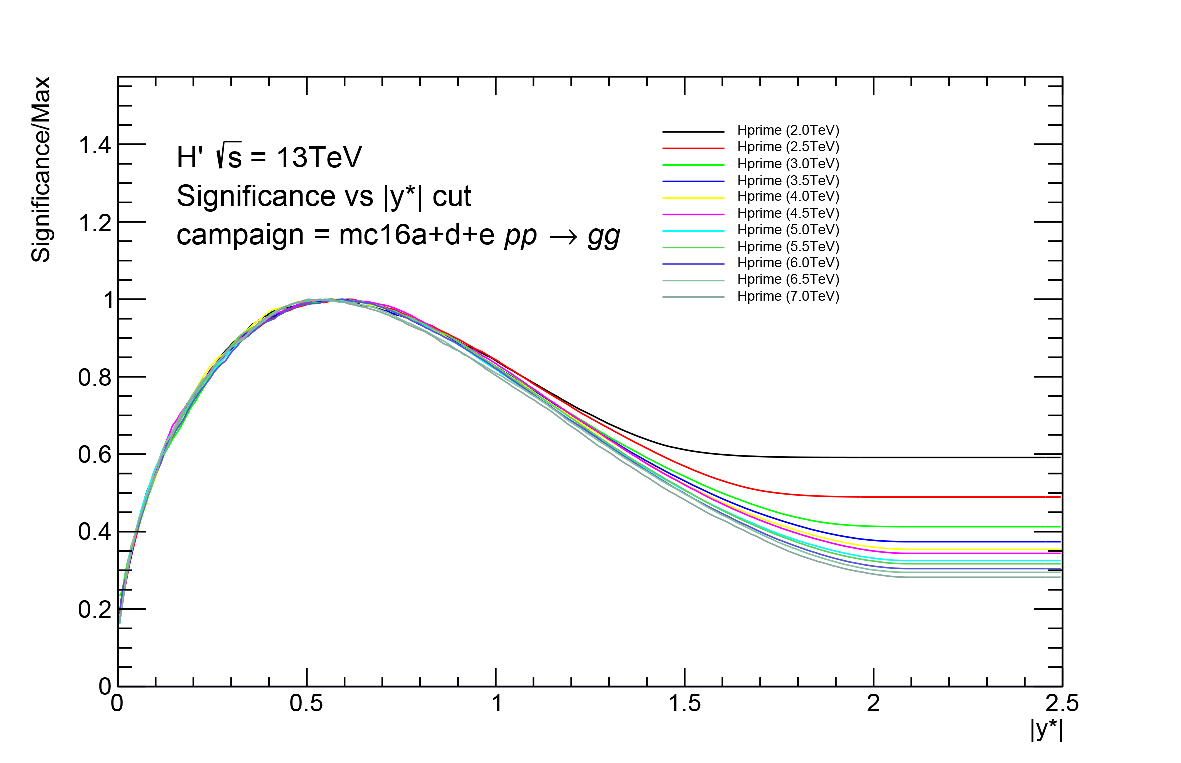
\includegraphics[width=0.45\columnwidth]{fig/yStarOptimization/New_Plots/Significance_Hprime_mc16a+d+e_gg.pdf}}
%        \caption{$H^\prime$ significance as a function \ystar\ cut in the case of (a) Inclusive, (b) $\geq$1 g-tag, (c) 2 g-tag.}
%        \label{fig: hprime significance as a function of y* cut}
%\end{figure}
% 
%
%\begin{table}[!htb]
%\begin{center}
%\begin{tabular}{ccccc}
%\toprule
%\multicolumn{1}{c}{$H^\prime$ Mass (TeV) } & \multicolumn{3}{c}{Optimal Selection} & \multicolumn{1}{c}{Peak Width} \\
%& \multicolumn{1}{c|}{Inclusive} & \multicolumn{1}{c|}{$\geq1$ $g$ tag} & \multicolumn{1}{c}{2 $g$ tag} \\
%\midrule
%2.0 & 0.57 & 0.57 & 0.57 & 0.50\text{--}0.65 \\
%2.5 & 0.58 & 0.59 & 0.62 & 0.50\text{--}0.67 \\
%3.0 & 0.59 & 0.59 & 0.59 & 0.50\text{--}0.66 \\
%3.5 & 0.56 & 0.56 & 0.60 & 0.49\text{--}0.65 \\
%4.0 & 0.58 & 0.58 & 0.58 & 0.47\text{--}0.65 \\
%4.5 & 0.55 & 0.57 & 0.57 & 0.35\text{--}0.68 \\
%5.0 & 0.55 & 0.56 & 0.57 & 0.47\text{--}0.66 \\
%5.5 & 0.55 & 0.55 & 0.57 & 0.46\text{--}0.66 \\
%6.0 & 0.60 & 0.60 & 0.60 & 0.52\text{--}0.66 \\
%6.5 & 0.55 & 0.55 & 0.54 & 0.47\text{--}0.64 \\
%7.0 & 0.56 & 0.56 & 0.51 & 0.35\text{--}0.61 \\
%\bottomrule
%\end{tabular}
%\end{center}
%\caption{$|y^*|$ selection leading to the maximum significance value calculated using Equation~\ref{eq:signifcanceYstar}.}\label{tab:ystarhprime}
%\end{table}

For String signal, there is also a dependence on $\cos\theta^{*}$, leads the \ystar\ will peak at 0 too. Figure.~\ref{fig: string significance as a function of y* cut} shows the significance of String signal as a function of \ystar\ cut. The maximum significance in all tagging categories are around 0.8, therefore an optimal $y^{*}$ cut for the String search is set to $|\ystar| < 0.8$. The exact values of \ystar\ cut that correspond to the peak significance value for the String signal at each mass point are shown in Table.~\ref{tab:ystarstring} with the ranges in \ystar\ cut around the peak that gives a significance $\geq$ 0.99.

\begin{figure}[!htb]
        \centering
        \subfloat[Inclusive]{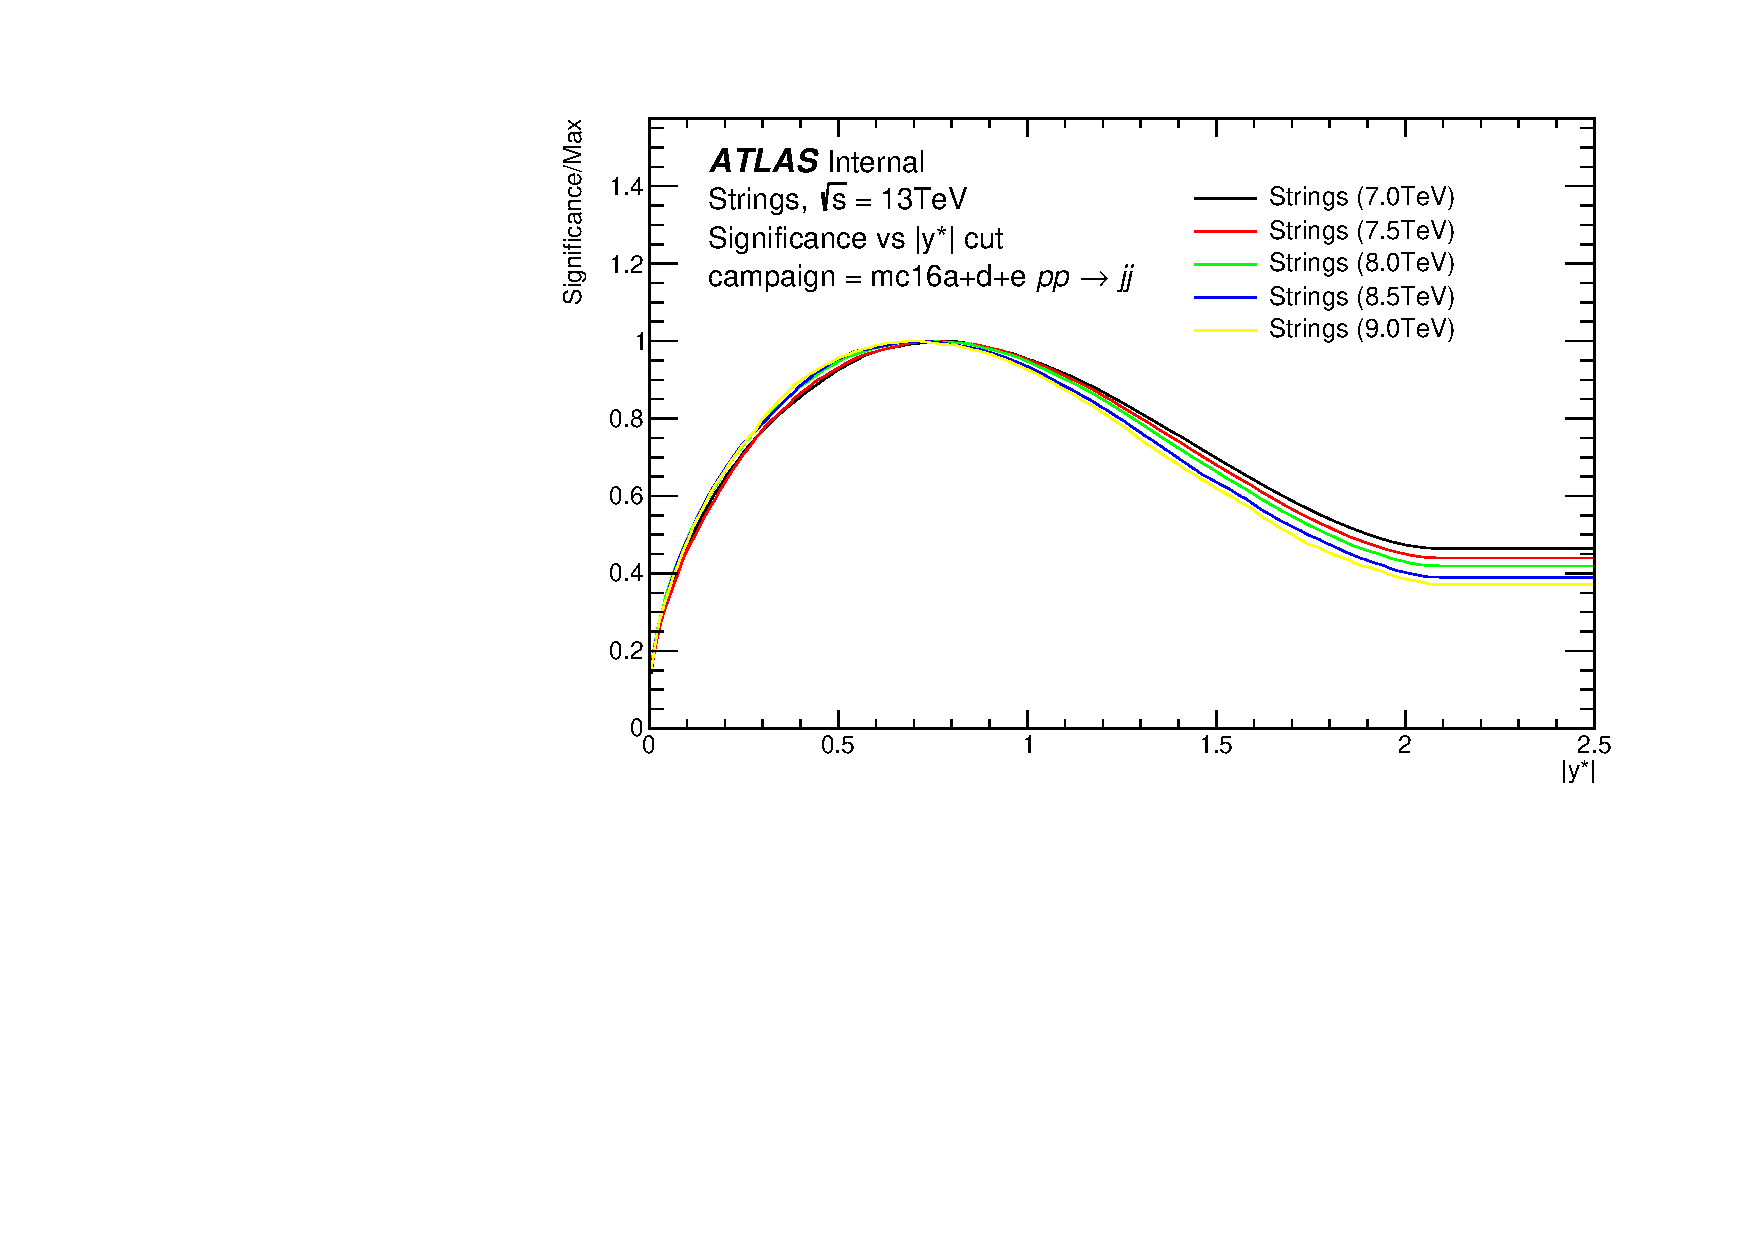
\includegraphics[width=0.45\columnwidth]{fig/yStarOptimization/New_Plots/Significance_Strings_mc16a+d+e_jj.pdf}}
        \subfloat[$\geq$1 g-tag]{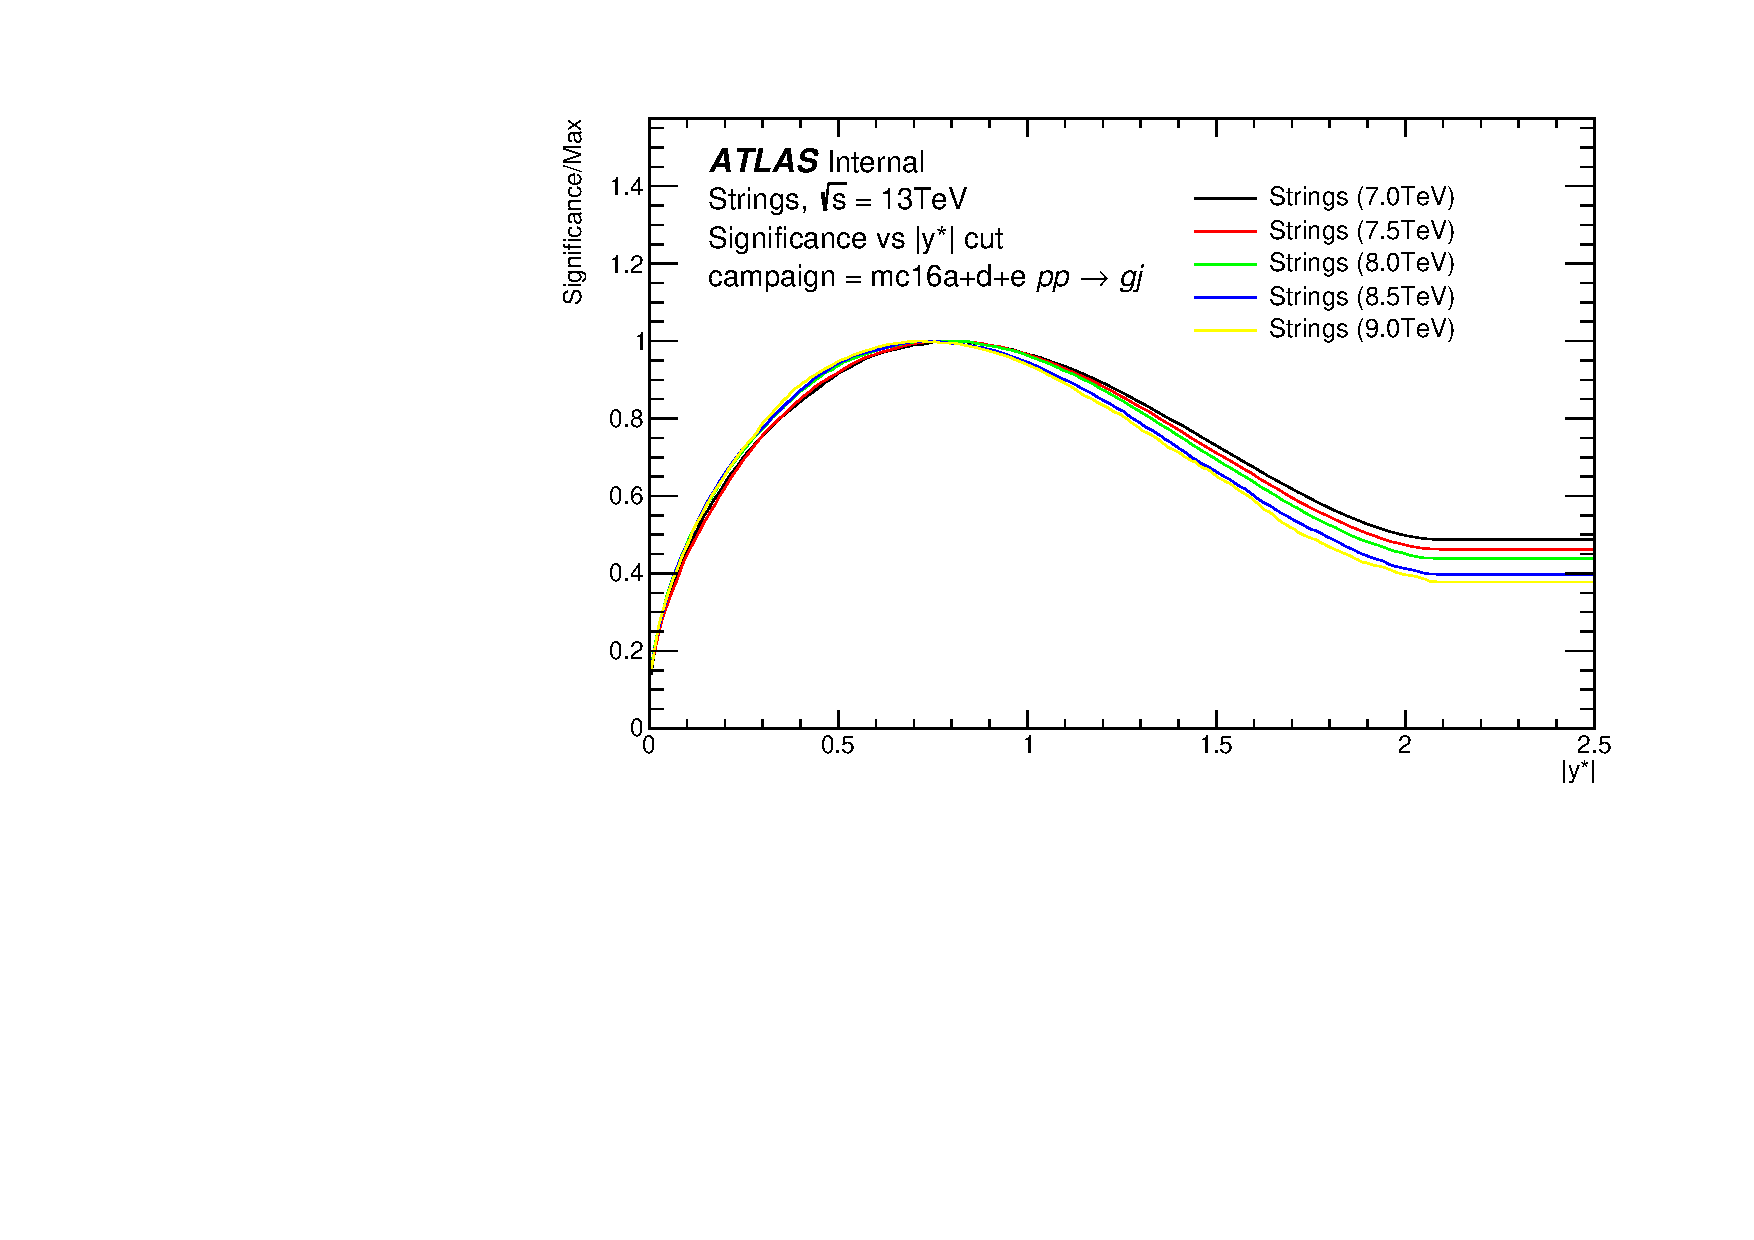
\includegraphics[width=0.45\columnwidth]{fig/yStarOptimization/New_Plots/Significance_Strings_mc16a+d+e_gj.pdf}}\\
        \subfloat[2 g-tag]{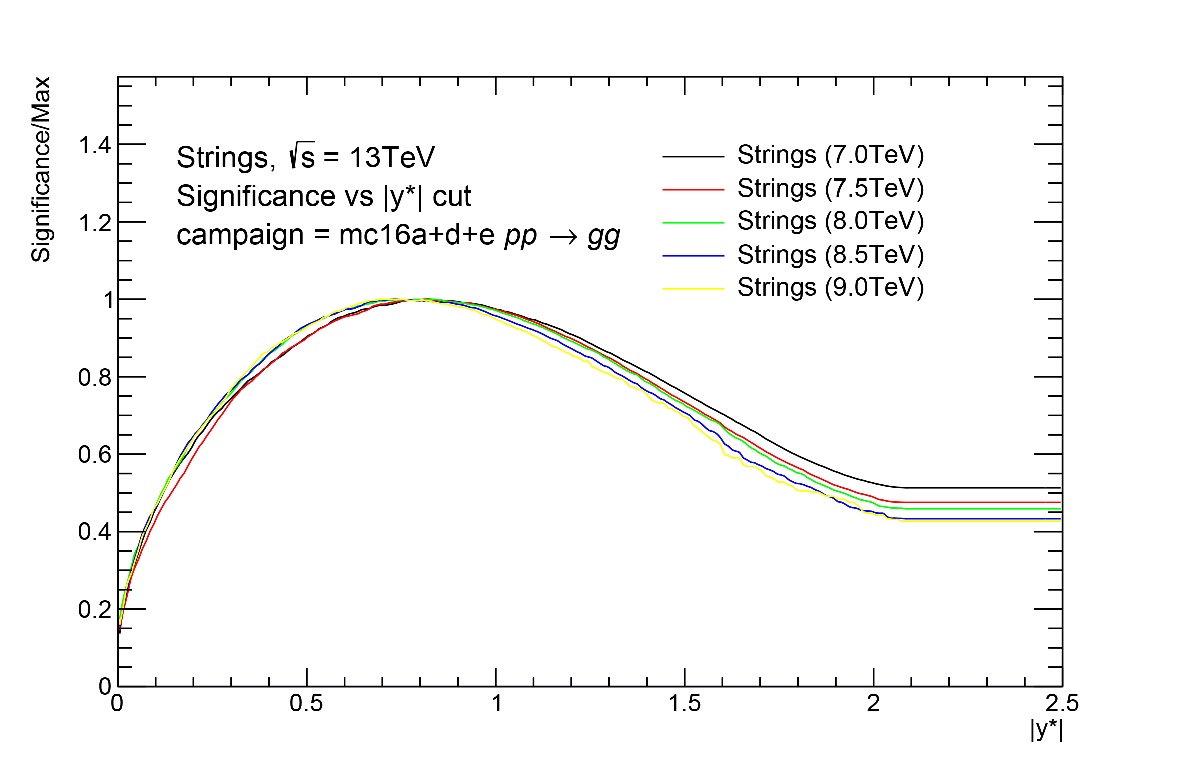
\includegraphics[width=0.45\columnwidth]{fig/yStarOptimization/New_Plots/Significance_Strings_mc16a+d+e_gg.pdf}}
        \caption{String significance as a function \ystar\ cut in the case of (a) Inclusive, (b) $\geq$1 g-tag, (c) 2 g-tag.}
        \label{fig: string significance as a function of y* cut}
\end{figure}


\begin{table}[!htb]
\begin{center}
\begin{tabular}{ccccc}
\toprule
\multicolumn{1}{c}{String Mass (TeV) } & \multicolumn{3}{c}{Optimal Selection} & \multicolumn{1}{c}{Peak Width} \\
& \multicolumn{1}{c|}{Inclusive} & \multicolumn{1}{c|}{$\geq1$ $g$ tag} & \multicolumn{1}{c}{2 $g$ tag} \\
\midrule
7.0 & 0.78 & 0.82 & 0.81 & 0.70\text{--}0.91 \\
7.5 & 0.77 & 0.77 & 0.83 & 0.68\text{--}0.91 \\
8.0 & 0.72 & 0.76 & 0.84 & 0.66\text{--}0.90 \\
8.5 & 0.74 & 0.74 & 0.74 & 0.65\text{--}0.85 \\
9.0 & 0.71 & 0.71 & 0.71 & 0.62\text{--}0.84 \\
\bottomrule
\end{tabular}
\end{center}
\caption{$|y^*|$ selection leading to the maximum significance value calculated using Equation~\ref{eq:signifcanceYstar}.}\label{tab:ystarstring}
\end{table}



Figure.~\ref{fig: graviton significance as a function of y* cut} shows the significance of Graviton signal as a function of \ystar\ cut. The significance peaks at about 0.6, so the optimal  cut for the Graviton search is $|\ystar| < 0.6$. Table.~\ref{tab:ystargraviton} shows the \ystar\ cut corresponding to the peak significance value for Graviton at each mass point, and the range in \ystar\ cut around the peak that gives a significance $\geq$ 0.99
\begin{figure}[!htb]
        \centering
        \subfloat[Inclusive]{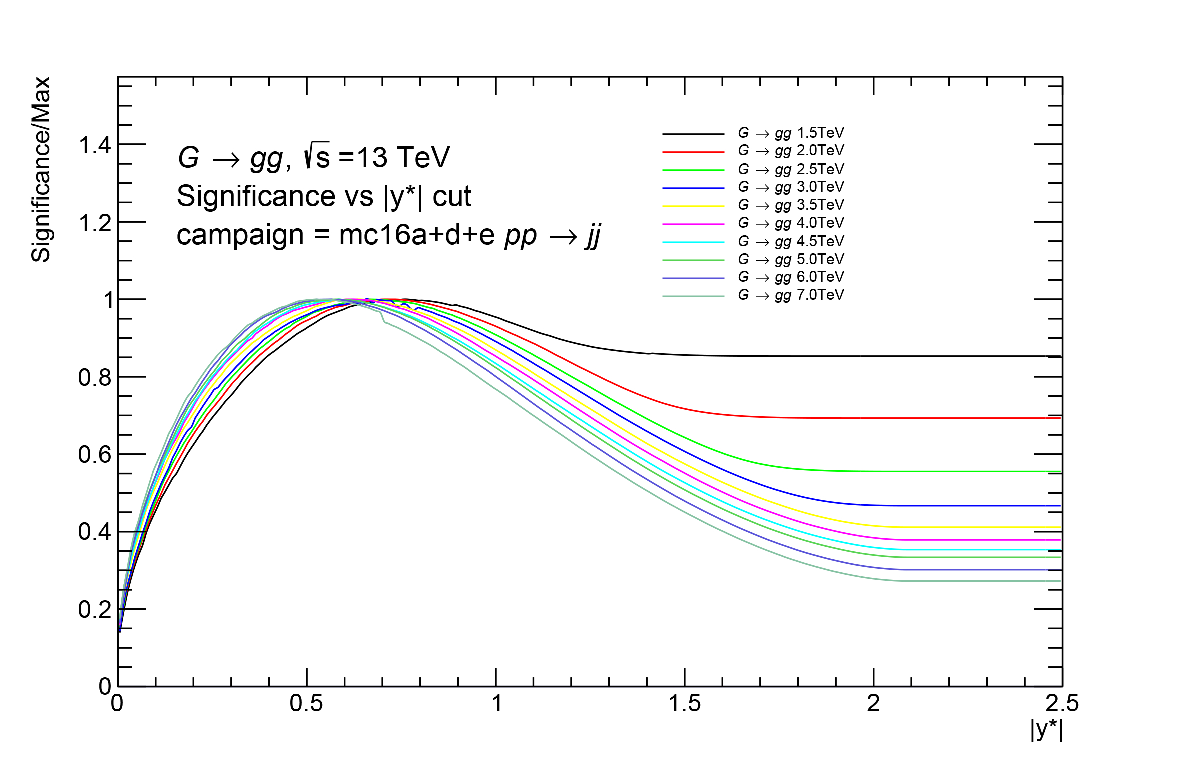
\includegraphics[width=0.45\columnwidth]{fig/yStarOptimization/New_Plots/Significance_Graviton_mc16a+d+e_jj.pdf}}
        \subfloat[$\geq$1 g-tag]{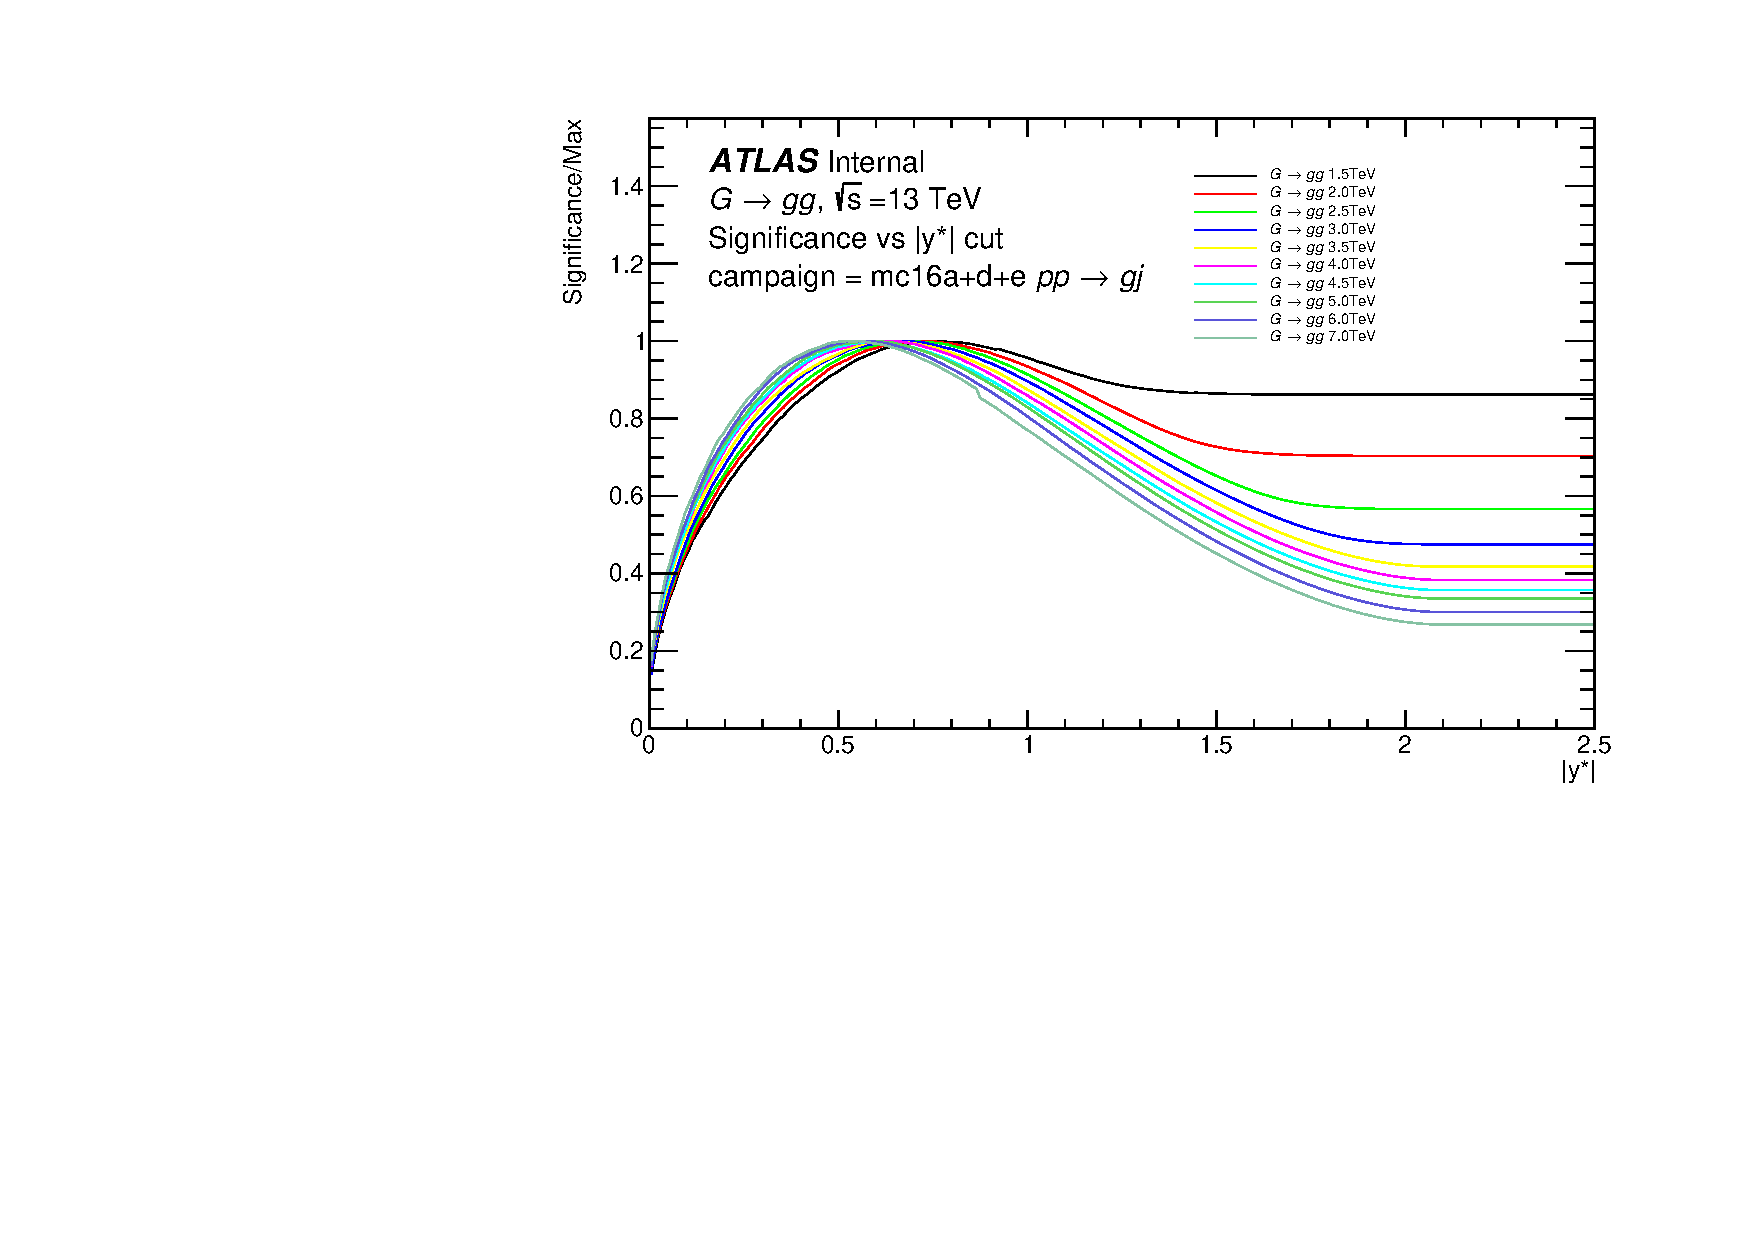
\includegraphics[width=0.45\columnwidth]{fig/yStarOptimization/New_Plots/Significance_Graviton_mc16a+d+e_gj.pdf}}\\
        \subfloat[2 g-tag]{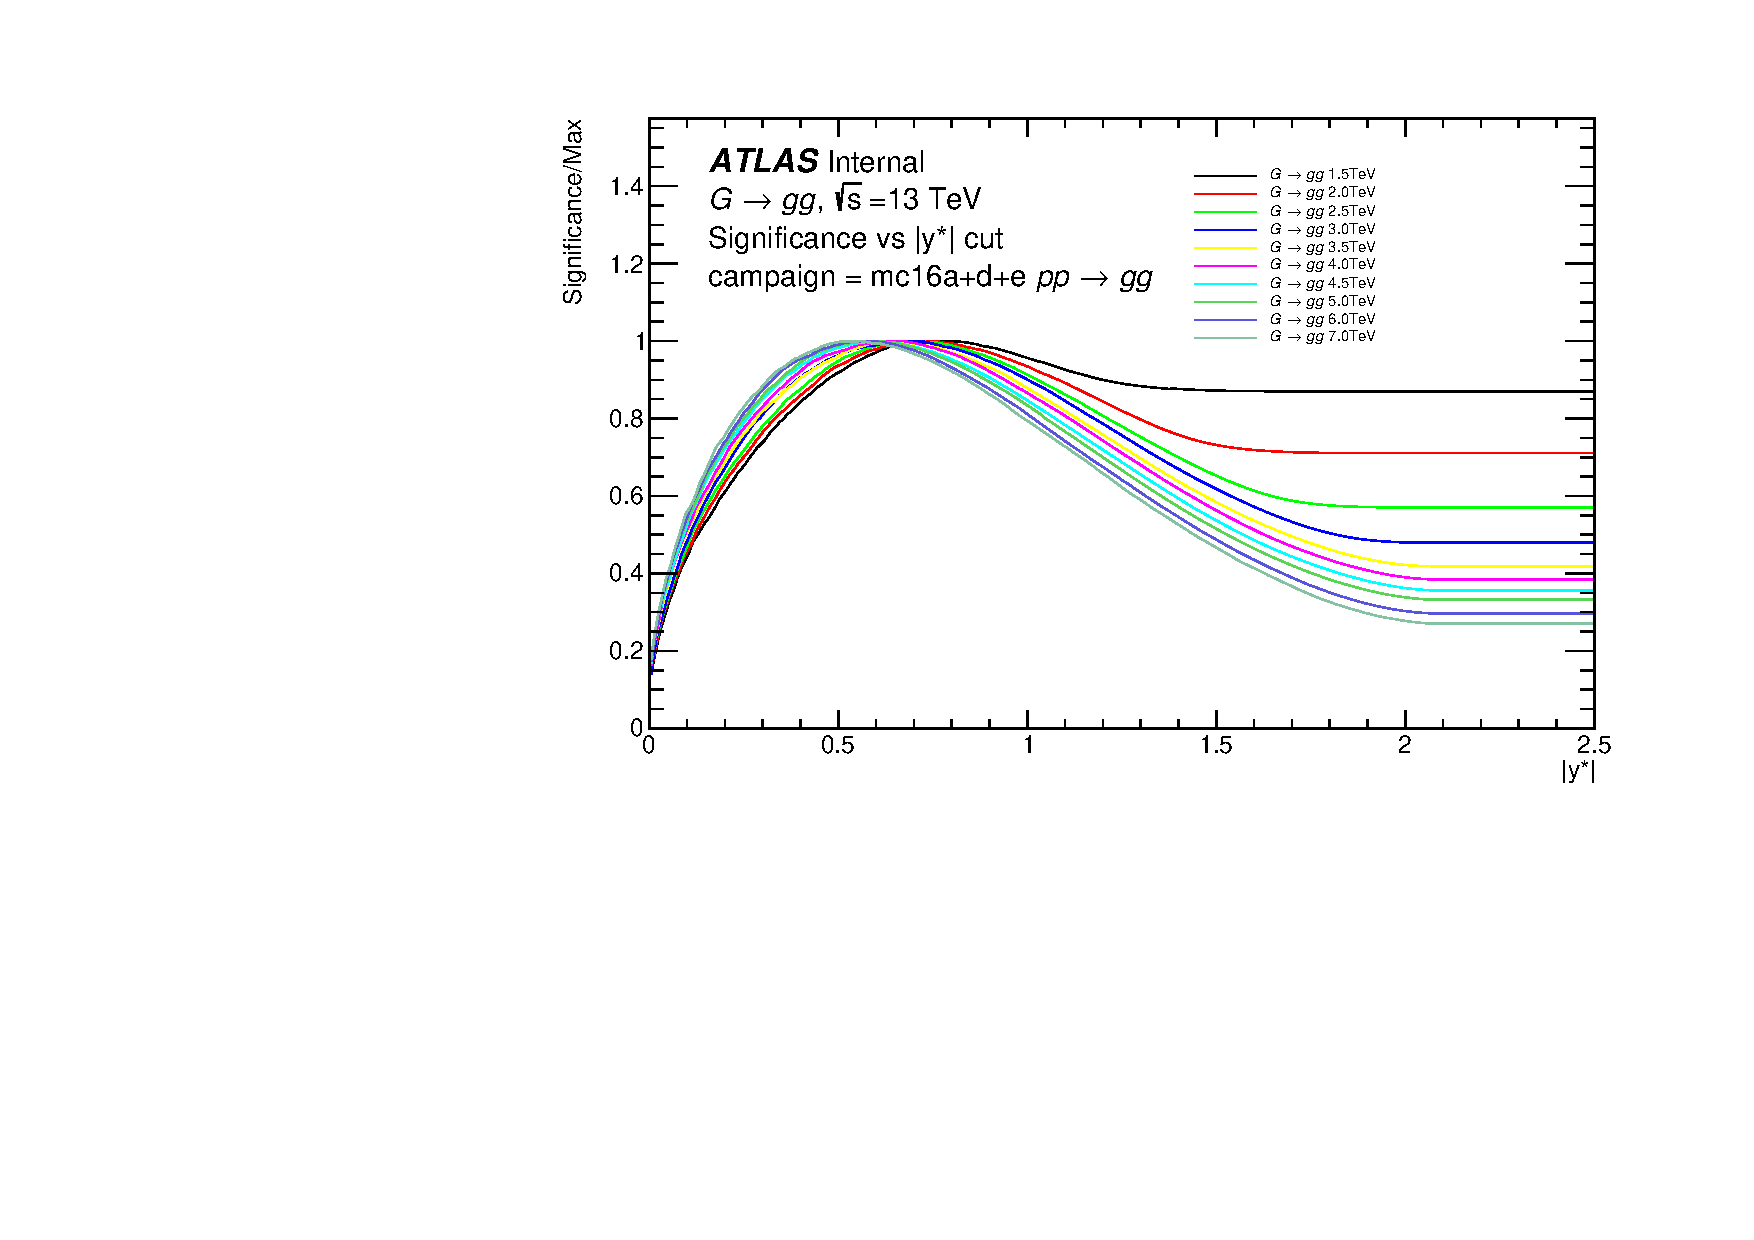
\includegraphics[width=0.45\columnwidth]{fig/yStarOptimization/New_Plots/Significance_Graviton_mc16a+d+e_gg.pdf}}
        \caption{Graviton significance as a function \ystar\ cut in the case of (a) Inclusive, (b) $\geq$1 g-tag, (c) 2 g-tag.}
        \label{fig: graviton significance as a function of y* cut}
\end{figure}


\begin{table}[!htb]
\begin{center}
\begin{tabular}{ccccc}
\toprule
\multicolumn{1}{c}{Graviton Mass (TeV) } & \multicolumn{3}{c}{Optimal Selection} & \multicolumn{1}{c}{Peak Width} \\
& \multicolumn{1}{c|}{Inclusive} & \multicolumn{1}{c|}{$\geq1$ $g$ tag} & \multicolumn{1}{c}{2 $g$ tag} \\
\midrule
1.5 & 0.77 & 0.77 & 0.78 & 0.65\text{--}0.87 \\
2.0 & 0.71 & 0.74 & 0.72 & 0.65\text{--}0.83 \\
2.5 & 0.67 & 0.69 & 0.70 & 0.61\text{--}0.80 \\
3.0 & 0.66 & 0.66 & 0.66 & 0.60\text{--}0.77 \\
3.5 & 0.64 & 0.65 & 0.65 & 0.57\text{--}0.73 \\
4.0 & 0.63 & 0.64 & 0.64 & 0.55\text{--}0.73 \\
4.5 & 0.59 & 0.59 & 0.59 & 0.53\text{--}0.69 \\
5.0 & 0.59 & 0.59 & 0.59 & 0.50\text{--}0.69 \\
6.0 & 0.57 & 0.57 & 0.60 & 0.49\text{--}0.66 \\
7.0 & 0.53 & 0.53 & 0.56 & 0.47\text{--}0.63 \\
\bottomrule
\end{tabular}
\end{center}
\caption{$|y^*|$ selection leading to the maximum significance value calculated using Equation~\ref{eq:signifcanceYstar}.}\label{tab:ystargraviton}
\end{table}



Figure.~\ref{fig: qbh significance as a function of y* cut} shows the significance of QBH signal as a function of \ystar\ cut. The maximum significance is at about 0.9, so the optimal cut for the QBH search is $|\ystar| < 0.9$. Table.~\ref{tab:ystarqbh} shows the \ystar\ cut corresponding to the peak significance value for the QBH at each mass point, and the range in \ystar\ cut around the peak that gives a significance $\geq$ 0.99
\begin{figure}[!htb]
        \centering
        \subfloat[Inclusive]{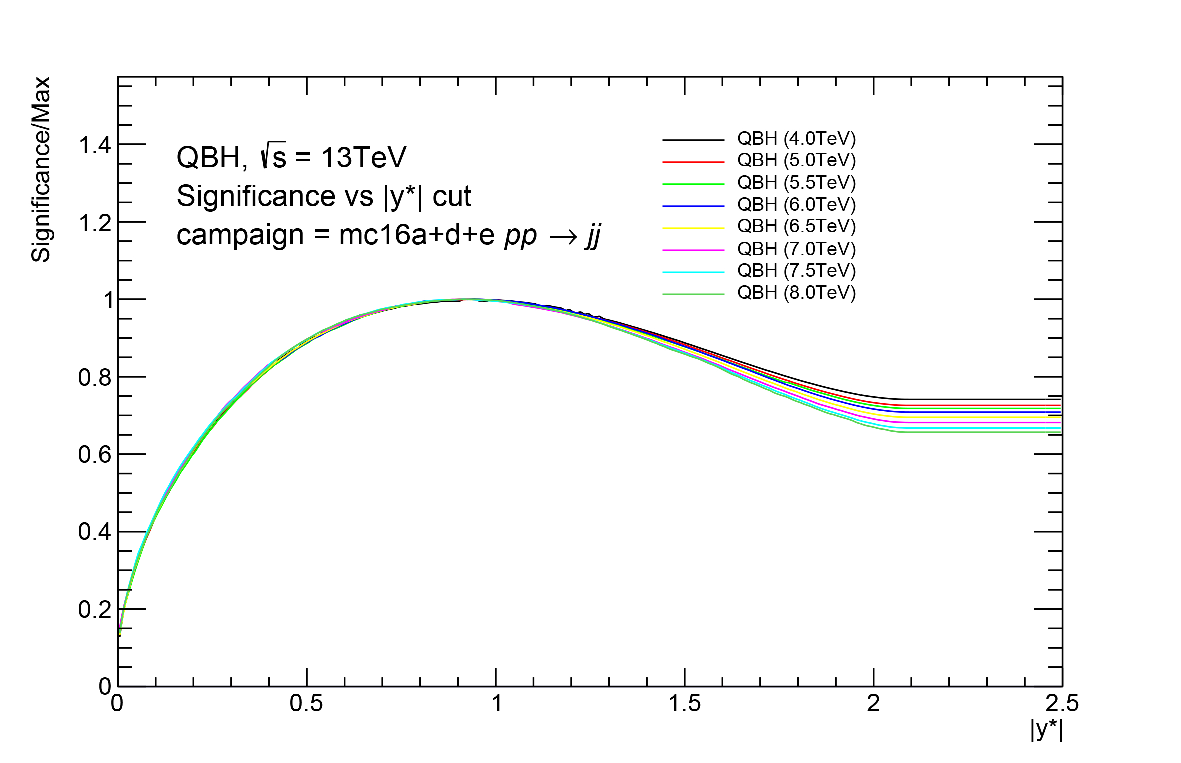
\includegraphics[width=0.45\columnwidth]{fig/yStarOptimization/New_Plots/Significance_QBH_mc16a+d+e_jj.pdf}}
        \subfloat[$\geq$1 g-tag]{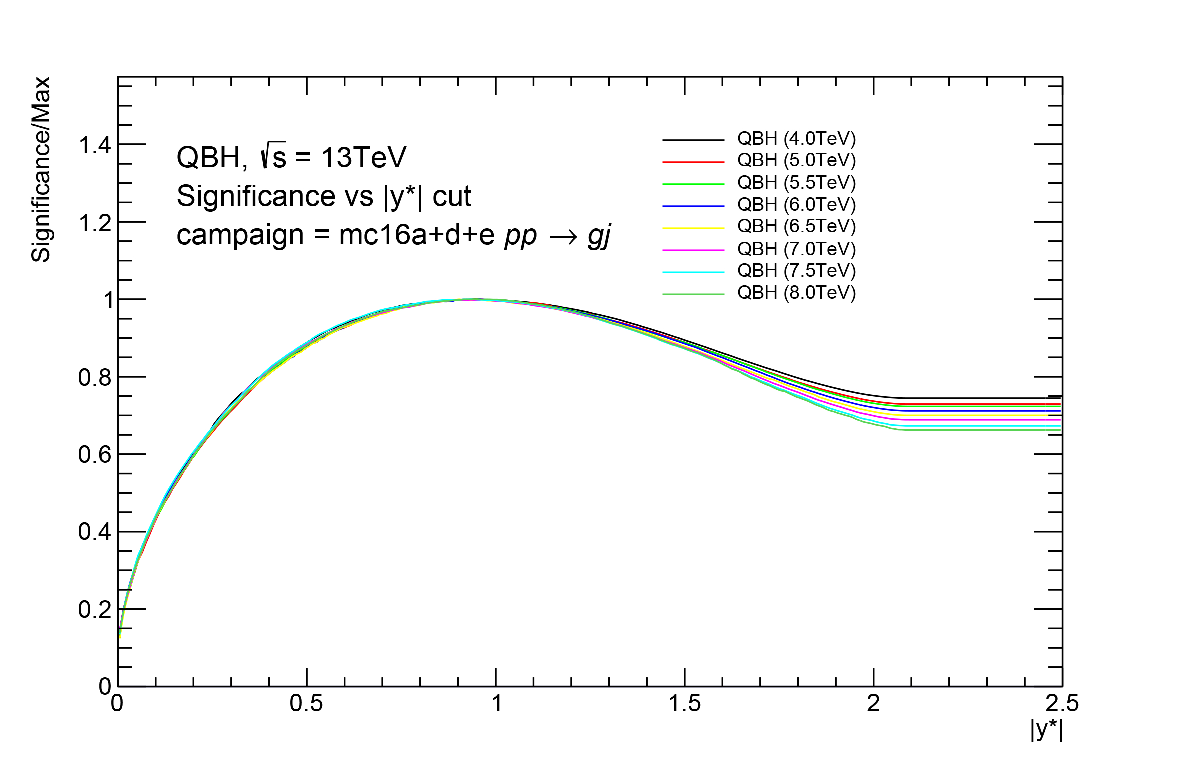
\includegraphics[width=0.45\columnwidth]{fig/yStarOptimization/New_Plots/Significance_QBH_mc16a+d+e_gj.pdf}}\\
        \subfloat[2 g-tag]{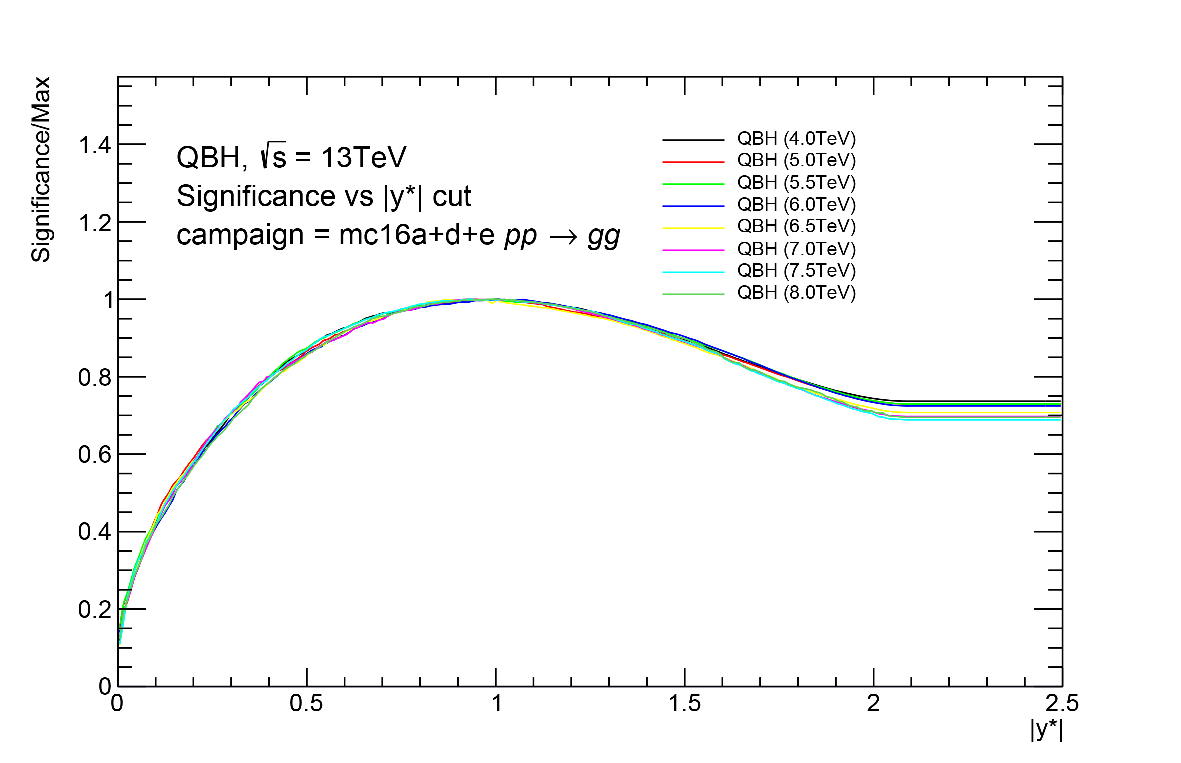
\includegraphics[width=0.45\columnwidth]{fig/yStarOptimization/New_Plots/Significance_QBH_mc16a+d+e_gg.pdf}}
        \caption{QBH significance as a function \ystar\ cut in the case of (a) Inclusive, (b) $\geq$1 g-tag, (c) 2 g-tag.}
        \label{fig: qbh significance as a function of y* cut}
\end{figure}


\begin{table}[!htb]
\begin{center}
\begin{tabular}{ccccc}
\toprule
\multicolumn{1}{c}{QBH Mass (TeV) } & \multicolumn{3}{c}{Optimal Selection} & \multicolumn{1}{c}{Peak Width} \\
& \multicolumn{1}{c|}{Inclusive} & \multicolumn{1}{c|}{$\geq1$ $g$ tag} & \multicolumn{1}{c}{2 $g$ tag} \\
\midrule
4.0 & 0.92 & 0.95 & 1.01 & 0.81\text{--}1.11 \\
5.0 & 0.95 & 0.95 & 0.95 & 0.81\text{--}1.09 \\
5.5 & 0.94 & 0.96 & 0.94 & 0.81\text{--}1.09 \\
6.0 & 0.92 & 0.96 & 1.01 & 0.81\text{--}1.09 \\
6.5 & 0.91 & 0.91 & 0.93 & 0.81\text{--}1.06 \\
7.0 & 0.93 & 0.97 & 0.94 & 0.82\text{--}1.07 \\
7.5 & 0.92 & 0.94 & 0.93 & 0.79\text{--}1.08 \\
8.0 & 0.92 & 0.96 & 0.99 & 0.82\text{--}1.09 \\
\bottomrule
\end{tabular}
\end{center}
\caption{$|y^*|$ selection leading to the maximum significance value calculated using Equation~\ref{eq:signifcanceYstar}.}\label{tab:ystarqbh}
\end{table}

\FloatBarrier

\subsubsection{Dijet Mass Turn-on}
\label{section:dijetmassturn-on} % uncomment if label used.

The \mjj\ turn-on is investigated by comparing events collected with the highest \pt\ 
trigger threshold with one with a lower \pt\ threshold using data. The efficiency of the HLT\_j420 trigger is calculated by comparing to the following triggers in each data taking period: 2015 HLT\_j360, 2016 HLT\_j380, 2017 and 2018 HLT\_mu50.  The muon trigger 2017 and 2018 are included as HLT\_j420 is the only unprescaled jet trigger available. The full Run 2 dataset is included for comparison as the HLT\_mu50 is available for all running periods. Events where the efficiency of trigger less than 99.5\% will be removed by a mass cut.


The efficiencies as a function of \mjj\ are shown in Figure.~\ref{fig: mass turn-on yStar 0.6} for $|\ystar|<0.6$ and Figure.~\ref{fig: mass turn-on yStar 0.8} for $|\ystar|<0.8$ in two gluon-tag categories for both triggers.  The results are summarised in Table.~\ref{table:massTurnOns} for the different data-taking periods. The \mjj~mass cut is chosen to be slightly above the value of the plateau ($\geq$99.5\%), so a cut of 1100 GeV
for $|\ystar|<0.6$ is applied. For $|\ystar|<0.8$, a cut of 1200 GeV is applied to samples with either one or two gluon tags.

\begin{figure}[htbp]
        \centering
        \subfloat[$\geq$1 g-tag]{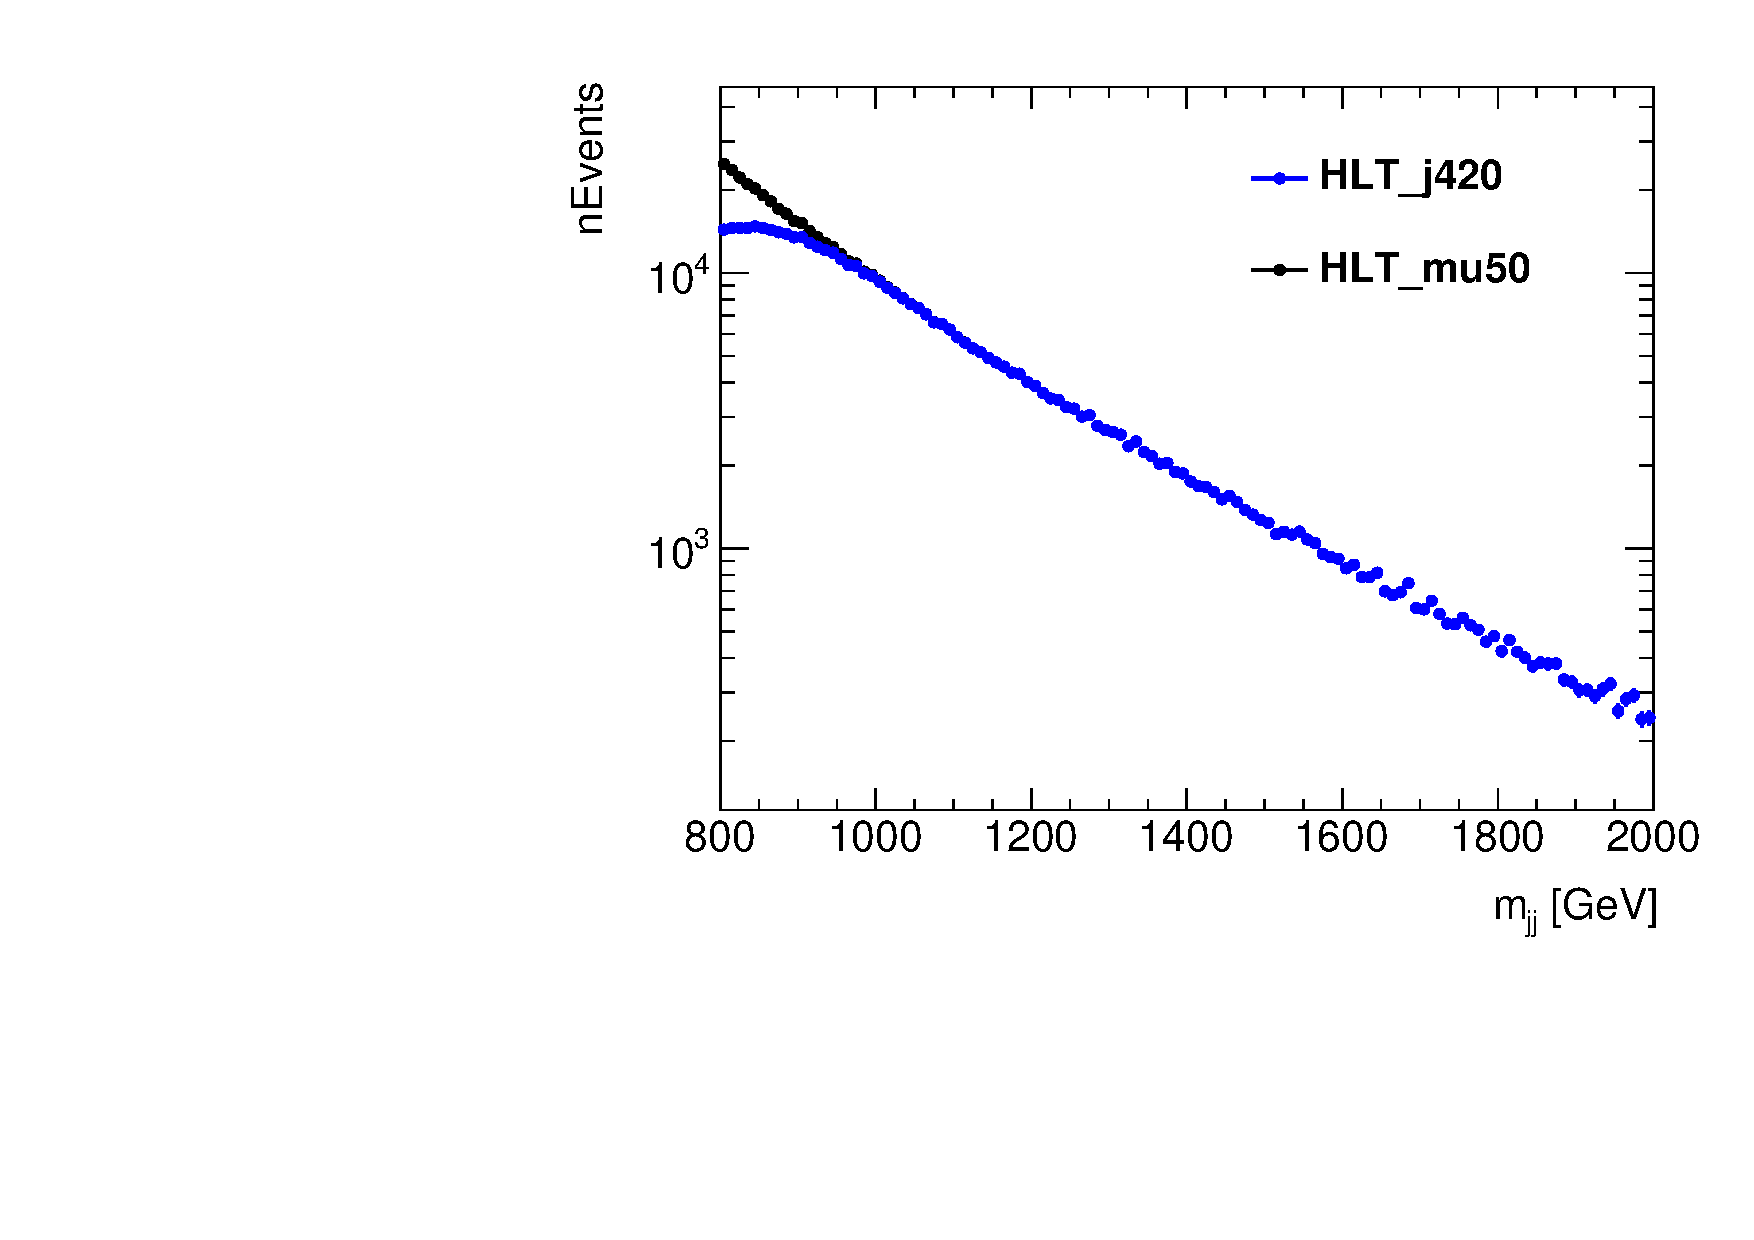
\includegraphics[width=0.5\columnwidth]{fig/massturnon/yStar0p6/mjj_turnon_1gluonTag_yStar0p6}}
        \subfloat[2 g-tag]{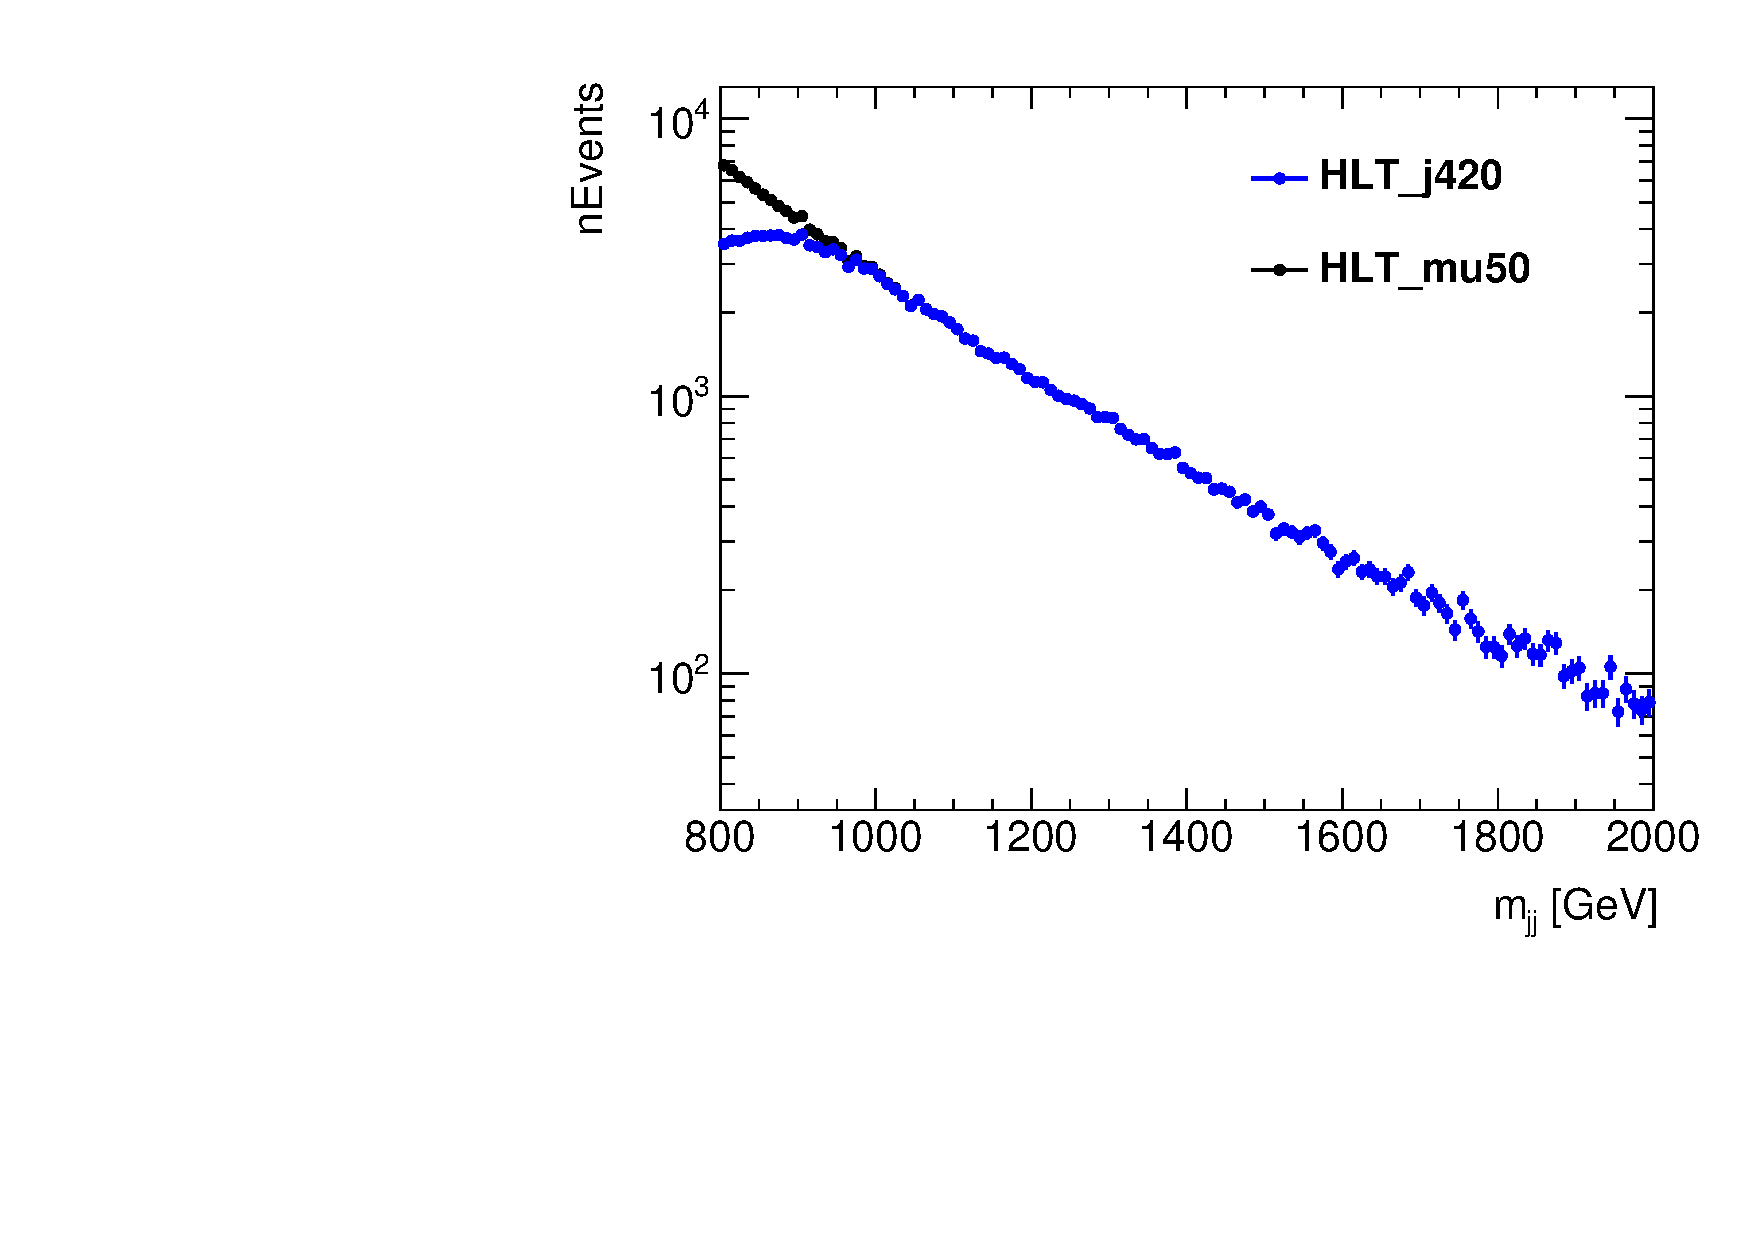
\includegraphics[width=0.5\columnwidth]{fig/massturnon/yStar0p6/mjj_turnon_2gluonTag_yStar0p6}}
        \\
        \subfloat[$\geq$1 g-tag]{\includegraphics[width=0.5\columnwidth]{fig/massturnon/yStar0p6/Ratio_mjj_turnon_1gluonTag_yStar0p6}}
        \subfloat[2 g-tag]{\includegraphics[width=0.5\columnwidth]{fig/massturnon/yStar0p6/Ratio_mjj_turnon_2gluonTag_yStar0p6}}
        
        \caption{Efficiencies as a function of \mjj\ for $|\ystar|<0.6$ using HLT\_j420 compared with HLT\_mu50 in the case of comparison of mass spectra with 
        (a) $\geq$1 g-tag, (b) 2 g-tag and the ratio between the two (c) $\geq$1 g-tag and (d) 2 g-tag.}
        \label{fig: mass turn-on yStar 0.6}
\end{figure}

\begin{figure}[htbp]
        \centering
        \subfloat[$\geq$1 g-tag]{\includegraphics[width=0.5\columnwidth]{fig/massturnon/yStar0p8/mjj_turnon_1gluonTag_yStar0p8}}
        \subfloat[2 g-tag]{\includegraphics[width=0.5\columnwidth]{fig/massturnon/yStar0p8/mjj_turnon_2gluonTag_yStar0p8}}
        \\
        \subfloat[$\geq$1 g-tag]{\includegraphics[width=0.5\columnwidth]{fig/massturnon/yStar0p8/Ratio_mjj_turnon_1gluonTag_yStar0p8}}
        \subfloat[2 g-tag]{\includegraphics[width=0.5\columnwidth]{fig/massturnon/yStar0p8/Ratio_mjj_turnon_2gluonTag_yStar0p8}}
        \caption{Efficiencies as a function of \mjj\ for $|\ystar|<0.8$ using HLT\_j420 compared with HLT\_mu50 in the case of comparison of mass spectra with 
        (a) $\geq$1 g-tag, (b) 2 g-tag and the ratio between the two (c) $\geq$1 g-tag and (d) 2 g-tag.}
        \label{fig: mass turn-on yStar 0.8}
\end{figure}

\begin{table}[h]
	\centering 
	\resizebox{0.95\textwidth}{!}{
	\begin{tabular}{SSSSS}
		\toprule
		\multicolumn{1}{c}{Data Taking Period}  &  \multicolumn{2}{c}{Mass turn on $|\ystar|<0.6$ } &  \multicolumn{2}{c}{Mass turn on $|\ystar|<0.8$ } \\
		& \multicolumn{1}{c}{$\geq$1 g-tag ( GeV )} &  \multicolumn{1}{c}{2 g-tag ( GeV )} 
		& \multicolumn{1}{c}{$\geq$1 g-tag ( GeV )} &  \multicolumn{1}{c}{2 g-tag ( GeV )}  \\
		\midrule 
		2015  & 1040 & 1030 & 1160 & 1160 \\
		2016  & 1030 & 1030 & 1160 & 1170 \\
		2017  & 990 & 1000  & 1110 & 1120 \\
		2018  & 1000 & 1010  & 1110 & 1120 \\
		\multicolumn{1}{c}{Run~2} & 1020 & 1030 & 1120 & 1120 \\
		\bottomrule
	\end{tabular}}
	\caption{ The \mjj value of the start of the plateau ($\geq$99.5\%) for each period of data taking. 
		\label{table:massTurnOns}
	}
\end{table}

\FloatBarrier
\subsubsection{Optimised Selection}
\label{sec:analysiscuts}

In addition to the baseline selection described in Section~\ref{sec:base_selection}, optimized cuts are  applied to different tagging regions to improve the search potential with good tracking efficiency. 

The following additional cuts are applied for the the inclusive samples.
\begin{itemize}
	\item $|\ystar| < 0.8$
	\item \mjj > 1200 GeV
\end{itemize}

The following additional cuts are for quark-gluon tagging.
\begin{itemize}
	\item $|\eta| < 2.1$ (both jets) for track acceptance
	\item $\ge 1$ gluon tagged (75\% working point)
	\item 2 gluons tagged (75\% working point)
\end{itemize}
where the 75\% gluon selection criteria is applied as: $\ntrk~> -7.3 +
4.2\ln(\pt)$, with jet \pt\ in GeV.


\FloatBarrier

The acceptance times efficiency as a function of signal masses in inclusive, signal-gluon and double-gluon
tagged regions for different benchmark signal models are shown in Figure~\ref{fig:AccxEff}.

\begin{figure}[htb]
 \centering
 \includegraphics[width=0.5\textwidth]{fig/benchmark_signals/AccxEff_strings.pdf}
 \caption{Acceptance times efficiency for the String signal.}
 \label{fig:AccxEff}
\end{figure}
\FloatBarrier
\subsubsection{Selected Kinematic Plots}
%\label{sec:kinematic_distributions} % uncomment if label used.

In this section a selection of kinematic and monitoring plots processed with samples passed the gluon-gluon selection criteria are shown in Figure~\ref{fig:GGmonitoring1}, \ref{fig:GGmonitoring2}, \ref{fig:GGmonitoring3}. The distributions of kinematics in MC are consistent with full dataset.

\begin{figure}[htb]
 \centering
 \subfloat[] {\includegraphics[width=0.5\textwidth]{fig/monitoring/GG/newStudy_HT_logY_v01.pdf}}
 \subfloat[] {\includegraphics[width=0.5\textwidth]{fig/monitoring/GG/newStudy_NPV_logY_v01.pdf}}\\
 \subfloat[] {\includegraphics[width=0.5\textwidth]{fig/monitoring/GG/newStudy_averageInteractionsPerCrossing_logY_v01.pdf}}
  \subfloat[] {\includegraphics[width=0.5\textwidth]{fig/monitoring/GG/newStudy_njets_logY_v01.pdf}}
 \caption{Monitoring plots for %2016 data, 
 the gluon-gluon selection. (a) scalar \pt~sum of all parton-level jets ($H_T$), %(b) $MH_T$ (missing transverse momentum calculated only from the jets in the event), 
 (b) number of primary interaction vertices (NPV),
 (c) average interactions per bunch crossing, and 
 (d) number of jets.}
 \label{fig:GGmonitoring1}
\end{figure}

 \begin{figure}[htb]
 \centering
 \subfloat[] {\includegraphics[width=0.5\textwidth]{fig/monitoring/GG/newStudy_deltaPhi_logY_v01.pdf}}
 \subfloat[] {\includegraphics[width=0.5\textwidth]{fig/monitoring/GG/newStudy_jet_eta_logY_v01.pdf}}\\
 \subfloat[] {\includegraphics[width=0.5\textwidth]{fig/monitoring/GG/newStudy_jet_phi_logY_v01.pdf}}
  \subfloat[] {\includegraphics[width=0.5\textwidth]{fig/monitoring/GG/newStudy_jet_rapidity_logY_v01.pdf}}
 %
  \caption{Monitoring plots on the gluon-gluon sample. 
  (a) $\Delta\phi$ between the two jets,
  (b) jet $\eta$,
  (c) jet $\phi$, and 
  (d)  jet rapidity.  %Fluctuations in the jet $phi$ distribution are attributable to dead modules in the tile calorimeter which lead to fewer jets in small slices of the detector.
  }
 \label{fig:GGmonitoring2}
\end{figure}


 \begin{figure}[htb]
 \centering
 %
 \subfloat[] {\includegraphics[width=0.5\textwidth]{fig/monitoring/GG/newStudy_jet_pt_logY_v01.pdf}}
 %
 %\subfloat[] {\includegraphics[width=0.45\textwidth]{fig/monitoring/GG/newStudy_yBoost_logY_v01.pdf}}
 \subfloat[] {\includegraphics[width=0.5\textwidth]{fig/monitoring/GG/newStudy_yStar_logY_v01.pdf}}
 \caption{Monitoring plots on  the gluon-gluon sample.
 (a) jet \pt,
  %(b) \yB{}, and
  (b) \ystar{}. }
 \label{fig:GGmonitoring3}
\end{figure}


\clearpage


\clearpage

\subsection{Analysis framework}
%\label{sec:statistical} % uncomment if label used. 
\label{sec:statistical_framework}

\subsubsection{Fitting framework}

The fitting framework used to parameterise QCD background is based on XML Analytic Workspace Builder~\cite{xmlAnaWSBuilder} (xmlAnaWSBuilder), which employs one-dimensional 
observables to create RooFit~\cite{RooFit} workspaces. The workflow of the framework is summarised in Figure~\ref{fig:xmlAnaWSBuilderworkflow}.

\begin{figure}[htb]
 \centering
\includegraphics[width=0.75\textwidth]{fig/06-StatisticalFramework/xmlAnaWSBuilder_workflow}
\caption{Workflow of the XmlAnaWSBuilder.  \label{fig:xmlAnaWSBuilderworkflow}}
\end{figure}

The xRooFit framework~\cite{xRooFit} that based on RooFit data fitting package is used for data fitting. Modifications are needed so that it can integrate over binned data, as RooFit evaluates its fit functions using the centre value of each bin rather than the actual average mass in each bin. As a result, significant biases could occur in the fit results~\cite{gligorov2021avoiding}. Recent developments introduce a new class of \texttt{RooBinSamplingPdf} in to RooFit package, which solve such issue.

% in RooFit have created a new class, \texttt{RooBinSamplingPdf}, which can now be used to avoid this problem which is available in a patch to ROOT v6.23~\cite{RooBinSamplingPdf} and built in the v6.24 release. 

%%%%%%%%%%%%%%%%%%%%%%%%%%%%%%%%%%%%%%%%%%%%%%%%%%%%%%%%%%%%%%%%%%%%%% 
%\subsection{Likelihood Definition}
%
%The statistical analysis of the data uses a binned likelihood function~\cite{AlKhoury:2692011} which maximum correspond to the
%best description of data. It is defined as the product over all bins of the Poisson probability to observe $N^{\mathrm{obs}}_i$
%data events given a prediction of $N^{\mathrm{exp}}_i (\mu, \theta)$ events in a certain bin $i$:
%\begin{equation}
%  L (\mu, \theta) = 
%  \prod_{i \in \mathrm{bins}} 
%  \frac{ \left[N^{\mathrm{exp}}_i (\mu,  \theta)\right]^{N^{\mathrm{data}}_i}} {N^{\mathrm{data}}_{i}!}
%  \exp\left[ - N^{\mathrm{exp}}_i (\mu,  \theta) \right]
%%\label{Eq:fitfunction}% uncomment if label used. 
%\end{equation}
%In this likelihood, the number of predicted events is made dependent on two sets of parameters: the signal strength $\mu$ 
%and the  nuisance parameters $\mathbf{\theta} = {\theta_1, \cdots, \theta_l}$, as follows
%
%\begin{equation}
%N^{\mathrm{exp}}_i (\mu,  \theta) = \mu N^{\mathrm{exp}}_{i,\mathrm{sig}}(\mathbf{\theta}) +  N^{\mathrm{exp}}_{i,b}(\mathbf{\theta}).
%%\label{Eq:fitfunction}% uncomment if label used. 
%\end{equation}
%The parameter of interest, $\mu$, is a scale factor for the signal being searched for. The expected number of background 
%events, $N^{\mathrm{exp}}_{i,b}(\mathbf{\theta})$, is measured using functions described in the next sub section where the nuisance
%parameters (NP) are the function parameters. 
%
%The nuisance parameters (NP) $\theta_i$ encode the dependence of the prediction on systematic uncertainties
%into continuous parameters in the likelihood. The prior knowledge on these parameters is reflected by a
%Gaussian penalty term Gauss$(0 | \theta_i,1)$ included in to the likelihood for each NP, rending displacement of these
%parameters depreciated. The parameters $\theta_i$ are therefore expressed in standard deviation in the following.
%It results in a log-normal (normal) dependence of the predicted rates (shapes) on the displayed parameter
%values.
%
%The nominal fit result in terms of $\mu$ and $q_\mu$  is obtained by maximizing the likelihood function with respect
%to all parameters. This is referred to as the maximized log-likelihood value, MLL. The profile likelihood
%ratio test statistic, $q_\mu$ is then constructed as follows:
%\begin{equation}
%q_\mu = 2 \ln \left[ \cal{L}(\mu, \hat{\hat{\mathbf{\theta}}}_\mu) / \cal{L}(\hat{\mu}, \hat{\mathbf{\theta}}_\mu)  \right] 
%\end{equation}
%where $\hat{\mu}$ and $\hat{\mathbf{\theta}}_\mu$ are the parameters that maximise the likelihood 
%(with the constraint $0  \le \hat{\mu} \le \mu$), , and 
%$\hat{\hat{\mathbf{\theta}}}_\mu$ are the nuisance parameter values that maximise the likelihood for a given $\mu$. 
%This test statistic is used to measure the compatibility of the background-only model with the observed data, 
%extracting the local $p_0$
%value, and, if no hint of a signal is found in this procedure, for the derivation of exclusion intervals using
%the \textit{CLs} method.
%%~\cite[Cowan:2010js, Read:2002hq]. 
%%%%%%%%%%%%%%%%%%%%%%%%%%%%%%%%%%%%%%%%%%%%%%%%%%%%%%%%%%%%%%%%%%%%%%%%%%%%%%%
\subsubsection{Statistical method} 

In this analysis, the discriminating variable is set to the dijet invariant mass $m_{jj}$, and the distribution of it is used as  a probability density function (pdf) to build the likelihood function.

\paragraph{Parametric background models}\mbox{}\par
%\subsubsection{Parametric background and signal models}

%The string signals are parameterized as the convolution of an
%exponential, $\lambda_c \exp\left( -\lambda_c m_{jj} \right)$, and a
%Gaussian,  $G(m_{jj};\mu_c,\sigma_c)$, added to an another Gaussian
%$G(m_{jj};m_G,\sigma_G)$. 
%The two terms are weighted by the parameter $a$:

%\begin{eqnarray}
%f_s(m_{jj};\bm{p}_s) & = &
%f_s(m_{jj};a,\lambda_c,\mu_c,\sigma_c,m_G,\sigma_G) = a
%G(m_{jj};m_G,\sigma_G) \nonumber \\ 
%& + & (1 - a) \frac{\lambda_c}{2} \exp \left[
%-\lambda_c \left( m_{jj} - \mu_c - \frac{\lambda_c \sigma_c^2}{2} 
%\right) \right] 
%\mathrm{erfc} \left( 
%\frac{ m_{jj} - \mu_c - \lambda_c\sigma_c^2}{\sqrt{2}\sigma_c}
%\right)\, .
%\end{eqnarray}

%\noindent
%The parameter $a$ is typically fixed, and $\bm{p}_s$ are free parameters
%determined by fitting to MC signal templates. 
%\textit{We may have moved to using the template histograms directly, but
%I keep this parametric description in for a while longer.} 

The distribution of \mjj~of background is parameterized by

\begin{equation}\label{pdfb}
f_b(m_{jj};\bm{p}_b) = f_b(m_{jj};p_1,p_2,p_3,p_4,p_5) = p_1 \left( 1
- \frac{m_{jj}}{\sqrt{s}} \right)^{p_2} \left( \frac{m_{jj}}{\sqrt{s}}
\right)^{p_3 + p_4\ln\left( \frac{m_{jj}}{\sqrt{s}} \right) +  p_5
  \left[ \ln \left( \frac{m_{jj}}{\sqrt{s}} \right) \right]^2}\, .  
\end{equation}

\noindent
where $\bm{p}_b$ are free parameters determined by fitting to data (or 
pseudo data), and $\sqrt{s} = 13$~TeV.
In some cases, $p_5 = 0$ is taken. 
We will assume Equation~(\ref{pdfb}) is normalized to unity as needed.

Given that we are employing a binned likelihood approach and working with histograms, it becomes essential to determine the average count of events in the $i$th bin, arising from both the signal and background contributions:

\begin{eqnarray}
s_i & = & s_\mathrm{tot} \int_{\mathrm{bin}\ i} f_s(m_{jj};\bm{p}_s)
dm_{jj}\, .\\
b_i & = & b_\mathrm{tot} \int_{\mathrm{bin}\ i} f_b(m_{jj};\bm{p}_b) dm_{jj}\, .
\end{eqnarray}

\noindent
where $f_s$ and $f_b$ are pdfs of $m_{jj}$ for the signal and
background, respectively. 
The quantities $s_\mathrm{tot}$ and $b_\mathrm{tot}$ represent the total mean
numbers of signal and background events.
The variable $b_\mathrm{tot}$ is an additional nuisance parameter.
The signal normalization $s_\mathrm{tot}$ is  not treated as a parameter that can be adjusted, but rather is set to the value determined by the nominal signal model. 
The parameter can be expressed as $s_\mathrm{tot} = \sigma L \varepsilon$,
where $\sigma$ is fixed by the model cross section, and $L$ and
$\varepsilon$ represent the nominal luminosity and total acceptance times
efficiency, respectively.


\paragraph{Uncertainties}\mbox{}\par
\label{sec:unc}

In this analysis, there are six sources of systematic uncertainties on the signal studied: 

\begin{description}
\item $\delta L$ an uncertainty on the integrated luminosity of the data
  sample,
\item $\delta\varepsilon$ an uncertainty on the signal efficiency times
  acceptance, 
\item $\delta t$ an uncertainty on the gluon-tag efficiency,
\item $\delta E_\mathrm{JER}$ an uncertainty on the jet energy
  resolution.
\item $\delta E_\mathrm{JES}$ an uncertainty on the jet energy scale.
\item $\delta S$ an uncertainty due to spurious signals.
\end{description}

\noindent
All these uncertainties are treated as shape uncertainties except for
$\delta L$ which is a normalization uncertainty.
These uncertainties are associated to nuisance parameters denoted by
$\alpha_L$,
$\alpha_\varepsilon$, $\alpha_t$, $\alpha_{E_\mathrm{JER}}$,
$\alpha_{E_\mathrm{JES}}$, $\alpha_S$, 
respectively, and the values of the auxiliary measurements by 
$\theta_b$, $\theta_L$, $\theta_\varepsilon$, $\theta_t$,
$\theta_{E_\mathrm{JER}}$, $\theta_{E_\mathrm{JES}}$, $\theta_S$, respectively.


\paragraph{Likelihood function definition}\mbox{}\par

A binned likelihood is used in this analysis. Consider the $m_{jj}$ histogram of $\bm{n} = (n_1, \ldots, n_N)$
events, the likelihood function without uncertainties is built as:
\begin{equation}
\mathcal{L}(\mu;b_\mathrm{tot},\bm{p}_s,\bm{p}_b) = \prod_{i=1}^N \frac{(\mu s_i +
b_i)^{n_i}}{n_i!} e^{-(\mu s_i + b_i)}\, .
\end{equation}
\noindent
where the parameter of interest (POI) $\mu$ is the signal strength
parameter, $b_i$ is the number of background events in the $i$ bin, $s_i$ is the number of signal events in the $i$ bin. Background-only
hypothesis corresponding to $\mu = 0$, whereas nominal signal hypothesis corresponding to $\mu = 1$.

The full likelihood function with uncertainties included is defined as:
%Including uncertainties, the full likelihood function is\footnote{To be succinct, the bin index on the arguments of the functions $N_i$ and $\eta_i$ have been suppressed.}

\begin{eqnarray}
\mathcal{L}(\mu;b_\mathrm{tot},\bm{p}_s,\bm{p}_b,\bm{\alpha}_s)
& = & \prod_{i=1}^N \frac{(\mu^T_i)^{n_i}}{n_i! } e^{-\mu^T_i}
N_i(\alpha_L;\theta_L,\delta_L)
N_i(\alpha_\varepsilon;\theta_\varepsilon,\delta\varepsilon)\nonumber\\
& \cdot &
N_i(\alpha_t;\theta_t,\delta E_t)
N_i(\alpha_{E_\mathrm{JER}};\theta_{E_\mathrm{JER}},\delta E_\mathrm{JER})\\
& \cdot &
N_i(\alpha_{E_\mathrm{JES}};\theta_{E_\mathrm{JES}},\delta E_\mathrm{JES})
N_i(\alpha_S;\theta_S,\delta_S)\, .
\end{eqnarray}

\noindent
where $\mu^T_i$ is the total number of expected event in the $i$ bin, which is
given by:

\begin{equation}
\mu^T_i = \mu s_i 
\eta^L_i(\alpha_L) 
\eta^\varepsilon_i(\alpha_\varepsilon) 
\eta^t_i(\alpha_t)
\eta^{E_\mathrm{JER}}_i (\alpha_{E_\mathrm{JER}})
\eta^{E_\mathrm{JES}}_i (\alpha_{E_\mathrm{JES}}) + b_i \, .
%\eta^b_i(\alpha_b)\, .  
\end{equation}

\noindent
The parameter $\eta^s(\alpha_s)$ are response functions for uncertainty $s$, and
the subsidiary measurements are constrained by the
$N(\alpha;\theta,\delta)$ functions. 

In this analysis, constraint functions are built from standard Gaussians, together with uncertainties that mapped in the response functions. Luminosity uncertainty is fitted by a log-normal response function, the JER and JES uncertainties are given by Gaussian and asymmetric response functions, respectively. For each bin, a vertical interpolation strategy called piece-wise linear method is used independently. In the case of the asymmetric error, the polynomial interpolation and exponential extrapolation method is used.

The parameters $(\mu,N_b,\bm{p}_s,\bm{p}_b,\alpha_L)$ are fixed from the fit to data (pseudo-data) and are common for all bins, whereas parameters
$(\alpha_\varepsilon,\alpha_t,\alpha_{E_\mathrm{JER}},\alpha_{E_\mathrm{JES}},\alpha_S)$ 
are different from bin to bin.

For simplicity in notation, the 18 nuisance parameters are writted as the
vector $\bm{\alpha}$, where six of them have corresponding uncertainties.
The simplified likelihood function is written as:

\begin{equation}
\mathcal{L}(\mu;\bm{\alpha}) = \prod_{i=1}^N
\frac{[\mu^T_i(\mu,\bm{\alpha})]^{n_i}}{n_i!} e^{-\mu^T_i(\mu,\bm{\alpha})}
\prod_{s=1}^6 G_{i,s}(\alpha_s)\, .
\end{equation}

%%%%%%%%%%%%%%%%%%%%%%%%%%%%%%%%%%%%%%%%%%%%%%%%%%%%%%%%%%%%%%%%%%%%%%%%%%%%%%% 
\paragraph{Statistical method}\mbox{}\par

A hypothesis test is used for estimating the compatibility between data and a theoretical hypothesis, where the pseudo datasets are generated according to a given hypothesis, and compared to the tested dataset in terms of a test statistic.

The procedure is demonstrated as follows: first, the agreement between the collected data and the null hypothesis is evaluated through a hypothesis test. The null hypothesis ($\mu = 0$) posits that only the SM background is present. If the data does not exhibit any substantial excess under this hypothesis test, the subsequent step involves establishing an exclusion limit for the targeted signal model on the resonance cross section for \mjj. In this scenario, the hypothesis transforms into a signal + background assumption, leading to the construction of a test statistic based on the signal + background PDF of the discriminating variable.

The statistical measurement's p-value serves as a quantification of the degree of agreement or discrepancy between a hypothesis and the observed data. Mathematically, it represents the integral of the distribution of the test statistic from the value obtained for the dataset in question to infinity. This value characterizes the probability of achieving the observed outcomes assuming the null hypothesis. A lower p-value indicates a higher degree of statistical significance for the observed incompatibility. For instance, if the p-value of the data is below 0.05, it signifies that the likelihood of the observed data aligning with the hypothesis is less than 5\%. This prompts the assertion that the hypothesis can be excluded at the 95\% confidence level (CL).


%%%%%%%%%%%%%%%%%%%%%%%%%%%%%%%%%%%%%%%%%%%%%%%%%%%%%%%%%%%%%%%%%%%%%%%%%%%%%%% 
\paragraph{Test statistic and p-value definitions}\mbox{}\par

A binned maximum likelihood (ML) fitting method is used to extract the signal, together with profile likelihood ratio test statistic. The test statistics used for claiming a positive signal is defined as:

\begin{equation}
q_0 = \left\{ 
\begin{array}{ll}
-2\ln\frac{\mathcal{L}(0,\hat{\hat{\bm\alpha}}(0))}
{\mathcal{L}(\hat{\mu},\hat{\bm\alpha})} 
& \hat{\mu} \ge 0\, ,\\ 
0 & \hat{\mu} < 0\, .
\end{array}
\right.
\end{equation}

\noindent
and the test statistic used for evaluating the upper limits is given as:

\begin{equation}
\tilde{q}_\mu = \left\{ 
\begin{array}{ll}
-2\ln\frac{\mathcal{L}(\mu,\hat{\hat{\bm\alpha}}(\mu))}
{\mathcal{L}(0,\hat{\hat{\bm\alpha}}(0)}
& \hat{\mu} < \mu\, ,\\ 
-2\ln\frac{\mathcal{L}(\mu,\hat{\hat{\bm\alpha}}(\mu))}
{\mathcal{L}(\hat{\mu},\hat{\bm\alpha})} 
& 0 \le \hat{\mu} \le \mu\, ,\\ 
0 & \hat{\mu} > \mu\, .
\end{array}
\right.
\end{equation}

\noindent
where the parameter $\mu$ represents the signal strength associated with the hypothesis being tested. The maximum likelihood (ML) estimators that optimize the likelihood function $\mathcal{L}$ without constraints are referred to as $\hat{\mu}$ for the signal strength and $\hat{\bm\alpha}$ for the other parameters. The parameter $\hat{\hat{\bm\alpha}}$ represents the conditional ML estimator of $\bm\alpha$ that maximizes $\mathcal{L}$ while considering a specific value of $\mu$.

The p-value corresponding to the background-only hypothesis is expressed as:
\begin{equation}
p_0 = \int_{q_{0,\mathrm{obs}}}^\infty
f(q_0|0) dq_0\, .
\end{equation}

The values of $\tilde{q}_\mu$ are calculated for different values of $\mu$ by fitting a dataset where the pseudo data is represented by $\mu^\prime$. This calculation of $\tilde{q}_\mu$ is conducted for each pseudo dataset at various selected signal mass points, resulting in a distribution of $\tilde{q}_\mu$ denoted as $f(\tilde{q}_\mu|\mu = \mu^\prime)$. As a result, a p-value for the tested dataset is determined based on this distribution:

\begin{equation}
p_{\mu^\prime} = \int_{\tilde{q}^\prime_{\mu,\mathrm{obs}}}^\infty
f(\tilde{q}_\mu|\mu = \mu^\prime) dq_\mu\, ,
\end{equation}

\noindent
the term $\tilde{q}_{\mu^\prime,\mathrm{obs}}$ represents the computed value of the test statistic based on the dataset being tested. These p-values are also referred to as $p_{s+b}$, which signifies that they are associated with the signal plus background hypothesis.

%%%%%%%%%%%%%%%%%%%%%%%%%%%%%%%%%%%%%%%%%%%%%%%%%%%%%%%%%%%%%%%%%%%%%%%%%%%%%%% 
\paragraph{Generation of pseudo-data}\mbox{}\par

The PDF of a certain model is used for generating the pseudo datasets. Signal + background pseudo datasets are utilized to estimate the observed confidence level (CL) of a signal + background hypothesis, while background-only pseudo datasets are employed for expected CL estimations.

During the generation of pseudo datasets, all parameters in the PDF are set to their nominal values. The expected event counts in each bin follow a Poisson distribution. Nuisance parameters (NPs), which represent systematic uncertainties, are treated according to the "unconditional ensemble" approach: for each pseudo dataset, the values of $\alpha_i$ (associated with the NPs) are drawn from their respective constraint terms, and these values are used in both the likelihood $\mathcal{L}$ and the computation of $\tilde{q}_\mu$.




%%%%%%%%%%%%%%%%%%%%%%%%%%%%%%%%%%%%%%%%%%%%%%%%%%%%%%%%%%%%%%%%%%%%%%%%%%%%%%% 
\paragraph{Definition of exclusion limit}\mbox{}\par

The data is interpreted by the modified frequentest method ($CL_S$ method), where p-value is modified to take into account
downward background fluctuations and quoted as
$CL_s$. The definition of $CL_s$ is:


\begin{equation}
CL_s = \frac{p_{s+b}}{1-p_b}\, ,
\end{equation}

\noindent
where $p_{b(s+b)}$ is the integrated value of the background-only (signal + background) distribution
from zero to $\tilde{q}_\mu^\mathrm{obs}$.
Thus $1 - p_b$ is also referred to as the confidence level of the
background-only hypothesis ($CL_b$). The $CL_s$ limit claims exclusion at 95\% CL when $CL_s = 0.05$.
%%%%%%%%%%%%%%%%%%%%%%%%%%%%%%%%%%%%%%%%%%%%%%%%%%%%%%%%%%%%%%%%%%%%%%%%%%%%%%% 
\paragraph{Implementation}\mbox{}\par
%The statistical approach employed in this analysis differs slightly from previous dijet analyses and aligns with the current trigger-level analysis. In previous approaches, a background model devoid of NPs was fitted to the data, and the resulting background fit parameters were employed (and held constant) in subsequent likelihood fits involving nuisance parameters. However,
In this analysis, the background fit parameters are treated as unconstrained NPs within the complete likelihood framework used in all fits.
To create the RooFit workspaces, the XML Analytic Workspace Builder is utilized. The xRooFit tool processes these workspaces and performs operations like setting limits, among others, using classes from the RooFit and RooStats libraries.
%%%%%%%%%%%%%%%%%%%%%%%%%%%%%%%%%%%%%%%%%%%%%%%%%%%%%%%%%%%%%%%%%%%%%%%%%%%%%%% 

\subsubsection{Background estimation}

In the resonant search the SM background of the \mjj\ spectrum is established through a functional fitting procedure applied to the data. Refs.~\cite{Bagnaia:1984ip,PhysRevD.79.112002,EXOT-2010-01,CMS-EXO-10-010,EXOT-2010-07,EXOT-2013-11})
have found that a parametric function of the form
\begin{equation}
  f(x) = p_1 (1 - x)^{p_2} x^{p_3 + p_4\ln x + p_5 (\ln x)^2}.
\label{Eq:fitfunction}% uncomment if label used. 
\end{equation}
where $x \equiv \mjj /\sqrt{s}$, accurately describes dijet mass distribution predicted by leading and next-to-leading-order 
QCD Monte Carlo. In the ATLAS Run~2 analysis with \integLumi\ of data  \cite{EXOT-2019-03,Nishu:2646455}, the four parameter 
version of the function ($p_5 = 0$) was found to sufficiently described the data.  
The introduction of  gluon tagging may require more  parameters to properly describe the full invariant mass spectrum, where no significant deviation is observed, as shown in Figure~\ref{fig:5p}.
 \begin{figure}[!htb]
	   \centering
	   \includegraphics[width=0.65\textwidth]{fig/5presult.png}
	   \caption{\mjj\ background fit.}
		   \label{fig:5p}}
 \end{figure}

%To avoid introducing any potential bias due to the selection of a specific background function, an alternative functional form is employed. This alternative form is inspired by the one used by the UA2 experiment \cite{Alitti:1990kw, Alitti:1993pn} when observing the decay of $W$ and $Z$ bosons into two jets, followed by a subsequent search.
%\begin{equation}
%  f(x) = p_1 x^{p_2} \exp\left({p_3 x + p_4  x^2 }\right).
%%\label{Eq:fitfunction2}% uncomment if label used. 
%\end{equation}

\subsubsection{Analysis strategy}

The analysis begins with the utilization of skimmed ntuples, which are the result of applying the event selection criteria outlined in Section~\ref{sec:analysiscuts}. These ntuples serve as the basis for generating pseudo-data using the background-only model. Subsequently, a 4-parameter ($p_5$ = 0) fit function described by Equation~\ref{Eq:fitfunction} is employed to fit this pseudo-data. The fit to the data is deemed satisfactory if it meets the following criterion:

\begin{itemize}
	\item Global $\chi^2$ $p$-value > 0.05
\end{itemize}

If the conditions mentioned above are satisfied, the background is chosen for the purpose of upper limit estimations. Conversely, if the criteria are not met, the 5-parameter version of Equation~\ref{Eq:fitfunction} is employed for background fitting and is subjected to the same selection criterion. If the fit using the 5-parameter function also fails to meet the criteria, the analysis reduces the range of the window and repeats the fitting process with the 5-parameter function to see if a satisfactory fit can be achieved. If this attempt still does not meet the criteria, the analysis switches to an alternative option for generating pseudo-data. Once a fit satisfying the criteria is obtained, the fit function undergoes various validation tests to ensure the appropriateness of the fit strategy. The flowchart of Figure~\ref{eflow} shows the analysis strategy.

 
\begin{figure}[htb]
\centering
\includegraphics[width=1.1\textwidth]{fig/flowcharts/QGDijet-FlowChart-30March}
\caption{Analysis top-level flowchart.
\label{eflow}}
\end{figure}
%
%\subsubsection{Pseudo-data generation}
%\label{section:pseudo-data}
%
%The analysis strategy is shown in the flowchart in Figure~\ref{eflow}. This section shows the multiple possible options for
%creating background only pseudo-data mentioned in the flowchart. Four options have been discussed here, two of them are
%based on the untagged dijet data used in the already published inclusive dijet Run-2 search~\cite{Nishu:2646455} and the other two are entirely based on Monte Carlo.
%For the ones based on the untagged dijet data, the analysis selection for the current iteration of the analysis
%was compared to the previous one and it was confirmed that we are using a subset of the standard inclusive dijet selection from
%previous iteration with an additional cut on $\eta$ and qg tagging specific cuts.
%
%\paragraph{Option 1\\}
%The first option here starts with using untagged dijet data using the selection for the current round of analysis.
%This untagged dijet data is to be fitted with 5-parameter global fit
%function. Then the fraction of events passing 1 or 2 gluon tag selection are then computed from MC. These fractions are then smoothed to
%get rid of any statistical fluctuations. These smoothed tagging effciencies are then applied to the fitted untagged data to obtain the pseudo-data.
%%A pictorial representation of this can be seen in Figure~\ref{}.
%
%\paragraph{Option 2\\}
%This also starts with using untagged dijet data using the selection for the current round of analysis.
%This untagged dijet data is to be fitted with a 5-parameter global fit function. To obtain the fraction of events
%passing 1 or 2 gluon selection, an ABCD method is to be used. 
%In this method, the data is categorized into four regions by two not strongly correlated variables, the \ystar\
%and gluon tagging. The four regions are defined below:
%
%\begin{itemize}
%\item \texttt{Region A:} Two jets with $|\ystar| > 0.8$, two(>=one) of them are gluon tagged
%\item \texttt{Region B:} Two jets with $|\ystar| < 0.8$, two(>=one) of them are gluon tagged
%\item \texttt{Region C:} Two jets with $|\ystar| > 0.8$
%\item \texttt{Region D:} Two jets with $|\ystar| < 0.8$
%\end{itemize}
%
%By inverting the \ystar\ criterion in region A and C, the signal contamination can be ignored. Data in region B
%(the signal region) can be modeled by the following formula:
%
%\begin{equation}
%N_{B} = N_{D}\epsilon\, ,
%\end{equation}
%
%where $N_{B}$($N_{D}$) is the yield in region B(D) and $\epsilon$ is the per event gluon tagging
%efficiency obtained via region A and C. These are then smoothed to get rid of the
%statistical fluctuations, and applied to the fitted untagged data to obtain the pseudo-data.
%%A pictorial representation of this can be seen in Figure~\ref{}.
%
%\paragraph{Option 3\\}
%This option relies entirely on Monte Carlo samples. First the inclusive selection (without q/g tagging specific cuts)
%is applied to the MC. The fraction of events passing 1 and 2 gluon selection are obtained from the MC sample as well. These
%fractions are then smoothed as in the previous two options, and then applied to the untagged dijet MC to obtain the pseudo-data.
%%A pictorial representation of this can be seen in Figure~\ref{}.
%
%\paragraph{Option 4\\}
%This option uses the MC with all selection cuts applied including the q/g tagging selection.
%A smoothing is applied to this spectrum and this would need to be revisited
%in case the fitting fails to make sure our pseudo-data is always $N_{param+1}$.
%%A pictorial representation of this can be seen in Figure~\ref{}.
%This option suffers from lack of statistics, along with being entirely based on MC and is thus of least preference.
%
%\subsubsection{Pseudo-data for 1 gluon and 2 gluon tag categories}
%This section give details about the pseudo-data used for the fit validation studies.
%We have used Option 1 to create this pseudo-data as discussed in previous section. The $m_{jj}$ spectrum was
%obtained using full Run-2 data with the following selection cuts:
%
%\begin{itemize}
%\item Trigger: Passes the lowest unprescaled single-jet trigger, HLT\_j420
%\item Jet preselecton: Leading jet $\pt\ge 380\,\GeV$ and jet multiplicity $\ge 2$
%\item $|\Delta\phi|$ between two jets: $|\Delta\phi| > 1.0$
%\item $|\ystar|$ between two jets: $|\ystar|<0.8$
%\item \mjj\ $>$  1200\,\GeV
%\item $|\eta|$ for both jets: Jets must be fully within the tracking acceptance ($|\eta|<2.1$)
%\end{itemize}
%
%This spectrum is then fitted with 5 parameter global fit function using Minuit2. Figure~\ref{fig:mjjFit_ystar0p8} shows the results of the fit.
%To obtain the fraction of events passing one gluon tag selection from the inclusive
%spectrum, the same selection as mentioned above has been applied to the Pythia dijet MC samples.
%Figure~\ref{fig:fraction_1gtag_unsmooth} shows these fractions for the one gluon tag category.
%
% \begin{figure}[!htb]
%   \centering
%   \includegraphics[width=0.45\textwidth]{fig/pseudodata/FittedMjj_UntaggedData_yStar0p8}
%   \caption{Untagged dijet spectrum with $|\ystar|<0.8$ using full Run-2 data fitted with 5-parameter global fit function.
%   \label{fig:mjjFit_ystar0p8}}
% \end{figure}
%
% \begin{figure}[!htb]
%   \centering
%   \includegraphics[width=0.45\textwidth]{fig/pseudodata/FractionUnsmooth_1gtag_yStar0p8}
%   \caption{Fraction of events passing 1 gluon tag selection.
%   \label{fig:fraction_1gtag_unsmooth}}
% \end{figure}
%
%
%To smooth these fractions, a smoothing based on Friedman's SuperSmoother
%%: https://github.com/jakevdp/supersmoother 
%has been used. Supersmoother is a non-parametric locally-linear smoother in which the size of the local neighborhood is tuned
%to the characteristics of the data. The degree of smoothing can be tuned with the bass enhancement feature.
%This is a number (alpha) which lies between 0 and 10, with 10 being a much smoother curve. Different options were tried
%for this smoothing parameter, with the ratios to the unsmoothened fractions obtained. Figure~\ref{fig:smoothFractions_1gtag} shows
%the smoothed fractions along with the comparisons to the unsmoothed fractions. It is seen that a larger smoothing
%parameter gives a smoother curve but leads to some shape differences as seen in the ratio plots, so a compromise between the two
%has been used. Some tests with BumpHunter were also performed to evaluate the differences between these different
%smoothing parameters. The very high values of smoothing parameter (9,10) were avoided because of the change in the
%shape of the spectrum based on those tests. For the 1 gluon tag category, smoothing parameter 7 (Figure.~\ref{fig:smoothFractions_1gtag}(b)) was used. 
%
%\begin{figure}[htbp]
%        \centering
%        \subfloat[Smoothing parameter 1]{\includegraphics[width=0.48\columnwidth]{fig/pseudodata/Fraction_1gluon_Alpha1to0}}
%        \subfloat[Smoothing parameter 7]{\includegraphics[width=0.48\columnwidth]{fig/pseudodata/Fraction_1gluon_Alpha7to0}}
%        \\
%        \subfloat[Smoothing parameter 8]{\includegraphics[width=0.48\columnwidth]{fig/pseudodata/Fraction_1gluon_Alpha8to0}}
%        \subfloat[Smoothing parameter 10]{\includegraphics[width=0.48\columnwidth]{fig/pseudodata/Fraction_1gluon_Alpha10to0}}
%
%        \caption{Smoothed fraction of events passing 1 gluon tag selection using smoothing parameter of
%        (a) 1 (b) 7 (c) 8 and (d) 10.}
%        \label{fig:smoothFractions_1gtag}
%\end{figure}
%
%The pseudo-data generated for the 1 gluon tag category can be seen in Figure~\ref{fig:pseudodata_1gtag}.
%
% \begin{figure}[!htb]
%   \centering
%   \includegraphics[width=0.45\textwidth]{fig/pseudodata/Pseudodata_1gluonTag.pdf}
%   \caption{Pseudodata for 1 gluon tag category.
%   \label{fig:pseudodata_1gtag}}
% \end{figure}
%
%The same procedure was followed to obtain the pseudo-data for the 2 gluon tag category using $|\ystar|<0.6$ and \mjj\ > 1100\,\GeV.
%Figure~\ref{fig:mjjFit_ystar0p6} shows the fitted untagged spectrum with 5-parameter global fit function using Minuit2 and figure~\ref{fig:fraction_2gtag_unsmooth} shows the fraction of events passing 2 gluon tag selection.
%Figure~\ref{fig:smoothFractions_2gtag} shows the smoothed fraction of events passing two gluon tag selection along with the ratios to the unsmoothed fractions. For the 2 gluon tag category, smoothing parameter 7 (Figure.~\ref{fig:smoothFractions_2gtag}(b)) was used.  The pseudo-data
%generated for the 2 gluon tag category can be seen in Figure~\ref{fig:pseudodata_2gtag}.
%
% \begin{figure}[!htb]
%   \centering
%   \includegraphics[width=0.45\textwidth]{fig/pseudodata/FittedMjj_UntaggedData_yStar0p6}
%   \caption{Untagged dijet spectrum with $|\ystar|<0.6$ using Full Run-2 data fitted with 5 parameter global fit.
%   \label{fig:mjjFit_ystar0p6}}
% \end{figure}
%
% \begin{figure}[!htb]
%   \centering
%   \includegraphics[width=0.45\textwidth]{fig/pseudodata/FractionUnsmooth_2gtag_yStar0p6}
%   \caption{Fraction of events passing 2 gluon tag selection.
%   \label{fig:fraction_2gtag_unsmooth}}
% \end{figure}
%
%\begin{figure}[htbp]
%        \centering
%        \subfloat[Smoothing parameter 4]{\includegraphics[width=0.48\columnwidth]{fig/pseudodata/Fraction_2gluon_Alpha4to0}}
%        \subfloat[Smoothing parameter 6]{\includegraphics[width=0.48\columnwidth]{fig/pseudodata/Fraction_2gluon_Alpha6to0}}
%        \\
%        \subfloat[Smoothing parameter 8]{\includegraphics[width=0.48\columnwidth]{fig/pseudodata/Fraction_2gluon_Alpha8to0}}
%        \subfloat[Smoothing parameter 10]{\includegraphics[width=0.48\columnwidth]{fig/pseudodata/Fraction_2gluon_Alpha10to0}}
%        \caption{Smoothed fraction of events passing 2 gluon tag selection using smoothing parameter of
%        (a) 4 (b) 6 (c) 8 and (d) 10.}
%        \label{fig:smoothFractions_2gtag}
%\end{figure}
%
% \begin{figure}[!htb]
%   \centering
%   \includegraphics[width=0.45\textwidth]{fig/pseudodata/Pseudodata_2gluonTag.pdf}
%   \caption{Pseudodata for 2 gluon tag category.
%   \label{fig:pseudodata_2gtag}}
% \end{figure}
%
%\FloatBarrier

\subsubsection{Spurious signal tests}

The spurious signal test is designed to estimate the difference between the signal yields from the fit and the expected signal yields that given by fitting a known template signal model on a smooth background distribution. Such difference is considered as fit bias and defined as $S_\mathrm{spur}$:

\begin{equation}
 S_\mathrm{spur} = S_\mathrm{fit} - S_\mathrm{template}
\end{equation}

It is crucial to verify the stability of the fit when applied to a background-only distribution. In this context, no signal is intentionally introduced into the yields, ensuring that the extracted number of signal events remains zero. In the spurious signal test, $S_\mathrm{spur}$ is determined by fitting a model comprising both signal and background components onto a background-only template. The corresponding uncertainty from the fit is denoted as $\sigma_\mathrm{fit}$. Both the spurious signal $S_\mathrm{spur}$ and its associated uncertainty $\sigma_\mathrm{fit}$ are expected to be consistent with zero.

The estimation of the spurious signal is consequently conducted through these pseudo-experiments. The mean value across all experiments is calculated, and a total of 100 pseudo-experiments have been employed. For each individual signal hypothesis, the assessment of spurious signals is conducted at various mass points. The outcomes of the model-independent tests for Gaussian signals, considering different masses and widths, are consolidated in Table~\ref{tab:Sspur_Gauss_1gtag} for the 1 gluon-tagged category and in Table~\ref{tab:Sspur_Gauss_2gtag} for the 2 gluon-tagged category. %Correspondingly, the findings for string signals characterized by different string scales are presented in Table~\ref{tab:Sspur_String_1gtag}.

\begin{table}[ht]
\begin{center}
\renewcommand{\arraystretch}{1.4}
\begin{tabular}{ccl@{\,}@{$\pm$}@{\,}lc}
\toprule
Mass & Width & \multicolumn{2}{c}{Median $\pm$ Rms} & Ratio \\
 TeV & percentage [\%] & \multicolumn{2}{c}{$S_\mathrm{spurious}$ $\pm$ Uncertainty} & $S_\mathrm{spurious}$/Uncertainty \\
\midrule
2  & 5  & \numRP{0.19    }{2} & \numRP{802.85 }{2}    & \numRP{2.36E-04}{2}\\
2  & 10 & \numRP{3.35    }{2} & \numRP{1313.79}{2}    & \numRP{2.55E-03}{2}\\
2  & 15 & \numRP{154.92  }{2} & \numRP{1666.6 }{2}    & \numRP{0.093   }{2}\\
3  & 5  & \numRP{1.76    }{2} & \numRP{249.13 }{2}    & \numRP{7.06E-03}{2}\\
3  & 10 & \numRP{82.55   }{2} & \numRP{520.85 }{2}    & \numRP{0.158   }{2}\\
3  & 15 & \numRP{344.74  }{2} & \numRP{803.85 }{2}    & \numRP{0.429   }{2}\\
4  & 5  & \numRP{48.42   }{2} & \numRP{112.34 }{2}    & \numRP{0.431   }{2}\\
4  & 10 & \numRP{115.89  }{2} & \numRP{200.83 }{2}    & \numRP{0.577   }{2}\\
4  & 15 & \numRP{2.02    }{2} & \numRP{242.15 }{2}    & \numRP{8.34E-03}{2}\\
5  & 5  & \numRP{0.021   }{2} & \numRP{31.77  }{2}    & \numRP{6.61E-04}{2}\\
5  & 10 & \numRP{0.012   }{2} & \numRP{31.96  }{2}    & \numRP{3.75E-04}{2}\\
5  & 15 & \numRP{0.006   }{2} & \numRP{18.98  }{2}    & \numRP{3.16E-04}{2}\\
6  & 5  & \numRP{7.82E-04}{2} & \numRP{5.54   }{2}    & \numRP{1.41E-04}{2}\\
6  & 10 & \numRP{2.84E-04}{2} & \numRP{5.93   }{2}    & \numRP{4.79E-05}{2}\\
6  & 15 & \numRP{3.62E-04}{2} & \numRP{5.79   }{2}    & \numRP{6.25E-05}{2}\\
7  & 5  & \numRP{8.65E-04}{2} & \numRP{2.66   }{2}    & \numRP{3.25E-04}{2}\\
7  & 10 & \numRP{1.6E-04 }{2} & \numRP{2.59   }{2}    & \numRP{6.18E-05}{2}\\
7  & 15 & \numRP{8.34E-05}{2} & \numRP{2.71   }{2}    & \numRP{3.08E-05}{2}\\
\bottomrule
\end{tabular}
\end{center}
\caption{Spurious Signal tests using Gaussian signals for 1 gluon tagged category.}
\label{tab:Sspur_Gauss_1gtag}
\end{table}%

\begin{table}[ht]
\begin{center}
\renewcommand{\arraystretch}{1.4}
\begin{tabular}{ccl@{\,}@{$\pm$}@{\,}lc}
\toprule
Mass & Width & \multicolumn{2}{c}{Median $\pm$ Rms} & Ratio \\
 TeV & percentage [\%] & \multicolumn{2}{c}{$S_\mathrm{spurious}$ $\pm$ Uncertainty} & $S_\mathrm{spurious}$/Uncertainty \\
\midrule
2  & 5  & \numRP{179.84  }{2} & \numRP{635.08     }{2}    &  \numRP{0.283      }{2} \\
2  & 10 & \numRP{757.07  }{2} & \numRP{1265.99    }{2}    &  \numRP{0.598      }{2} \\
2  & 15 & \numRP{1666.24 }{2} & \numRP{2126.08    }{2}    &  \numRP{0.784      }{2} \\
3  & 5  & \numRP{1.83E-03}{2} & \numRP{85.31      }{2}    &  \numRP{2.14E-05   }{2} \\
3  & 10 & \numRP{0.27    }{2} & \numRP{125.63     }{2}    &  \numRP{2.15E-03   }{2} \\
3  & 15 & \numRP{0.021   }{2} & \numRP{113.74     }{2}    &  \numRP{1.85E-04   }{2} \\
4  & 5  & \numRP{1.91E-03}{2} & \numRP{25.6       }{2}    &  \numRP{7.46E-05   }{2} \\
4  & 10 & \numRP{3.55E-03}{2} & \numRP{38.68      }{2}    &  \numRP{9.18E-05   }{2} \\
4  & 15 & \numRP{1.50E-03}{2} & \numRP{27.01      }{2}    &  \numRP{5.55E-05   }{2} \\
5  & 5  & \numRP{2.72E-04}{2} & \numRP{7.13       }{2}    &  \numRP{3.81E-05   }{2} \\
5  & 10 & \numRP{9.99E-05}{2} & \numRP{5.57       }{2}    &  \numRP{1.79E-05   }{2} \\
5  & 15 & \numRP{2.1E-04 }{2} & \numRP{4.72       }{2}    &  \numRP{4.45E-05   }{2} \\
6  & 5  & \numRP{1.37E-04}{2} & \numRP{1.92       }{2}    &  \numRP{7.14E-05   }{2} \\
6  & 10 & \numRP{1.47E-04}{2} & \numRP{3.25       }{2}    &  \numRP{4.52E-05   }{2} \\
6  & 15 & \numRP{6.49E-05}{2} & \numRP{2.59       }{2}    &  \numRP{2.51E-05   }{2} \\
7  & 5  & \numRP{1.88E-04}{2} & \numRP{1.19       }{2}    &  \numRP{1.58E-04   }{2} \\
7  & 10 & \numRP{1.17E-04}{2} & \numRP{1.17       }{2}    &  \numRP{1.0E-04    }{2} \\
7  & 15 & \numRP{7.83E-05}{2} & \numRP{1.20       }{2}    &  \numRP{6.53E-05   }{2} \\
\bottomrule
\end{tabular}
\end{center}
\caption{Spurious Signal tests using Gaussian signals for 2 gluon tagged category.}
\label{tab:Sspur_Gauss_2gtag}
\end{table}%

%
%\begin{table}[ht]
%\begin{center}
%\renewcommand{\arraystretch}{1.4}
%\begin{tabular}{cl@{\,}@{$\pm$}@{\,}lc}
%\toprule
%String scale & \multicolumn{2}{c}{Median $\pm$ Rms} & Ratio \\
% TeV  & \multicolumn{2}{c}{$S_\mathrm{spurious}$ $\pm$ Uncertainty} & $S_\mathrm{spurious}$/Uncertainty \\
%\midrule
%7    & \numRP{4.12E-04}{2} & \numRP{5.83}{2} & \numRP{7.07E-05}{2} \\
%7.5  & \numRP{1.6E-04 }{2} & \numRP{3.72}{2} & \numRP{2.84E-05}{2} \\
%8    & \numRP{6.77E-05}{2} & \numRP{2.11}{2} & \numRP{3.21E-05}{2} \\
%8.5  & \numRP{3.83E-05}{2} & \numRP{1.84}{2} & \numRP{2.08E-05}{2} \\
%9    & \numRP{3.87E-05}{2} & \numRP{1.93}{2} & \numRP{2.01E-05}{2} \\
%\bottomrule
%\end{tabular}
%\end{center}
%\caption{Spurious Signal tests using String signals.}
%\label{tab:Sspur_String_1gtag}
%\end{table}%

Following the recommendations of the Statistical PUB Note~\cite{ATL-PHYS-PUB-2020-028}
, the spurious signal is required to be
\begin{equation}
 S_\mathrm{spur} < (20\% - 50\%)\sigma_\mathrm{fit}
\end{equation}

The idea criteria is when the spurious signal satisfy: $S_\mathrm{spur}$ < 30\% $\sigma_\mathrm{fit}$, but can be loosen up to 50\% $\sigma_\mathrm{fit}$. Most of the tested mass points and widths satisfy the spurious signal criteria. 

\FloatBarrier

\subsubsection{Fit stability tests}
The fit stability tests are employed to assess the behaviour of the background fit function under different scenarios: when applied to the background-only template and the signal + background template. A comparison is made between the fit results obtained from these two templates. Ideally, the background fit function should yield consistent outcomes in both cases. The results of these fit stability tests are presented in Table~\ref{tab:FitStab_Gauss_1gtag} through Table~\ref{tab:FitStab_Gauss_2gtag}, encompassing various signal strengths and mass points.

Notably, the background estimation derived from the signal + background fit ($B_1$) aligns with the background estimation obtained from the background-only fit ($B_2$), indicating good agreement between the two approaches.

\begin{table}[ht]
\begin{center}
\renewcommand{\arraystretch}{1.4}
\resizebox{0.95\textwidth}{!}{
\begin{tabular}{cccl@{\,}@{$\pm$}@{\,}ll@{\,}@{$\pm$}@{\,}c}
\toprule
Mass & Width & Signal  & \multicolumn{2}{c}{$B_1$ from S+B fit} & \multicolumn{2}{c}{$B_2$ from B-only fit} \\
(TeV)  & (percentage) & Strength  & \multicolumn{2}{c}{Mean $\pm$ Rms} & \multicolumn{2}{c}{Mean $\pm$ Rms}  \\
\midrule
2  & 5  & 1 & \numRP{20062716.45}{2} & \numRP{4370.57}{2} & \numRP{20064025.61}{2} & \numRP{4003.07}{2} \\
2  & 5  & 3 & \numRP{20063730.27}{2} & \numRP{4882.09}{2} & \numRP{20067248.18}{2} & \numRP{4003.14}{2}  \\
2  & 5  & 5 & \numRP{20062961.53}{2} & \numRP{4521.62}{2} & \numRP{20070470.90}{2} & \numRP{4003.36}{2}  \\
5  & 5  & 1 & \numRP{20062414.49}{2} & \numRP{4005.80}{2} & \numRP{20062458.64}{2} & \numRP{4003.05}{2} \\
5  & 5  & 3 & \numRP{20062420.85}{2} & \numRP{4002.94}{2} & \numRP{20062547.11}{2} & \numRP{4003.09}{2}  \\
5  & 5  & 5 & \numRP{20062420.96}{2} & \numRP{4002.82}{2} & \numRP{20062635.82}{2} & \numRP{4003.25}{2} \\
5  & 10 & 1 & \numRP{20062435.18}{2} & \numRP{4010.37}{2} & \numRP{20062483.50}{2} & \numRP{4002.87}{2}  \\
5  & 10 & 3 & \numRP{20062448.75}{2} & \numRP{4007.22}{2} & \numRP{20062622.26}{2} & \numRP{4002.95}{2} \\
5  & 10 & 5 & \numRP{20061413.12}{2} & \numRP{3682.05}{2} & \numRP{20062761.08}{2} & \numRP{4003.12}{2} \\
7  & 5  & 1 & \numRP{20062420.38}{2} & \numRP{4002.68}{2} & \numRP{20062420.29}{2} & \numRP{4002.98}{2} \\
7  & 5  & 3 & \numRP{20062422.56}{2} & \numRP{4002.86}{2} & \numRP{20062432.08}{2} & \numRP{4003.08}{2} \\
7  & 5  & 5 & \numRP{20062422.86}{2} & \numRP{4002.98}{2} & \numRP{20062444.09}{2} & \numRP{4003.20}{2} \\
\bottomrule
\end{tabular}}
\end{center}
\caption{Fit Stability tests using Gaussian signals for 1 gluon tagged category.}
\label{tab:FitStab_Gauss_1gtag}
\end{table}%

\begin{table}[ht]
\begin{center}
\renewcommand{\arraystretch}{1.4}
\resizebox{0.95\textwidth}{!}{
\begin{tabular}{cccl@{\,}@{$\pm$}@{\,}ll@{\,}@{$\pm$}@{\,}c}
\toprule
Mass & Width & Signal  & \multicolumn{2}{c}{$B_1$ from S+B fit} & \multicolumn{2}{c}{$B_2$ from B-only fit}  \\
(TeV)  & (percentage) & Strength  & \multicolumn{2}{c}{Mean $\pm$ Rms} & \multicolumn{2}{c}{Mean $\pm$ Rms}  \\
\midrule
2  & 5  & 1 & \numRP{3901512.92}{2} & \numRP{2163.27}{2} & \numRP{3902240.71}{2} & \numRP{2048.04}{2} \\
2  & 5  & 3 & \numRP{3901530.76}{2} & \numRP{2166.98}{2} & \numRP{3903253.55}{2} & \numRP{2047.37}{2}  \\
2  & 5  & 5 & \numRP{3901621.90}{2} & \numRP{2291.01}{2} & \numRP{3905032.95}{2} & \numRP{2050.68}{2}  \\
5  & 5  & 1 & \numRP{3901529.75}{2} & \numRP{2049.31}{2} & \numRP{3901559.92}{2} & \numRP{2046.18}{2} \\
5  & 5  & 3 & \numRP{3901528.52}{2} & \numRP{2049.15}{2} & \numRP{3901589.41}{2} & \numRP{2044.93}{2}\\
5  & 5  & 5 & \numRP{3901533.99}{2} & \numRP{2047.48}{2} & \numRP{3901621.88}{2} & \numRP{3901586.68}{2} \\
5  & 10 & 1 & \numRP{3901536.86}{2} & \numRP{2047.40}{2} & \numRP{3901566.44}{2} & \numRP{2048.23}{2} \\
5  & 10 & 3 & \numRP{3901535.71}{2} & \numRP{2054.62}{2} & \numRP{3901616.49}{2} & \numRP{2050.26}{2}  \\
5  & 10 & 5 & \numRP{3901538.47}{2} & \numRP{2049.54}{2} & \numRP{3901670.56}{2} & \numRP{2047.94}{2}  \\
7  & 5  & 1 & \numRP{3901531.27}{2} & \numRP{2047.30}{2} & \numRP{3901538.45}{2} & \numRP{2049.16}{2}  \\
7  & 5  & 3 & \numRP{3901540.72}{2} & \numRP{2068.73}{2} & \numRP{3901542.75}{2} & \numRP{2048.46}{2} \\
7  & 5  & 5 & \numRP{3901533.13}{2} & \numRP{2052.64}{2} & \numRP{3901540.09}{2} & \numRP{2048.94}{2}  \\
\bottomrule
\end{tabular}}
\end{center}
\caption{Fit Stability tests using Gaussian signals for 2 gluon tagged category.}
\label{tab:FitStab_Gauss_2gtag}
\end{table}%

\FloatBarrier

%\subsubsection{Signal Injection Tests}
%On the condition that background only fit well, signal region where signals likely existed could affect the performance of background fit. As the dijet fit functions are motivated by the distribution of  \mjj from the QCD theory, where the distribution should be smooth and monotonically decreasing, the effect after injecting a signal with small width should be negligible on the fit.
%
%Therefore, it is important to further verify the fit stability by performing a signal injection test. The signal injection tests is carried out by fitting a signal + background template using a a signal + background model. Signal events with related width at each mass point are injected to the template for various signal strengths, which is then used for pseudo-experiments generation. In total 100 pseudo-experiments is used in this study.
%
%Gaussian signals are used in signal injection tests with different widths and mass points. Figure~\ref{fig:SigInj_1gtag} shows the 
%results of signal injection tests for the 1 gluon tag category and Figure~\ref{fig:SigInj_2gtag} 
%shows the results of signal injection tests for the 2 gluon tag category.
%The extracted number of signal events are consistent with the injected ones in most cases. There are some discrepancies and large error 
%bars for 2 TeV 15\% Gaussian signals due to some problems with fit convergence and are under investigation.
%
%\begin{figure}[htb]
%\centering
% %
%\subfloat[] {\includegraphics[width=0.35\textwidth]{fig/06-StatisticalFramework/extractionGraphs-1g-5.pdf}}
% %
%\subfloat[] {\includegraphics[width=0.35\textwidth]{fig/06-StatisticalFramework/extractionGraphs-1g-10.pdf}}
%\subfloat[] {\includegraphics[width=0.35\textwidth]{fig/06-StatisticalFramework/extractionGraphs-1g-15.pdf}}
%\caption{Signal injection tests for the 1 gluon tag category using Gaussian signals of
% (a) 5\% width,
% (b) 10\% width,
% (c) 15\% width. }
% \label{fig:SigInj_1gtag}
%\end{figure}
%
%\begin{figure}[htb]
%\centering
% %
%\subfloat[] {\includegraphics[width=0.35\textwidth]{fig/06-StatisticalFramework/extractionGraphs-2g-5.pdf}}
% %
% \subfloat[] {\includegraphics[width=0.35\textwidth]{fig/06-StatisticalFramework/extractionGraphs-2g-10.pdf}}
%\subfloat[] {\includegraphics[width=0.35\textwidth]{fig/06-StatisticalFramework/extractionGraphs-2g-15.pdf}}
%\caption{Signal injection tests for the 2 gluon tag category using Gaussian signals of
% (a) 5\% width,
% (b) 10\% width,
% (c) 15\% width. }
% \label{fig:SigInj_2gtag}
%\end{figure}
%

\clearpage


\subsection{Systematic uncertainties}
%\subsubsection{String resonsnace systematic uncertainties}
%As described in Section.~\ref{sec:4.2}, JES and JER systematic uncertainties are considered for the String resonances. In this study, three NPs from the JES and 7 NPs from the JER are studied on the normalised template shapes. 

The impact from JES on the signal template is evaluated by comparing the nominal distribution to the distribution from each JES NP. The impact from JER on the signal template is estimated by examining the shift in the RMS (or standard deviation) of the distribution from each JER NP. Such signal shits are parameterised by fitting a Gaussian function to the most significant bins surrounding the maximum mean value of the distribution.


Figure~\ref{fig2} shows an example for the $\Ms = 8$~TeV signal sample.
This histogram exemplifies one of the systematic variations employed in the subsequent limit calculation. Among the various systematic sources, GroupedNP\_3 emerges as having the most substantial impact, leading to a significant shift in the signal mean.Across signal samples of diverse masses and widths, the reconstructed peak of the signal demonstrates a shift towards lower values in comparison to the generated peak, amounting to approximately $0.92 \times \Ms$. It is important to note that this shift is present even before accounting for the JES or JER systematic uncertainties.

\begin{figure}[htb]
\begin{center}
\includegraphics[width=0.65\linewidth]{fig/strings/JES_shift}
\end{center}
\caption{\mjj\ distribution for the $\Ms = 8$~TeV string sample (nominal).
Also shown are the distributions using the jet energy scale
GroupedNP\_3 one standard deviation up and down systematic uncertainties.}
\label{fig2}
\end{figure}

In Figure~\ref{fig3}, the proportional shift in the mean of the \mjj\ distribution attributed to the JES uncertainty and the relative change in RMS
of the \mjj\ distribution due to the JER uncertainty are depicted.
While all the NPs are independently incorporated in the limit computations, this illustration presents a combined display of the three JES mean shifts in quadrature and the seven JER resolution differences in quadrature.

\begin{figure}[htb]
\begin{center}
\includegraphics[width=0.65\linewidth]{fig/strings/JES_JER}
\end{center}
\caption{Relative shift in the mean of the \mjj\ distributions for each
string sample due to jet energy scale uncertainty, and relative change
in the RMS of the \mjj\ distributions for each string sample due to the
jet energy resolution uncertainty.
The changes due to each nuisance parameter group are added in
quadrature.}
\label{fig3}
\end{figure}

The alterations in signal acceptance from the inclusion of JES and JER uncertainties are
combined in quadrature and determined to be less than 0.06\%.  Such small uncertainty can be ignored for the signal
acceptance.


The shifts in the mean of the signal distributions, resulting from the inclusion of JES uncertainty, are primarily driven by GroupedNP\_3 and amount to less than 4\%.  Conversely, the alterations in the RMS of the signal distributions following the incorporation of JER uncertainty
remain below 1.2\%. Among the seven values combined in quadrature, none exhibit a dominant influence. Notably, the JER uncertainty emerges as the most substantial source of uncertainty for the lowest \Ms\ signal sample.


\FloatBarrier
%\subsubsection{q/g tagging Systematics}
%\subsubsection{Pure MC Systematics}
Indeed, obtaining uncertainties for a $q/g$ tagger built upon track multiplicity poses challenges, particularly in the higher \pt\ range. This difficulty is partly attributed to the limited statistics available beyond 1 TeV, where fewer gluon-jets are present due to their tendency to be produced at lower masses compared to quark-jets. Consequently, an issue arises in equations that necessitate the average number of tracks in quark- or gluon-jets to facilitate calculations. The scarcity of data points at higher \pt\ values hampers the robust estimation of these averages, contributing to the uncertainty challenge in this context.

The determination of the fraction of jets classified as quark- or gluon-initiated jets is accomplished through the ratio $f^f_q$/$f^c_g$, where the superscript $f$ ($c$) designates the jet with the higher (lower) $\eta$ value in simulated dijet events. These fractions are derived by convolving parton distribution functions with matrix element calculations. The number of charged tracks events in the jet with higher $\eta$ can be described by the following system of equations~\cite{ATL-PHYS-PUB-2017-009}:

\begin{eqnarray}
\langle n^f_{\mathrm{charged}} \rangle = f^f_q \langle n^q_{\mathrm{charged}}\rangle + f^f_g\langle n^g_{\mathrm{charged}}\rangle\, 
\langle n^c_{\mathrm{charged}} \rangle = f^c_q \langle n^q_{\mathrm{charged}}\rangle + f^c_g\langle n^g_{\mathrm{charged}}\rangle\, .
\end{eqnarray}

These equations require two samples with different fractions of quark- and gluon-jets. While theoretically valid even at high \pt\ values, their applicability diminishes in the high \pt\ regime due to the exceedingly small fractions of gluon jets. Notably, the main sources of uncertainty stem from discrepancies in the MC modelling and the challenges associated with reconstructing charged tracks within jets. This is especially relevant as the separation between tracks is comparable to the resolution of the detector. Consequently, the efficiency of the tagger relies on the accurate resolution of tracks for precise \ntrk\ determination, which in turn is constrained by available statistics.

They systematic uncertainty can be estimated by using pure MC simulations and is expected to be substantial, yet smaller than that obtained from data at the edges of the mass range. This technique is particularly effective where statistics are not limited, such as in the central region of the \pt\ distribution. Such an approach has proven to be the optimal choice. To extend the uncertainties into the higher \pt\ regime, particle-level effects and MC reconstruction effects are incorporated. These uncertainties pertain to "in-situ" considerations, making it reasonable to employ them during an extrapolation procedure.

The procedure is performed at constant \pt\ ranges, as \ntrk~depends only on \pt\ and the parton type that initiating jets, uncertainties can be computed by comparing the distribution of \ntrk~in bins of jet \pt~, which generated from different simulation models. Thus different type of MC generators could introduce underlying uncertainties to the results. Details on different types of uncertainties and the samples used to estimate them are described in Section.~\ref{sec:QG-syst}. 


%\paragraph{Track Systematics\\}
%
%Nominal \pythia~samples are used for estimating track systematics, four track systematics are considered, labeled as: 1.track reconstruction efficiency. 2.uncertainty on the rate of reconstructing fake tracks passing the Loose track selection. 3.uncertainty for weak modes in the detector alignment. 4.TIDE efficiency. As shown in Figure~\ref{fig: ratioplots}, no variation for weak modes in detector alignment, and the remaining uncertainties are small.
%
%
% \begin{figure}[!htb]
%   \centering
%    \subfloat[]{\includegraphics[width=0.48\columnwidth]{fig/Systematics/Tracking1.pdf}} 
%    \subfloat[]{\includegraphics[width=0.48\columnwidth]{fig/Systematics/Tracking2.pdf}}   
%   \\
%    \subfloat[]{\includegraphics[width=0.48\columnwidth]{fig/Systematics/Tracking3.pdf}}
%    \subfloat[]{\includegraphics[width=0.48\columnwidth]{fig/Systematics/Tracking4.pdf}}     
%     \caption{Clockwise from left, the first plot shows the variation applied to account for track reconstruction efficiency. This is followed by the variation for the fake rate, the TIDE efficiency systematic and the uncertainty for weak modes in the detector alignment. As expected the variations (blue) from the nominal (red) are small, and in the case of the weak modes the effect is zero.}
%    \label{fig: ratioplots}
% \end{figure}
\FloatBarrier

\clearpage


\subsection{Results}
%   \label{sec:signalIndependentLimits}% uncomment if label used. 
%\subsubsection{Untagged Resonances: Model-independent Gaussian Limits}
%       \label{subsec:UntaggedResonancesGaussianLimits} % uncomment if label used. 


Given that no significant deviation from the expected background is observed, the limits derived on several signal models that could cause a resonance in the dijet invariant mass distribution through a frequentist approach. The data used in this analysis is pseudodata, following the ATLAS blind analysis procedure. For the 1-$g$ tagged and 2-$g$ tagged categories, the upper limits are set on the signal cross-section times acceptance times gluon-tagging selection efficiency times branching ratio.  The anticipated limits are determined using the asymptotic approximation of the test statistic's distribution, complemented by pseudo-experiments shaped by the background uncertainty values from the maximum-likelihood fit. For signal interpretations in the high-mass regions where the relative discrepancy from the asymptotic approximation exceeds 1\%, pseudo-experiments are utilized. The derived limits undergo logarithmic interpolation. No variations are made to the theoretical cross-sections of the signal. Both background and signal sample systematic uncertainties are factored into the limits by adjusting all sources of uncertainty based on Gaussian probability distributions. In the context of the signal models assessed, the couplings of the new physics resonance are notably strong relative to the perturbative QCD scale at the given signal mass, rendering interference with QCD components negligible.


The upper limits obtained on graviton in all categories are shown in Figures~\ref{fig:SignalIndependentGaussianLimits_UntaggedYStar0p8}, and on QBH models are given in Figures~\ref{fig:SignalIndependentGaussianLimits_UntaggedYStar0p81}. The observed limit in 2-$g$ tagged region gives higher \mjj\ than that in 1-$g$ tagged and untagged regions. Table~\ref{tab:0g} provides a summary of the signal masses corresponding to the lower limits for each benchmark model under consideration in untagged region, whereas Table~\ref{tab:1g} for 1-$g$ tagged and Table~\ref{tab:2g} for  2-$g$ tagged region.  The observed excess in Figure~\ref{fig:SignalIndependentGaussianLimits_UntaggedYStar0p8} (c) are mainly caused by pseudodata modelling. % The analysis incorporating gluon-tagging gains significantly from enhancements in the high transverse momentum q/g-jet classification algorithm. This leads to a boost in sensitivity that surpasses what would be anticipated solely from the increase in integrated luminosity.



        \begin{figure}[!htb]
	            \subfloat[]{ 
		%             label{fig:SignalIndependentGaussianLimits_SubWidth0} % uncomment if label used. 
		                \includegraphics[width=0.45\textwidth]{fig/new_Limit/Ggg_Tag0_yStar0p8_data1_Set1_Param5_LumiSyst0p0083_JESJERtrue_sigma.pdf}
		            }
	            \subfloat[]{ 
		%                \label{fig:SignalIndependentGaussianLimits_SubWidth3} % uncomment if label used. 
		                \includegraphics[width=0.45\textwidth]{fig/new_Limit/Ggg_Tag1_yStar0p8_data0_Set1_Param5_LumiSyst0p0083_JESJERtrue_sigma.pdf}
		            }\\
	            \subfloat[]{ 
		%                \label{fig:SignalIndependentGaussianLimits_SubWidth5} % uncomment if label used. 
		                \includegraphics[width=0.45\textwidth]{fig/new_Limit/Ggg_Tag2_yStar0p8_data0_Set1_Param5_LumiSyst0p0083_JESJERtrue_sigma.pdf}
		            }
	            \caption{Upper limits set in the untagged (a),  1-$g$ tagged (b) and 2-$g$ (c) tagged Signal Region using Graviton model with systematics included using the full 139 fb$^{-1}$ Run-2 dataset.}
	            \label{fig:SignalIndependentGaussianLimits_UntaggedYStar0p8}
	  \end{figure}
          \begin{figure}[!htb]
  	\subfloat[]{ 
  		%             label{fig:SignalIndependentGaussianLimits_SubWidth0} % uncomment if label used. 
  		\includegraphics[width=0.45\textwidth]{fig/new_Limit/QBH_Tag0_yStar0p8_data1_Set1_Param5_LumiSyst0p0083_JESJERtrue_sigma.pdf}
  	}
  	\subfloat[]{ 
  		%                \label{fig:SignalIndependentGaussianLimits_SubWidth3} % uncomment if label used. 
  		\includegraphics[width=0.45\textwidth]{fig/new_Limit/QBH_Tag1_yStar0p8_data0_Set1_Param5_LumiSyst0p0083_JESJERtrue_sigma.pdf}
  	}\\
  	\subfloat[]{ 
  		%                \label{fig:SignalIndependentGaussianLimits_SubWidth5} % uncomment if label used. 
  		\includegraphics[width=0.45\textwidth]{fig/new_Limit/QBH_Tag2_yStar0p8_data0_Set1_Param5_LumiSyst0p0083_JESJERtrue_sigma.pdf}
  	}
  	\caption{Upper limits set in the untagged (a),  1-$g$ tagged (b) and 2-$g$ (c) tagged Signal Region using QBH model with systematics included using the full 139 fb$^{-1}$ Run-2 dataset.}
  	\label{fig:SignalIndependentGaussianLimits_UntaggedYStar0p81}
  \end{figure}
  

\begin{table}
	\begin{center} 
		\begin{tabular}{ c c c c c c c }
			\hline
			\multicolumn{7}{c}{ untagged  Limits [TeV]}  \\ \hline
			& Obs & Exp $^{+2\sigma}$&Exp $^{+1\sigma}$ &Exp & Exp $^{-1\sigma}$&Exp $^{-2\sigma}$\\	\hline
			Graviton&3.81 &3.16&3.41  &3.67 &3.91&4.10\\\hline
			QBH&9.88 &9.46&9.64 &9.86 &9.98&10.03\\
			\hline
		\end{tabular}
		\caption{ Limits in the untagged region for signal models.}
		\label{tab:0g}
	\end{center}
\end{table}

\begin{table}
\begin{center} 
\begin{tabular}{ c c c c c c c }
	\hline
	\multicolumn{7}{c}{ 1-$g$ tagged  Limits [TeV]}  \\ \hline
	 & Obs & Exp $^{+2\sigma}$&Exp $^{+1\sigma}$ &Exp & Exp $^{-1\sigma}$&Exp $^{-2\sigma}$\\	\hline
	Graviton&4.01 &3.36&3.51  &3.85 &4.00&4.31\\\hline
QBH&9.89 &9.47&9.68 &9.88 &9.99&10.04\\
	\hline
\end{tabular}
		\caption{ Limits in the 1-$g$ tagged region for signal models.}
\label{tab:1g}
	\end{center}
\end{table}

\begin{table}
\begin{center}
\begin{tabular}{ c c c c c c c }
	\hline
	\multicolumn{7}{c}{ 2-$g$ tagged  Limits [TeV]}  \\ \hline
	& Obs & Exp $^{+2\sigma}$&Exp $^{+1\sigma}$ &Exp & Exp $^{-1\sigma}$&Exp $^{-2\sigma}$\\	\hline
	Graviton&4.26&3.93&4.15 &4.41&4.66&4.93\\\hline
	QBH&10.00 &9.73&9.90 &10.00  &10.05&10.07\\
	\hline
\end{tabular}
	\caption{Limits in the 2-$g$ tagged region for signal models.}
\label{tab:2g}
	\end{center}
\end{table}


%model-independent Gaussian limits are shown in fig \ref{fig:SignalIndependentGaussianLimits_UntaggedYStar0p8}, \ref{fig:SignalIndependentGaussianLimits_1gYStar0p6} and \ref{fig:SignalIndependentGaussianLimits_2gYStar0p8} respectively, for Gaussians with width equal to 0, 3, 5, 7, 10 and 15\% of their peak position, without systematics included. 

%        \begin{figure}[!htb]
%            \subfloat[0\% Width Gaussian Limits]{ 
%%                \label{fig:SignalIndependentGaussianLimits_SubWidth0} % uncomment if label used. 
%                \includegraphics[width=0.4\textwidth]{fig/app-SignalIndependentLimits/Gauss_Limits_yStar0p8_Tag0_WidthPercent0_1200to8000_sigma.pdf}
%            }
%            \subfloat[3\% Width Gaussian Limits]{ 
%%                \label{fig:SignalIndependentGaussianLimits_SubWidth3} % uncomment if label used. 
%                \includegraphics[width=0.4\textwidth]{fig/app-SignalIndependentLimits/Gauss_Limits_yStar0p8_Tag0_WidthPercent3_1200to8000_sigma.pdf}
%            }\\
%            \subfloat[5\% Width Gaussian Limits]{ 
%%                \label{fig:SignalIndependentGaussianLimits_SubWidth5} % uncomment if label used. 
%                \includegraphics[width=0.4\textwidth]{fig/app-SignalIndependentLimits/Gauss_Limits_yStar0p8_Tag0_WidthPercent5_1200to8000_sigma.pdf}
%            }
%            \subfloat[7\% Width Gaussian Limits]{ 
%%                \label{fig:SignalIndependentGaussianLimits_SubWidth7} % uncomment if label used. 
%                \includegraphics[width=0.4\textwidth]{fig/app-SignalIndependentLimits/Gauss_Limits_yStar0p8_Tag0_WidthPercent7_1200to8000_sigma.pdf}
%            }\\
%            \subfloat[10\% Width Gaussian Limits]{ 
%%                \label{fig:SignalIndependentGaussianLimits_SubWidth10} % uncomment if label used. 
%                \includegraphics[width=0.4\textwidth]{fig/app-SignalIndependentLimits/Gauss_Limits_yStar0p8_Tag0_WidthPercent10_1200to8000_sigma.pdf}
%            }
%            \subfloat[15\% Width Gaussian Limits]{ 
%%                \label{fig:SignalIndependentGaussianLimits_SubWidth15} % uncomment if label used. 
%                \includegraphics[width=0.4\textwidth]{fig/app-SignalIndependentLimits/Gauss_Limits_yStar0p8_Tag0_WidthPercent15_1200to8000_sigma.pdf}
%            }
%            \caption{Model-independent limits set in the untagged $y^{*} < 0.8$ Signal Region using Gaussian resonances of varying widths from 0\% to 15\% of their peak position without systematics included using the full 139fb$^{-1}$ Run-2 dataset.}
%            \label{fig:SignalIndependentGaussianLimits_UntaggedYStar0p8}
%        \end{figure}
%
%
%        \begin{figure}[!htb]
%            \subfloat[0\% Width Gaussian Limits]{ 
%%                \label{fig:SignalIndependentGaussianLimits_SubWidth0} % uncomment if label used. 
%                \includegraphics[width=0.4\textwidth]{fig/app-SignalIndependentLimits/Gauss_Limits_yStar0p6_Tag1_WidthPercent0_1200to8000_sigma.pdf}
%            }
%            \subfloat[3\% Width Gaussian Limits]{ 
%%                \label{fig:SignalIndependentGaussianLimits_SubWidth3} % uncomment if label used. 
%                \includegraphics[width=0.4\textwidth]{fig/app-SignalIndependentLimits/Gauss_Limits_yStar0p6_Tag1_WidthPercent3_1200to8000_sigma.pdf}
%            }\\
%            \subfloat[5\% Width Gaussian Limits]{ 
%%                \label{fig:SignalIndependentGaussianLimits_SubWidth5} % uncomment if label used. 
%                \includegraphics[width=0.4\textwidth]{fig/app-SignalIndependentLimits/Gauss_Limits_yStar0p6_Tag1_WidthPercent5_1200to8000_sigma.pdf}
%            }
%            \subfloat[7\% Width Gaussian Limits]{ 
%%                \label{fig:SignalIndependentGaussianLimits_SubWidth7} % uncomment if label used. 
%                \includegraphics[width=0.4\textwidth]{fig/app-SignalIndependentLimits/Gauss_Limits_yStar0p6_Tag1_WidthPercent7_1200to8000_sigma.pdf}
%            }\\
%            \subfloat[10\% Width Gaussian Limits]{ 
%%                \label{fig:SignalIndependentGaussianLimits_SubWidth10} % uncomment if label used. 
%                \includegraphics[width=0.4\textwidth]{fig/app-SignalIndependentLimits/Gauss_Limits_yStar0p6_Tag1_WidthPercent10_1200to8000_sigma.pdf}
%            }
%            \subfloat[15\% Width Gaussian Limits]{ 
%%                \label{fig:SignalIndependentGaussianLimits_SubWidth15} % uncomment if label used. 
%                \includegraphics[width=0.4\textwidth]{fig/app-SignalIndependentLimits/Gauss_Limits_yStar0p6_Tag1_WidthPercent15_1200to8000_sigma.pdf}
%            }
%            \caption{Model-independent limits set in the 1-$g$ tagged $y^{*} < 0.6$ Signal Region using Gaussian resonances of varying widths from 0\% to 15\% of their peak position without systematics included using the full 139fb$^{-1}$ Run-2 dataset.}
%            \label{fig:SignalIndependentGaussianLimits_1gYStar0p6}
%        \end{figure}
%
%        \begin{figure}[!htb]
%            \subfloat[0\% Width Gaussian Limits]{ 
%%                \label{fig:SignalIndependentGaussianLimits_SubWidth0} % uncomment if label used. 
%                \includegraphics[width=0.4\textwidth]{fig/app-SignalIndependentLimits/Gauss_Limits_yStar0p8_Tag2_WidthPercent0_1200to8000_sigma.pdf}
%            }
%            \subfloat[3\% Width Gaussian Limits]{ 
%%                \label{fig:SignalIndependentGaussianLimits_SubWidth3} % uncomment if label used. 
%                \includegraphics[width=0.4\textwidth]{fig/app-SignalIndependentLimits/Gauss_Limits_yStar0p8_Tag2_WidthPercent3_1200to8000_sigma.pdf}
%            }\\
%            \subfloat[5\% Width Gaussian Limits]{ 
%%                \label{fig:SignalIndependentGaussianLimits_SubWidth5} % uncomment if label used. 
%                \includegraphics[width=0.4\textwidth]{fig/app-SignalIndependentLimits/Gauss_Limits_yStar0p8_Tag2_WidthPercent5_1200to8000_sigma.pdf}
%            }
%            \subfloat[7\% Width Gaussian Limits]{ 
%%                \label{fig:SignalIndependentGaussianLimits_SubWidth7} % uncomment if label used. 
%                \includegraphics[width=0.4\textwidth]{fig/app-SignalIndependentLimits/Gauss_Limits_yStar0p8_Tag2_WidthPercent7_1200to8000_sigma.pdf}
%            }\\
%            \subfloat[10\% Width Gaussian Limits]{ 
%%                \label{fig:SignalIndependentGaussianLimits_SubWidth10} % uncomment if label used. 
%                \includegraphics[width=0.4\textwidth]{fig/app-SignalIndependentLimits/Gauss_Limits_yStar0p8_Tag2_WidthPercent10_1200to8000_sigma.pdf}
%            }
%            \subfloat[15\% Width Gaussian Limits]{ 
%%                \label{fig:SignalIndependentGaussianLimits_SubWidth15} % uncomment if label used. 
%                \includegraphics[width=0.4\textwidth]{fig/app-SignalIndependentLimits/Gauss_Limits_yStar0p8_Tag2_WidthPercent15_1200to8000_sigma.pdf}
%            }
%            \caption{Model-independent limits set in the 2-$g$ tagged $y^{*} < 0.8$ Signal Region using Gaussian resonances of varying widths from 0\% to 15\% of their peak position without systematics included using the full 139fb$^{-1}$ Run-2 dataset.}
%            \label{fig:SignalIndependentGaussianLimits_2gYStar0p8}
%        \end{figure}



\clearpage

%\subsubsection{Search results}
%\label{sec:6.6.1}

%\subsubsection{Limit setting results}
%\label{sec:6.6.2}


